\documentclass[twoside]{book}

% Packages required by doxygen
\usepackage{fixltx2e}
\usepackage{calc}
\usepackage{doxygen}
\usepackage[export]{adjustbox} % also loads graphicx
\usepackage{graphicx}
\usepackage[utf8]{inputenc}
\usepackage{makeidx}
\usepackage{multicol}
\usepackage{multirow}
\PassOptionsToPackage{warn}{textcomp}
\usepackage{textcomp}
\usepackage[nointegrals]{wasysym}
\usepackage[table]{xcolor}

% Font selection
\usepackage[T1]{fontenc}
\usepackage[scaled=.90]{helvet}
\usepackage{courier}
\usepackage{amssymb}
\usepackage{sectsty}
\renewcommand{\familydefault}{\sfdefault}
\allsectionsfont{%
  \fontseries{bc}\selectfont%
  \color{darkgray}%
}
\renewcommand{\DoxyLabelFont}{%
  \fontseries{bc}\selectfont%
  \color{darkgray}%
}
\newcommand{\+}{\discretionary{\mbox{\scriptsize$\hookleftarrow$}}{}{}}

% Page & text layout
\usepackage{geometry}
\geometry{%
  a4paper,%
  top=2.5cm,%
  bottom=2.5cm,%
  left=2.5cm,%
  right=2.5cm%
}
\tolerance=750
\hfuzz=15pt
\hbadness=750
\setlength{\emergencystretch}{15pt}
\setlength{\parindent}{0cm}
\setlength{\parskip}{3ex plus 2ex minus 2ex}
\makeatletter
\renewcommand{\paragraph}{%
  \@startsection{paragraph}{4}{0ex}{-1.0ex}{1.0ex}{%
    \normalfont\normalsize\bfseries\SS@parafont%
  }%
}
\renewcommand{\subparagraph}{%
  \@startsection{subparagraph}{5}{0ex}{-1.0ex}{1.0ex}{%
    \normalfont\normalsize\bfseries\SS@subparafont%
  }%
}
\makeatother

% Headers & footers
\usepackage{fancyhdr}
\pagestyle{fancyplain}
\fancyhead[LE]{\fancyplain{}{\bfseries\thepage}}
\fancyhead[CE]{\fancyplain{}{}}
\fancyhead[RE]{\fancyplain{}{\bfseries\leftmark}}
\fancyhead[LO]{\fancyplain{}{\bfseries\rightmark}}
\fancyhead[CO]{\fancyplain{}{}}
\fancyhead[RO]{\fancyplain{}{\bfseries\thepage}}
\fancyfoot[LE]{\fancyplain{}{}}
\fancyfoot[CE]{\fancyplain{}{}}
\fancyfoot[RE]{\fancyplain{}{\bfseries\scriptsize Generated by Doxygen }}
\fancyfoot[LO]{\fancyplain{}{\bfseries\scriptsize Generated by Doxygen }}
\fancyfoot[CO]{\fancyplain{}{}}
\fancyfoot[RO]{\fancyplain{}{}}
\renewcommand{\footrulewidth}{0.4pt}
\renewcommand{\chaptermark}[1]{%
  \markboth{#1}{}%
}
\renewcommand{\sectionmark}[1]{%
  \markright{\thesection\ #1}%
}

% Indices & bibliography
\usepackage{natbib}
\usepackage[titles]{tocloft}
\setcounter{tocdepth}{3}
\setcounter{secnumdepth}{5}
\makeindex

% Hyperlinks (required, but should be loaded last)
\usepackage{ifpdf}
\ifpdf
  \usepackage[pdftex,pagebackref=true]{hyperref}
\else
  \usepackage[ps2pdf,pagebackref=true]{hyperref}
\fi
\hypersetup{%
  colorlinks=true,%
  linkcolor=blue,%
  citecolor=blue,%
  unicode%
}

% Custom commands
\newcommand{\clearemptydoublepage}{%
  \newpage{\pagestyle{empty}\cleardoublepage}%
}

\usepackage{caption}
\captionsetup{labelsep=space,justification=centering,font={bf},singlelinecheck=off,skip=4pt,position=top}

%===== C O N T E N T S =====

\begin{document}

% Titlepage & ToC
\hypersetup{pageanchor=false,
             bookmarksnumbered=true,
             pdfencoding=unicode
            }
\pagenumbering{roman}
\begin{titlepage}
\vspace*{7cm}
\begin{center}%
{\Large Platform Perils \\[1ex]\large M\+I\+S/\+M\+ID }\\
\vspace*{1cm}
{\large Generated by Doxygen 1.8.11}\\
\end{center}
\end{titlepage}
\clearemptydoublepage
\tableofcontents
\clearemptydoublepage
\pagenumbering{arabic}
\hypersetup{pageanchor=true}

%--- Begin generated contents ---
\chapter{Hierarchical Index}
\section{Class Hierarchy}
This inheritance list is sorted roughly, but not completely, alphabetically\+:\begin{DoxyCompactList}
\item \contentsline{section}{Camera}{\pageref{class_camera}}{}
\item \contentsline{section}{Environment}{\pageref{class_environment}}{}
\begin{DoxyCompactList}
\item \contentsline{section}{Menu}{\pageref{class_menu}}{}
\item \contentsline{section}{Stage}{\pageref{class_stage}}{}
\end{DoxyCompactList}
\item \contentsline{section}{Game}{\pageref{class_game}}{}
\item \contentsline{section}{Obj}{\pageref{class_obj}}{}
\begin{DoxyCompactList}
\item \contentsline{section}{Physics\+Object}{\pageref{class_physics_object}}{}
\begin{DoxyCompactList}
\item \contentsline{section}{Dynamic\+Object}{\pageref{class_dynamic_object}}{}
\begin{DoxyCompactList}
\item \contentsline{section}{Boulder}{\pageref{class_boulder}}{}
\item \contentsline{section}{Hero}{\pageref{class_hero}}{}
\end{DoxyCompactList}
\item \contentsline{section}{Kinematic\+Object}{\pageref{class_kinematic_object}}{}
\begin{DoxyCompactList}
\item \contentsline{section}{Moving\+Platform}{\pageref{class_moving_platform}}{}
\item \contentsline{section}{Spear}{\pageref{class_spear}}{}
\item \contentsline{section}{Spikes}{\pageref{class_spikes}}{}
\end{DoxyCompactList}
\item \contentsline{section}{Static\+Object}{\pageref{class_static_object}}{}
\begin{DoxyCompactList}
\item \contentsline{section}{Surface}{\pageref{class_surface}}{}
\begin{DoxyCompactList}
\item \contentsline{section}{Boundary}{\pageref{class_boundary}}{}
\item \contentsline{section}{Goal}{\pageref{class_goal}}{}
\item \contentsline{section}{Platform}{\pageref{class_platform}}{}
\item \contentsline{section}{Ramp}{\pageref{class_ramp}}{}
\item \contentsline{section}{Wall}{\pageref{class_wall}}{}
\end{DoxyCompactList}
\end{DoxyCompactList}
\end{DoxyCompactList}
\item \contentsline{section}{Standard\+Object}{\pageref{class_standard_object}}{}
\begin{DoxyCompactList}
\item \contentsline{section}{Arch}{\pageref{class_arch}}{}
\item \contentsline{section}{Skybox}{\pageref{class_skybox}}{}
\end{DoxyCompactList}
\end{DoxyCompactList}
\item \contentsline{section}{Obj\+G\+P\+U\+Data}{\pageref{class_obj_g_p_u_data}}{}
\item \contentsline{section}{Obj\+G\+P\+U\+Data\+Store}{\pageref{class_obj_g_p_u_data_store}}{}
\item \contentsline{section}{Shader}{\pageref{class_shader}}{}
\item \contentsline{section}{Shader\+Store}{\pageref{class_shader_store}}{}
\item \contentsline{section}{Sound}{\pageref{class_sound}}{}
\item \contentsline{section}{Sound\+Store}{\pageref{class_sound_store}}{}
\item \contentsline{section}{Stage\+Loader}{\pageref{class_stage_loader}}{}
\end{DoxyCompactList}

\chapter{Class Index}
\section{Class List}
Here are the classes, structs, unions and interfaces with brief descriptions\+:\begin{DoxyCompactList}
\item\contentsline{section}{\hyperlink{class_arch}{Arch} }{\pageref{class_arch}}{}
\item\contentsline{section}{\hyperlink{class_boulder}{Boulder} }{\pageref{class_boulder}}{}
\item\contentsline{section}{\hyperlink{class_boundary}{Boundary} }{\pageref{class_boundary}}{}
\item\contentsline{section}{\hyperlink{class_camera}{Camera} }{\pageref{class_camera}}{}
\item\contentsline{section}{\hyperlink{class_dynamic_object}{Dynamic\+Object} }{\pageref{class_dynamic_object}}{}
\item\contentsline{section}{\hyperlink{class_environment}{Environment} }{\pageref{class_environment}}{}
\item\contentsline{section}{\hyperlink{class_game}{Game} }{\pageref{class_game}}{}
\item\contentsline{section}{\hyperlink{class_goal}{Goal} }{\pageref{class_goal}}{}
\item\contentsline{section}{\hyperlink{class_hero}{Hero} }{\pageref{class_hero}}{}
\item\contentsline{section}{\hyperlink{class_kinematic_object}{Kinematic\+Object} }{\pageref{class_kinematic_object}}{}
\item\contentsline{section}{\hyperlink{class_menu}{Menu} }{\pageref{class_menu}}{}
\item\contentsline{section}{\hyperlink{class_moving_platform}{Moving\+Platform} }{\pageref{class_moving_platform}}{}
\item\contentsline{section}{\hyperlink{class_obj}{Obj} }{\pageref{class_obj}}{}
\item\contentsline{section}{\hyperlink{class_obj_g_p_u_data}{Obj\+G\+P\+U\+Data} }{\pageref{class_obj_g_p_u_data}}{}
\item\contentsline{section}{\hyperlink{class_obj_g_p_u_data_store}{Obj\+G\+P\+U\+Data\+Store} }{\pageref{class_obj_g_p_u_data_store}}{}
\item\contentsline{section}{\hyperlink{class_physics_object}{Physics\+Object} }{\pageref{class_physics_object}}{}
\item\contentsline{section}{\hyperlink{class_platform}{Platform} }{\pageref{class_platform}}{}
\item\contentsline{section}{\hyperlink{class_ramp}{Ramp} }{\pageref{class_ramp}}{}
\item\contentsline{section}{\hyperlink{class_shader}{Shader} }{\pageref{class_shader}}{}
\item\contentsline{section}{\hyperlink{class_shader_store}{Shader\+Store} }{\pageref{class_shader_store}}{}
\item\contentsline{section}{\hyperlink{class_skybox}{Skybox} }{\pageref{class_skybox}}{}
\item\contentsline{section}{\hyperlink{class_sound}{Sound} }{\pageref{class_sound}}{}
\item\contentsline{section}{\hyperlink{class_sound_store}{Sound\+Store} }{\pageref{class_sound_store}}{}
\item\contentsline{section}{\hyperlink{class_spear}{Spear} }{\pageref{class_spear}}{}
\item\contentsline{section}{\hyperlink{class_spikes}{Spikes} }{\pageref{class_spikes}}{}
\item\contentsline{section}{\hyperlink{class_stage}{Stage} }{\pageref{class_stage}}{}
\item\contentsline{section}{\hyperlink{class_stage_loader}{Stage\+Loader} }{\pageref{class_stage_loader}}{}
\item\contentsline{section}{\hyperlink{class_standard_object}{Standard\+Object} }{\pageref{class_standard_object}}{}
\item\contentsline{section}{\hyperlink{class_static_object}{Static\+Object} }{\pageref{class_static_object}}{}
\item\contentsline{section}{\hyperlink{class_surface}{Surface} }{\pageref{class_surface}}{}
\item\contentsline{section}{\hyperlink{class_wall}{Wall} }{\pageref{class_wall}}{}
\end{DoxyCompactList}

\chapter{Class Documentation}
\hypertarget{class_arch}{}\section{Arch Class Reference}
\label{class_arch}\index{Arch@{Arch}}


{\ttfamily \#include $<$Arch.\+h$>$}



Inheritance diagram for Arch\+:
\nopagebreak
\begin{figure}[H]
\begin{center}
\leavevmode
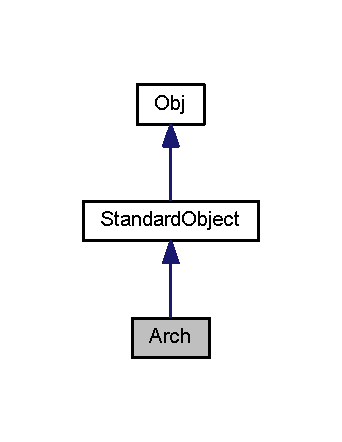
\includegraphics[width=164pt]{class_arch__inherit__graph}
\end{center}
\end{figure}


Collaboration diagram for Arch\+:
\nopagebreak
\begin{figure}[H]
\begin{center}
\leavevmode
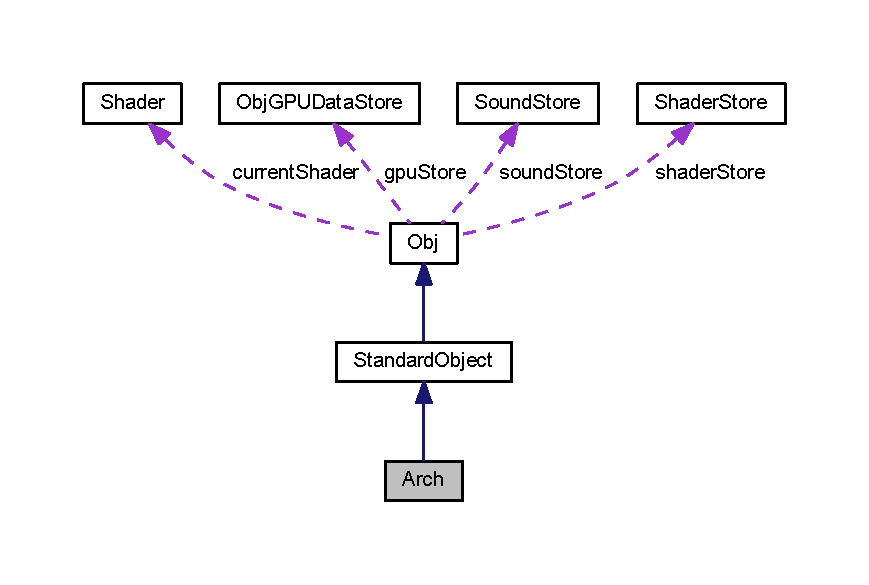
\includegraphics[width=350pt]{class_arch__coll__graph}
\end{center}
\end{figure}
\subsection*{Public Member Functions}
\begin{DoxyCompactItemize}
\item 
\hyperlink{class_arch_a147c0a492bdbe808d6853b64428fce85}{Arch} (float x, float y, bool face\+Right=false)
\begin{DoxyCompactList}\small\item\em \hyperlink{class_arch}{Arch} constructor. \end{DoxyCompactList}\end{DoxyCompactItemize}
\subsection*{Additional Inherited Members}


\subsection{Detailed Description}
The \hyperlink{class_arch}{Arch} class implements the arch used to signify the stage goal. 

\subsection{Constructor \& Destructor Documentation}
\index{Arch@{Arch}!Arch@{Arch}}
\index{Arch@{Arch}!Arch@{Arch}}
\subsubsection[{\texorpdfstring{Arch(float x, float y, bool face\+Right=false)}{Arch(float x, float y, bool faceRight=false)}}]{\setlength{\rightskip}{0pt plus 5cm}Arch\+::\+Arch (
\begin{DoxyParamCaption}
\item[{float}]{x, }
\item[{float}]{y, }
\item[{bool}]{face\+Right = {\ttfamily false}}
\end{DoxyParamCaption}
)}\hypertarget{class_arch_a147c0a492bdbe808d6853b64428fce85}{}\label{class_arch_a147c0a492bdbe808d6853b64428fce85}


\hyperlink{class_arch}{Arch} constructor. 


\begin{DoxyParams}{Parameters}
{\em x} & The x coordinate of the arch. \\
\hline
{\em y} & The y coordinate of the arch. \\
\hline
{\em face\+Right} & True if arch should face to the right (default false, i.\+e. facing left). \\
\hline
\end{DoxyParams}


The documentation for this class was generated from the following file\+:\begin{DoxyCompactItemize}
\item 
Arch.\+h\end{DoxyCompactItemize}

\hypertarget{class_boulder}{}\section{Boulder Class Reference}
\label{class_boulder}\index{Boulder@{Boulder}}


{\ttfamily \#include $<$Boulder.\+h$>$}



Inheritance diagram for Boulder\+:
\nopagebreak
\begin{figure}[H]
\begin{center}
\leavevmode
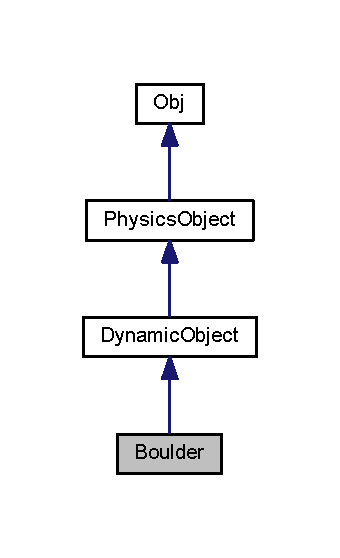
\includegraphics[width=163pt]{class_boulder__inherit__graph}
\end{center}
\end{figure}


Collaboration diagram for Boulder\+:
\nopagebreak
\begin{figure}[H]
\begin{center}
\leavevmode
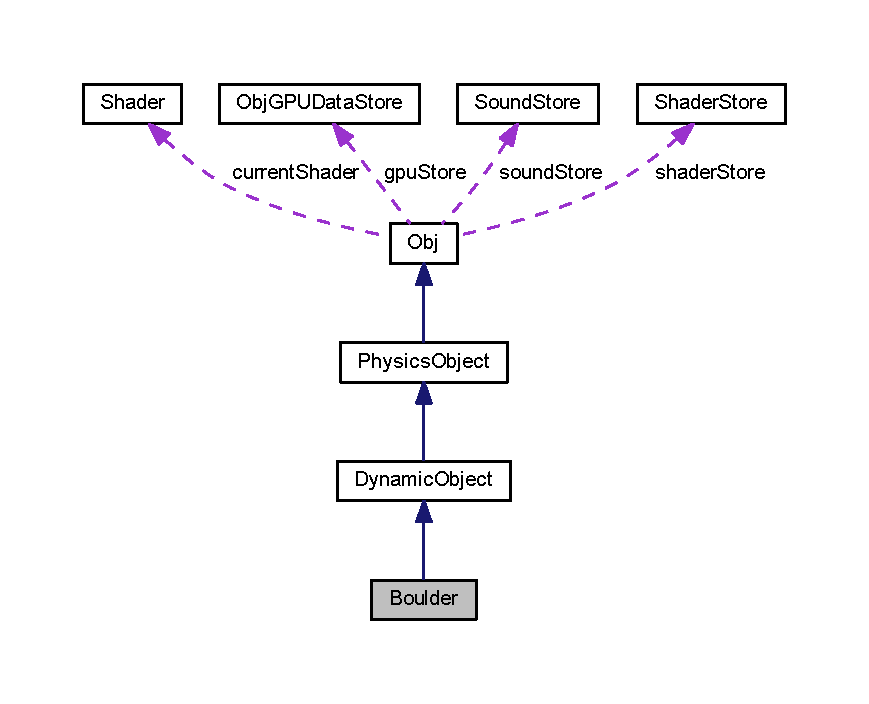
\includegraphics[width=350pt]{class_boulder__coll__graph}
\end{center}
\end{figure}
\subsection*{Public Member Functions}
\begin{DoxyCompactItemize}
\item 
\hyperlink{class_boulder_af71515f8c3676fc7bdfac71597b24b90}{Boulder} (float x, float y)
\begin{DoxyCompactList}\small\item\em \hyperlink{class_boulder}{Boulder} constructor. \end{DoxyCompactList}\end{DoxyCompactItemize}
\subsection*{Additional Inherited Members}


\subsection{Detailed Description}
The \hyperlink{class_boulder}{Boulder} class implements the boulder hazard. 

\subsection{Constructor \& Destructor Documentation}
\index{Boulder@{Boulder}!Boulder@{Boulder}}
\index{Boulder@{Boulder}!Boulder@{Boulder}}
\subsubsection[{\texorpdfstring{Boulder(float x, float y)}{Boulder(float x, float y)}}]{\setlength{\rightskip}{0pt plus 5cm}Boulder\+::\+Boulder (
\begin{DoxyParamCaption}
\item[{float}]{x, }
\item[{float}]{y}
\end{DoxyParamCaption}
)}\hypertarget{class_boulder_af71515f8c3676fc7bdfac71597b24b90}{}\label{class_boulder_af71515f8c3676fc7bdfac71597b24b90}


\hyperlink{class_boulder}{Boulder} constructor. 


\begin{DoxyParams}{Parameters}
{\em x} & The x coordinate of the boulder. \\
\hline
{\em y} & The y coordinate of the boulder. \\
\hline
\end{DoxyParams}


The documentation for this class was generated from the following file\+:\begin{DoxyCompactItemize}
\item 
Boulder.\+h\end{DoxyCompactItemize}

\hypertarget{class_boundary}{}\section{Boundary Class Reference}
\label{class_boundary}\index{Boundary@{Boundary}}


{\ttfamily \#include $<$Boundary.\+h$>$}



Inheritance diagram for Boundary\+:
\nopagebreak
\begin{figure}[H]
\begin{center}
\leavevmode
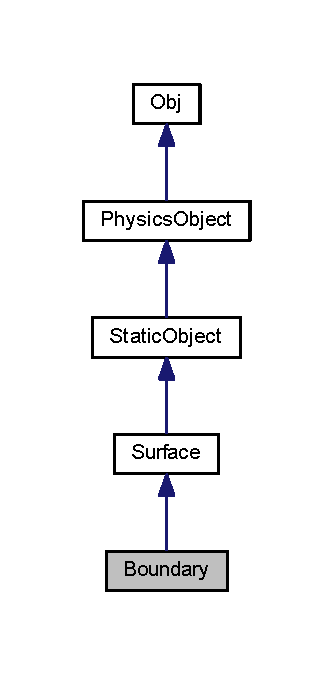
\includegraphics[width=160pt]{class_boundary__inherit__graph}
\end{center}
\end{figure}


Collaboration diagram for Boundary\+:
\nopagebreak
\begin{figure}[H]
\begin{center}
\leavevmode
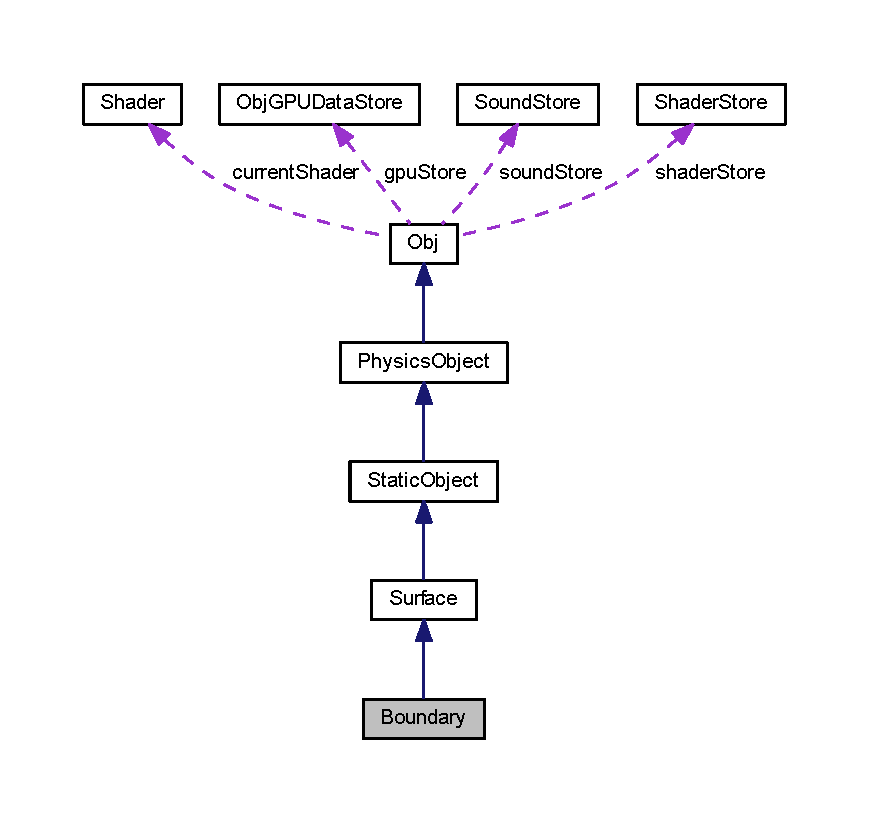
\includegraphics[width=350pt]{class_boundary__coll__graph}
\end{center}
\end{figure}
\subsection*{Public Member Functions}
\begin{DoxyCompactItemize}
\item 
\hyperlink{class_boundary_a30000217045cdef50f7c4e49b0c34fa1}{Boundary} (float x1, float x2, float y, B\+Surface surface\+Type)
\begin{DoxyCompactList}\small\item\em \hyperlink{class_boulder}{Boulder} constructor. \end{DoxyCompactList}\end{DoxyCompactItemize}
\subsection*{Additional Inherited Members}


\subsection{Detailed Description}
The \hyperlink{class_boundary}{Boundary} class implements the boundary that is used to create a surface which extends into the distance (i.\+e. creates the scene). 

\subsection{Constructor \& Destructor Documentation}
\index{Boundary@{Boundary}!Boundary@{Boundary}}
\index{Boundary@{Boundary}!Boundary@{Boundary}}
\subsubsection[{\texorpdfstring{Boundary(float x1, float x2, float y, B\+Surface surface\+Type)}{Boundary(float x1, float x2, float y, BSurface surfaceType)}}]{\setlength{\rightskip}{0pt plus 5cm}Boundary\+::\+Boundary (
\begin{DoxyParamCaption}
\item[{float}]{x1, }
\item[{float}]{x2, }
\item[{float}]{y, }
\item[{B\+Surface}]{surface\+Type}
\end{DoxyParamCaption}
)}\hypertarget{class_boundary_a30000217045cdef50f7c4e49b0c34fa1}{}\label{class_boundary_a30000217045cdef50f7c4e49b0c34fa1}


\hyperlink{class_boulder}{Boulder} constructor. 


\begin{DoxyParams}{Parameters}
{\em x1} & The leftmost extent of the boundary. \\
\hline
{\em x2} & The rightmost extent of the boundary. \\
\hline
{\em y} & The y-\/coordinate of the boundary. \\
\hline
{\em surface\+Type} & The type of surface. \\
\hline
\end{DoxyParams}


The documentation for this class was generated from the following file\+:\begin{DoxyCompactItemize}
\item 
Boundary.\+h\end{DoxyCompactItemize}

\hypertarget{class_camera}{}\section{Camera Class Reference}
\label{class_camera}\index{Camera@{Camera}}


{\ttfamily \#include $<$Camera.\+h$>$}

\subsection*{Public Member Functions}
\begin{DoxyCompactItemize}
\item 
\hyperlink{class_camera_a01f94c3543f56ede7af49dc778f19331}{Camera} ()\hypertarget{class_camera_a01f94c3543f56ede7af49dc778f19331}{}\label{class_camera_a01f94c3543f56ede7af49dc778f19331}

\begin{DoxyCompactList}\small\item\em \hyperlink{class_camera}{Camera} constructor. \end{DoxyCompactList}\item 
void \hyperlink{class_camera_a62d35e87b3eeac9463f43c17b65ef090}{zoom\+In} ()\hypertarget{class_camera_a62d35e87b3eeac9463f43c17b65ef090}{}\label{class_camera_a62d35e87b3eeac9463f43c17b65ef090}

\begin{DoxyCompactList}\small\item\em Zoom the view in. \end{DoxyCompactList}\item 
void \hyperlink{class_camera_aafc1d985053e11bd553b8a12540a562d}{zoom\+Out} ()\hypertarget{class_camera_aafc1d985053e11bd553b8a12540a562d}{}\label{class_camera_aafc1d985053e11bd553b8a12540a562d}

\begin{DoxyCompactList}\small\item\em Zoom the view out. \end{DoxyCompactList}\end{DoxyCompactItemize}
\subsection*{Public Attributes}
\begin{DoxyCompactItemize}
\item 
glm\+::vec3 \hyperlink{class_camera_a3fe5f351380fb118ffc600591769f049}{up}\hypertarget{class_camera_a3fe5f351380fb118ffc600591769f049}{}\label{class_camera_a3fe5f351380fb118ffc600591769f049}

\begin{DoxyCompactList}\small\item\em The up vector. \end{DoxyCompactList}\item 
float \hyperlink{class_camera_a21fc9e142b104d8e94126657abaa075f}{zoom}\hypertarget{class_camera_a21fc9e142b104d8e94126657abaa075f}{}\label{class_camera_a21fc9e142b104d8e94126657abaa075f}

\begin{DoxyCompactList}\small\item\em Current zoom level. \end{DoxyCompactList}\end{DoxyCompactItemize}


\subsection{Detailed Description}
The \hyperlink{class_camera}{Camera} class controls the view of the stage. 

The documentation for this class was generated from the following file\+:\begin{DoxyCompactItemize}
\item 
Camera.\+h\end{DoxyCompactItemize}

\hypertarget{class_dynamic_object}{}\section{Dynamic\+Object Class Reference}
\label{class_dynamic_object}\index{Dynamic\+Object@{Dynamic\+Object}}


{\ttfamily \#include $<$Obj.\+h$>$}

Inheritance diagram for Dynamic\+Object\+:\begin{figure}[H]
\begin{center}
\leavevmode
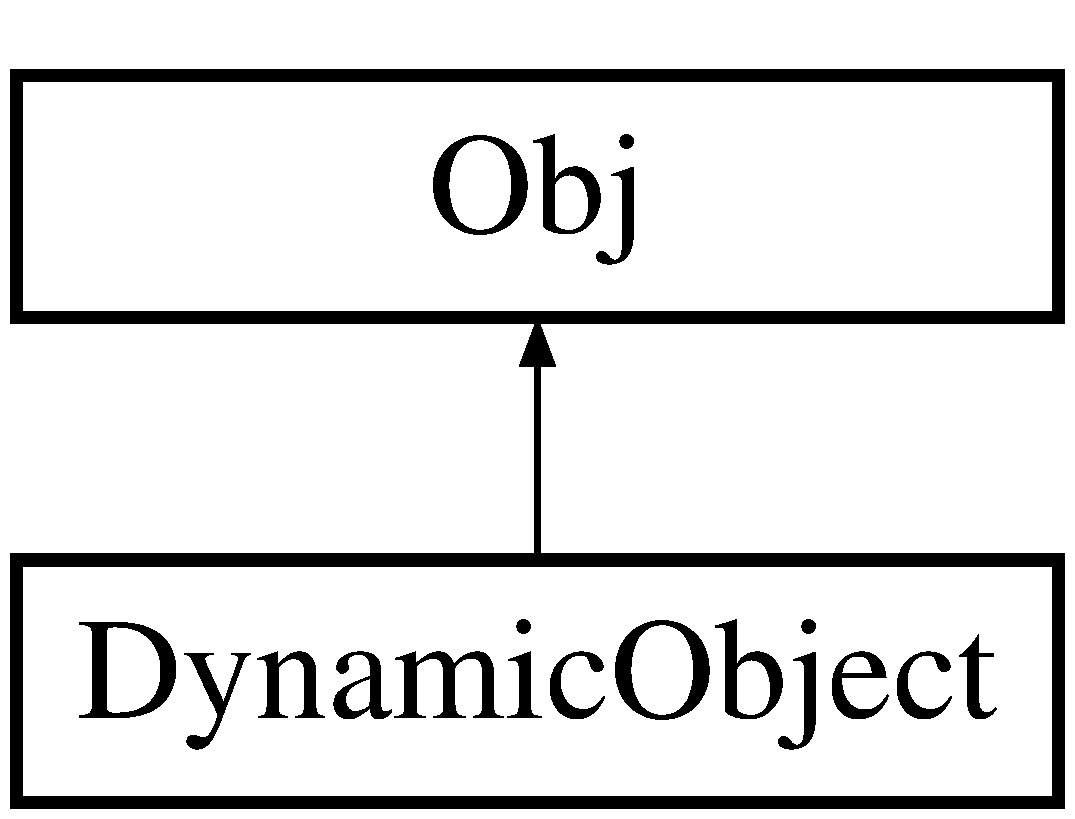
\includegraphics[height=2.000000cm]{class_dynamic_object}
\end{center}
\end{figure}
\subsection*{Public Member Functions}
\begin{DoxyCompactItemize}
\item 
\hyperlink{class_dynamic_object_a50a7adf3d7d1f411ed2aa9a663bfe275}{Dynamic\+Object} ()\hypertarget{class_dynamic_object_a50a7adf3d7d1f411ed2aa9a663bfe275}{}\label{class_dynamic_object_a50a7adf3d7d1f411ed2aa9a663bfe275}

\begin{DoxyCompactList}\small\item\em \hyperlink{class_dynamic_object}{Dynamic\+Object} constructor. \end{DoxyCompactList}\item 
\hyperlink{class_dynamic_object_a09f1992e754cb6f076923abefcb10a01}{Dynamic\+Object} (cp\+Space $\ast$space, glm\+::vec2 pos, float mass, float scale, float elast, float fric, \hyperlink{class_obj_g_p_u_data}{Obj\+G\+P\+U\+Data} $\ast$\hyperlink{class_obj_a33a9a5371319a410f7d2d395a7ef2423}{gpu\+Data}, int type, bool no\+Rotation=false)
\begin{DoxyCompactList}\small\item\em \hyperlink{class_dynamic_object}{Dynamic\+Object} constructor. \end{DoxyCompactList}\end{DoxyCompactItemize}
\subsection*{Additional Inherited Members}


\subsection{Detailed Description}
The \hyperlink{class_dynamic_object}{Dynamic\+Object} class is derived from the \hyperlink{class_obj}{Obj} class. This type of object is subject to all physics calculations. 

\subsection{Constructor \& Destructor Documentation}
\index{Dynamic\+Object@{Dynamic\+Object}!Dynamic\+Object@{Dynamic\+Object}}
\index{Dynamic\+Object@{Dynamic\+Object}!Dynamic\+Object@{Dynamic\+Object}}
\subsubsection[{\texorpdfstring{Dynamic\+Object(cp\+Space $\ast$space, glm\+::vec2 pos, float mass, float scale, float elast, float fric, Obj\+G\+P\+U\+Data $\ast$gpu\+Data, int type, bool no\+Rotation=false)}{DynamicObject(cpSpace *space, glm::vec2 pos, float mass, float scale, float elast, float fric, ObjGPUData *gpuData, int type, bool noRotation=false)}}]{\setlength{\rightskip}{0pt plus 5cm}Dynamic\+Object\+::\+Dynamic\+Object (
\begin{DoxyParamCaption}
\item[{cp\+Space $\ast$}]{space, }
\item[{glm\+::vec2}]{pos, }
\item[{float}]{mass, }
\item[{float}]{scale, }
\item[{float}]{elast, }
\item[{float}]{fric, }
\item[{{\bf Obj\+G\+P\+U\+Data} $\ast$}]{gpu\+Data, }
\item[{int}]{type, }
\item[{bool}]{no\+Rotation = {\ttfamily false}}
\end{DoxyParamCaption}
)}\hypertarget{class_dynamic_object_a09f1992e754cb6f076923abefcb10a01}{}\label{class_dynamic_object_a09f1992e754cb6f076923abefcb10a01}


\hyperlink{class_dynamic_object}{Dynamic\+Object} constructor. 


\begin{DoxyParams}{Parameters}
{\em space} & Chipmunk 2D space to attach object to \\
\hline
{\em pos} & Coordinates of the initial center of the object \\
\hline
{\em mass} & Mass of the object \\
\hline
{\em scale} & Scalar factor by which to scale the object during G\+PU rendering \\
\hline
{\em elast} & Elasticity of the object \\
\hline
{\em fric} & Friction factor of the object \\
\hline
{\em gpu\+Data} & Pointer to the gpu data associated with the object \\
\hline
{\em type} & Type of object (different values affect collision routines) \\
\hline
{\em no\+Rotation} & Flag to ignore angular momentum in the physics calculations (default = false) \\
\hline
\end{DoxyParams}

\hypertarget{class_environment}{}\section{Environment Class Reference}
\label{class_environment}\index{Environment@{Environment}}


{\ttfamily \#include $<$Environment.\+h$>$}

Inheritance diagram for Environment\+:\begin{figure}[H]
\begin{center}
\leavevmode
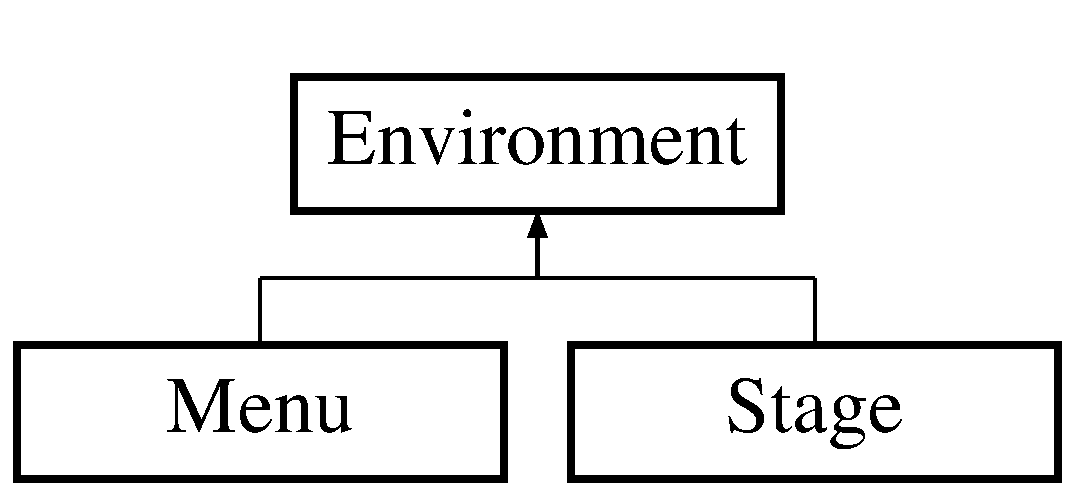
\includegraphics[height=2.000000cm]{class_environment}
\end{center}
\end{figure}
\subsection*{Public Member Functions}
\begin{DoxyCompactItemize}
\item 
virtual void \hyperlink{class_environment_afbc95329581e994ed49a678c814657ea}{update\+Environment} (double dt)=0
\begin{DoxyCompactList}\small\item\em Pure virtual function (i.\+e. defined by derived classes) for updating the environment. \end{DoxyCompactList}\item 
virtual void \hyperlink{class_environment_abcb85d008742da90125199da254c2c02}{draw\+Environment} ()=0\hypertarget{class_environment_abcb85d008742da90125199da254c2c02}{}\label{class_environment_abcb85d008742da90125199da254c2c02}

\begin{DoxyCompactList}\small\item\em Pure virtual function (i.\+e. defined by derived classes) for drawing the environment. \end{DoxyCompactList}\item 
void \hyperlink{class_environment_ac3b35b4c49e51075063e4dbed67845fb}{change\+Shader} (\hyperlink{class_shader}{Shader} $\ast$next\+Shader)
\begin{DoxyCompactList}\small\item\em Changes the shader program. \end{DoxyCompactList}\item 
virtual void \hyperlink{class_environment_a3a105533fb7592615f6b4321aafc5545}{process\+KB} (int key, int scancode, int action, int mods)=0
\begin{DoxyCompactList}\small\item\em Pure virtual function (i.\+e. defined by derived classes) for keyboard input processing. \end{DoxyCompactList}\item 
virtual void \hyperlink{class_environment_ac8157c702f012ecbdf42fc868d5164a8}{process\+Continuous\+Input} ()=0\hypertarget{class_environment_ac8157c702f012ecbdf42fc868d5164a8}{}\label{class_environment_ac8157c702f012ecbdf42fc868d5164a8}

\begin{DoxyCompactList}\small\item\em Pure virtual function (i.\+e. defined by derived classes) for continuous input processing. \end{DoxyCompactList}\item 
virtual void \hyperlink{class_environment_a6a5f1ed78138fb882a06081992c8b34a}{process\+Mouse\+Position} (float xpos, float ypos)=0
\begin{DoxyCompactList}\small\item\em Pure virtual function (i.\+e. defined by derived classes) for mouse position change processing. \end{DoxyCompactList}\item 
virtual void \hyperlink{class_environment_ae4d9f0521de194cbfd8894d97bd4cfa9}{process\+Mouse\+Click} (int button, int action, int mods, float winX, float winY)=0
\begin{DoxyCompactList}\small\item\em Pure virtual function (i.\+e. defined by derived classes) for mouse input processing. \end{DoxyCompactList}\item 
void \hyperlink{class_environment_a46e963ec1448396e116809558774ea83}{update\+Projection} (glm\+::mat4 new\+Projection)
\begin{DoxyCompactList}\small\item\em Updates the projection matrix. \end{DoxyCompactList}\end{DoxyCompactItemize}
\subsection*{Public Attributes}
\begin{DoxyCompactItemize}
\item 
int \hyperlink{class_environment_adb416d41b33612a7aeb2cd6a7aa46952}{key\+States} \mbox{[}G\+L\+F\+W\+\_\+\+K\+E\+Y\+\_\+\+L\+A\+ST\mbox{]} = \{0\}\hypertarget{class_environment_adb416d41b33612a7aeb2cd6a7aa46952}{}\label{class_environment_adb416d41b33612a7aeb2cd6a7aa46952}

\begin{DoxyCompactList}\small\item\em Array that keeps track of keyboard keys currently pressed down. \end{DoxyCompactList}\end{DoxyCompactItemize}
\subsection*{Protected Attributes}
\begin{DoxyCompactItemize}
\item 
std\+::map$<$ std\+::string, \hyperlink{class_obj_g_p_u_data}{Obj\+G\+P\+U\+Data} $\ast$ $>$ \hyperlink{class_environment_a63e85f9e330d8b15341d74e41445de72}{gpu\+Map}\hypertarget{class_environment_a63e85f9e330d8b15341d74e41445de72}{}\label{class_environment_a63e85f9e330d8b15341d74e41445de72}

\begin{DoxyCompactList}\small\item\em Stored object data used by the G\+PU (i.\+e. meshes/texture mappings/etc.). \end{DoxyCompactList}\item 
std\+::map$<$ std\+::string, \hyperlink{class_sound}{Sound} $\ast$ $>$ \hyperlink{class_environment_a69466b733dc5de97a737179db3622fc4}{sound\+Map}\hypertarget{class_environment_a69466b733dc5de97a737179db3622fc4}{}\label{class_environment_a69466b733dc5de97a737179db3622fc4}

\begin{DoxyCompactList}\small\item\em Stored sound data. \end{DoxyCompactList}\item 
std\+::map$<$ std\+::string, \hyperlink{class_shader}{Shader} $\ast$ $>$ \hyperlink{class_environment_a88eac0ec0201cebf3dba08a7bccfbd9d}{shader\+Map}\hypertarget{class_environment_a88eac0ec0201cebf3dba08a7bccfbd9d}{}\label{class_environment_a88eac0ec0201cebf3dba08a7bccfbd9d}

\begin{DoxyCompactList}\small\item\em Stored shaders. \end{DoxyCompactList}\item 
glm\+::mat4 \hyperlink{class_environment_ab30f0315cb97e5826fe81c2baee9ba2a}{mat\+\_\+\+Projection}\hypertarget{class_environment_ab30f0315cb97e5826fe81c2baee9ba2a}{}\label{class_environment_ab30f0315cb97e5826fe81c2baee9ba2a}

\begin{DoxyCompactList}\small\item\em Projection matrix. \end{DoxyCompactList}\item 
glm\+::mat4 \hyperlink{class_environment_a584ebdf6c3c8590b4d353735b3a9d873}{mat\+\_\+\+View}\hypertarget{class_environment_a584ebdf6c3c8590b4d353735b3a9d873}{}\label{class_environment_a584ebdf6c3c8590b4d353735b3a9d873}

\begin{DoxyCompactList}\small\item\em View matrix. \end{DoxyCompactList}\item 
\hyperlink{class_shader}{Shader} $\ast$ \hyperlink{class_environment_aa432f1d0568f9e8c235328a3dc6059ac}{current\+Shader}\hypertarget{class_environment_aa432f1d0568f9e8c235328a3dc6059ac}{}\label{class_environment_aa432f1d0568f9e8c235328a3dc6059ac}

\begin{DoxyCompactList}\small\item\em Pointer to the shader that is currently bound. \end{DoxyCompactList}\item 
float \hyperlink{class_environment_a6feeed21f89f92b386262a105bb40f63}{mouseX}\hypertarget{class_environment_a6feeed21f89f92b386262a105bb40f63}{}\label{class_environment_a6feeed21f89f92b386262a105bb40f63}

\begin{DoxyCompactList}\small\item\em Current position of the mouse x-\/coordinate. \end{DoxyCompactList}\item 
float \hyperlink{class_environment_afeb8f2ac0e33127ef04aa1ae710ef27c}{mouseY}\hypertarget{class_environment_afeb8f2ac0e33127ef04aa1ae710ef27c}{}\label{class_environment_afeb8f2ac0e33127ef04aa1ae710ef27c}

\begin{DoxyCompactList}\small\item\em Current position of the mouse y-\/coordinate. \end{DoxyCompactList}\end{DoxyCompactItemize}


\subsection{Detailed Description}
The \hyperlink{class_environment}{Environment} class is an abstract class that holds information about the current game state and provides function calls to update and draw the game to the screen. The \hyperlink{class_stage}{Stage} and \hyperlink{class_menu}{Menu} classes are derived from this class. 

\subsection{Member Function Documentation}
\index{Environment@{Environment}!change\+Shader@{change\+Shader}}
\index{change\+Shader@{change\+Shader}!Environment@{Environment}}
\subsubsection[{\texorpdfstring{change\+Shader(\+Shader $\ast$next\+Shader)}{changeShader(Shader *nextShader)}}]{\setlength{\rightskip}{0pt plus 5cm}void Environment\+::change\+Shader (
\begin{DoxyParamCaption}
\item[{{\bf Shader} $\ast$}]{next\+Shader}
\end{DoxyParamCaption}
)}\hypertarget{class_environment_ac3b35b4c49e51075063e4dbed67845fb}{}\label{class_environment_ac3b35b4c49e51075063e4dbed67845fb}


Changes the shader program. 


\begin{DoxyParams}{Parameters}
{\em next\+Shader} & New shader to be bound. \\
\hline
\end{DoxyParams}
\index{Environment@{Environment}!process\+KB@{process\+KB}}
\index{process\+KB@{process\+KB}!Environment@{Environment}}
\subsubsection[{\texorpdfstring{process\+K\+B(int key, int scancode, int action, int mods)=0}{processKB(int key, int scancode, int action, int mods)=0}}]{\setlength{\rightskip}{0pt plus 5cm}virtual void Environment\+::process\+KB (
\begin{DoxyParamCaption}
\item[{int}]{key, }
\item[{int}]{scancode, }
\item[{int}]{action, }
\item[{int}]{mods}
\end{DoxyParamCaption}
)\hspace{0.3cm}{\ttfamily [pure virtual]}}\hypertarget{class_environment_a3a105533fb7592615f6b4321aafc5545}{}\label{class_environment_a3a105533fb7592615f6b4321aafc5545}


Pure virtual function (i.\+e. defined by derived classes) for keyboard input processing. 


\begin{DoxyParams}{Parameters}
{\em key} & Key to which the action corresponds. \\
\hline
{\em scancode} & System specific key code. \\
\hline
{\em action} & The action (i.\+e. button up, down, held, etc.) \\
\hline
{\em mods} & Active modifiers (i.\+e. shift, control, etc.) \\
\hline
\end{DoxyParams}


Implemented in \hyperlink{class_menu_a936bec79e70b42707578af8f7d7bc1b2}{Menu}, and \hyperlink{class_stage_ab0ac39aba2fa162499d2599c981ca3ed}{Stage}.

\index{Environment@{Environment}!process\+Mouse\+Click@{process\+Mouse\+Click}}
\index{process\+Mouse\+Click@{process\+Mouse\+Click}!Environment@{Environment}}
\subsubsection[{\texorpdfstring{process\+Mouse\+Click(int button, int action, int mods, float win\+X, float win\+Y)=0}{processMouseClick(int button, int action, int mods, float winX, float winY)=0}}]{\setlength{\rightskip}{0pt plus 5cm}virtual void Environment\+::process\+Mouse\+Click (
\begin{DoxyParamCaption}
\item[{int}]{button, }
\item[{int}]{action, }
\item[{int}]{mods, }
\item[{float}]{winX, }
\item[{float}]{winY}
\end{DoxyParamCaption}
)\hspace{0.3cm}{\ttfamily [pure virtual]}}\hypertarget{class_environment_ae4d9f0521de194cbfd8894d97bd4cfa9}{}\label{class_environment_ae4d9f0521de194cbfd8894d97bd4cfa9}


Pure virtual function (i.\+e. defined by derived classes) for mouse input processing. 


\begin{DoxyParams}{Parameters}
{\em button} & Mouse button to which the action corresponds. \\
\hline
{\em action} & The action (i.\+e. button up, down, held, etc.) \\
\hline
{\em mods} & Active modifiers (i.\+e. shift, control, etc.) \\
\hline
{\em winX} & Mouse cursor x-\/position \\
\hline
{\em winY} & Mouse cursor y-\/position \\
\hline
\end{DoxyParams}


Implemented in \hyperlink{class_menu_af88e7e50de87e47c3ec841ddc6fa455a}{Menu}, and \hyperlink{class_stage_a2c54bf08d29f9f117541bf4006f58c10}{Stage}.

\index{Environment@{Environment}!process\+Mouse\+Position@{process\+Mouse\+Position}}
\index{process\+Mouse\+Position@{process\+Mouse\+Position}!Environment@{Environment}}
\subsubsection[{\texorpdfstring{process\+Mouse\+Position(float xpos, float ypos)=0}{processMousePosition(float xpos, float ypos)=0}}]{\setlength{\rightskip}{0pt plus 5cm}virtual void Environment\+::process\+Mouse\+Position (
\begin{DoxyParamCaption}
\item[{float}]{xpos, }
\item[{float}]{ypos}
\end{DoxyParamCaption}
)\hspace{0.3cm}{\ttfamily [pure virtual]}}\hypertarget{class_environment_a6a5f1ed78138fb882a06081992c8b34a}{}\label{class_environment_a6a5f1ed78138fb882a06081992c8b34a}


Pure virtual function (i.\+e. defined by derived classes) for mouse position change processing. 


\begin{DoxyParams}{Parameters}
{\em xpos} & Mouse cursor x-\/position \\
\hline
{\em ypos} & Mouse cursor y-\/position \\
\hline
\end{DoxyParams}


Implemented in \hyperlink{class_menu_ae6c6c98bf02a32ee3f87cc3a0350e6d3}{Menu}, and \hyperlink{class_stage_ae7a66771756db91c1c0bbe6ed469b9d4}{Stage}.

\index{Environment@{Environment}!update\+Environment@{update\+Environment}}
\index{update\+Environment@{update\+Environment}!Environment@{Environment}}
\subsubsection[{\texorpdfstring{update\+Environment(double dt)=0}{updateEnvironment(double dt)=0}}]{\setlength{\rightskip}{0pt plus 5cm}virtual void Environment\+::update\+Environment (
\begin{DoxyParamCaption}
\item[{double}]{dt}
\end{DoxyParamCaption}
)\hspace{0.3cm}{\ttfamily [pure virtual]}}\hypertarget{class_environment_afbc95329581e994ed49a678c814657ea}{}\label{class_environment_afbc95329581e994ed49a678c814657ea}


Pure virtual function (i.\+e. defined by derived classes) for updating the environment. 


\begin{DoxyParams}{Parameters}
{\em dt} & Time step to be used for the update (time since last update) in milliseconds. \\
\hline
\end{DoxyParams}


Implemented in \hyperlink{class_menu_a1efe72e89e793c1c6f67d16c513499e1}{Menu}, and \hyperlink{class_stage_a3b0abe7d74c6d38cfedeab84a7506816}{Stage}.

\index{Environment@{Environment}!update\+Projection@{update\+Projection}}
\index{update\+Projection@{update\+Projection}!Environment@{Environment}}
\subsubsection[{\texorpdfstring{update\+Projection(glm\+::mat4 new\+Projection)}{updateProjection(glm::mat4 newProjection)}}]{\setlength{\rightskip}{0pt plus 5cm}void Environment\+::update\+Projection (
\begin{DoxyParamCaption}
\item[{glm\+::mat4}]{new\+Projection}
\end{DoxyParamCaption}
)}\hypertarget{class_environment_a46e963ec1448396e116809558774ea83}{}\label{class_environment_a46e963ec1448396e116809558774ea83}


Updates the projection matrix. 


\begin{DoxyParams}{Parameters}
{\em new\+Projection} & New matrix to replace previous. \\
\hline
\end{DoxyParams}

\hypertarget{class_game}{}\section{Game Class Reference}
\label{class_game}\index{Game@{Game}}


{\ttfamily \#include $<$Game.\+h$>$}

\subsection*{Public Member Functions}
\begin{DoxyCompactItemize}
\item 
\hyperlink{class_game_ad59df6562a58a614fda24622d3715b65}{Game} ()\hypertarget{class_game_ad59df6562a58a614fda24622d3715b65}{}\label{class_game_ad59df6562a58a614fda24622d3715b65}

\begin{DoxyCompactList}\small\item\em \hyperlink{class_game}{Game} class constructor. \end{DoxyCompactList}\item 
\hyperlink{class_game_ae3d112ca6e0e55150d2fdbc704474530}{$\sim$\+Game} ()\hypertarget{class_game_ae3d112ca6e0e55150d2fdbc704474530}{}\label{class_game_ae3d112ca6e0e55150d2fdbc704474530}

\begin{DoxyCompactList}\small\item\em \hyperlink{class_game}{Game} class destructor. \end{DoxyCompactList}\item 
void \hyperlink{class_game_a1ab78f5ed0d5ea879157357cf2fb2afa}{run} ()\hypertarget{class_game_a1ab78f5ed0d5ea879157357cf2fb2afa}{}\label{class_game_a1ab78f5ed0d5ea879157357cf2fb2afa}

\begin{DoxyCompactList}\small\item\em Runs the game until the application is terminated (infinite loop) \end{DoxyCompactList}\item 
void \hyperlink{class_game_ace7bc47ba743c60418930ef28e670a7f}{framebuffer\+\_\+size\+\_\+callback} (G\+L\+F\+Wwindow $\ast$, int, int)\hypertarget{class_game_ace7bc47ba743c60418930ef28e670a7f}{}\label{class_game_ace7bc47ba743c60418930ef28e670a7f}

\begin{DoxyCompactList}\small\item\em G\+L\+FW window resize callback. \end{DoxyCompactList}\item 
void \hyperlink{class_game_a69df77af132026325999ae3700825e29}{key\+\_\+callback} (G\+L\+F\+Wwindow $\ast$, int, int, int, int)\hypertarget{class_game_a69df77af132026325999ae3700825e29}{}\label{class_game_a69df77af132026325999ae3700825e29}

\begin{DoxyCompactList}\small\item\em G\+L\+FW keyboard input callback. \end{DoxyCompactList}\item 
void \hyperlink{class_game_a43bf11792029b86e8a33f58a64c8d241}{mouse\+\_\+pos\+\_\+callback} (G\+L\+F\+Wwindow $\ast$, float, float)\hypertarget{class_game_a43bf11792029b86e8a33f58a64c8d241}{}\label{class_game_a43bf11792029b86e8a33f58a64c8d241}

\begin{DoxyCompactList}\small\item\em G\+L\+FW mouse position change callback. \end{DoxyCompactList}\item 
void \hyperlink{class_game_a6b75ba24ce7f9e7d2d9af45dae72e0dc}{mouse\+\_\+button\+\_\+callback} (G\+L\+F\+Wwindow $\ast$, int, int, int)\hypertarget{class_game_a6b75ba24ce7f9e7d2d9af45dae72e0dc}{}\label{class_game_a6b75ba24ce7f9e7d2d9af45dae72e0dc}

\begin{DoxyCompactList}\small\item\em G\+L\+FW mouse button input callback. \end{DoxyCompactList}\end{DoxyCompactItemize}
\subsection*{Private Attributes}
\begin{DoxyCompactItemize}
\item 
G\+L\+F\+Wwindow $\ast$ \hyperlink{class_game_ad9bc7cf39168a1ceaf77d6177116aa94}{window}\hypertarget{class_game_ad9bc7cf39168a1ceaf77d6177116aa94}{}\label{class_game_ad9bc7cf39168a1ceaf77d6177116aa94}

\begin{DoxyCompactList}\small\item\em Reference to the G\+L\+F\+Wwindow (the window) \end{DoxyCompactList}\item 
\hyperlink{class_environment}{Environment} $\ast$ \hyperlink{class_game_aacf863ae343868f6c6b83f0f324d50f1}{env}\hypertarget{class_game_aacf863ae343868f6c6b83f0f324d50f1}{}\label{class_game_aacf863ae343868f6c6b83f0f324d50f1}

\begin{DoxyCompactList}\small\item\em Reference to the current \hyperlink{class_environment}{Environment}. \end{DoxyCompactList}\item 
double \hyperlink{class_game_a1022a000bf009876854caffdec67f906}{time\+Last}\hypertarget{class_game_a1022a000bf009876854caffdec67f906}{}\label{class_game_a1022a000bf009876854caffdec67f906}

\begin{DoxyCompactList}\small\item\em Last time that was polled; used for framerate control. \end{DoxyCompactList}\item 
double \hyperlink{class_game_a2309eef4e2db7aab3c08f695b51f3958}{time\+Elapsed}\hypertarget{class_game_a2309eef4e2db7aab3c08f695b51f3958}{}\label{class_game_a2309eef4e2db7aab3c08f695b51f3958}

\begin{DoxyCompactList}\small\item\em Time elapsed since last polling of time; used for framerate control. \end{DoxyCompactList}\item 
float \hyperlink{class_game_a5262e462eeb61d8ee8424eceff2b3c43}{winX}\hypertarget{class_game_a5262e462eeb61d8ee8424eceff2b3c43}{}\label{class_game_a5262e462eeb61d8ee8424eceff2b3c43}

\begin{DoxyCompactList}\small\item\em Stores x-\/coordinate maximum of the window. \end{DoxyCompactList}\item 
float \hyperlink{class_game_a04e6773bb06f62871bcab40fc907335a}{winY}\hypertarget{class_game_a04e6773bb06f62871bcab40fc907335a}{}\label{class_game_a04e6773bb06f62871bcab40fc907335a}

\begin{DoxyCompactList}\small\item\em Stores y-\/coordinate maximum of the window. \end{DoxyCompactList}\end{DoxyCompactItemize}


\subsection{Detailed Description}
The \hyperlink{class_game}{Game} class is a representation of the game on the highest level. It handles all exchanges between the user and the game code. It keeps a reference to the game window as well as the current environment of the game (main menu, stage, etc) and acts as a bridge between the two. User inputs are intercepted through G\+L\+FW callbacks in this class and passed on for processing by the current game environment. This class is also responsible for \char`\"{}running\char`\"{} the game and sends requests for the game environment to be updated and drawn to the screen at regular intervals (framerate is controlled). 
\hypertarget{class_goal}{}\section{Goal Class Reference}
\label{class_goal}\index{Goal@{Goal}}


{\ttfamily \#include $<$Goal.\+h$>$}



Inheritance diagram for Goal\+:
\nopagebreak
\begin{figure}[H]
\begin{center}
\leavevmode
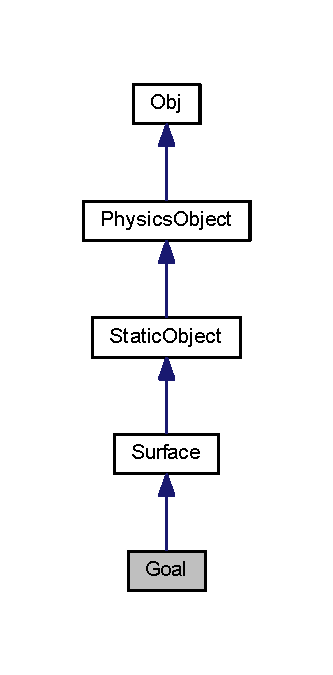
\includegraphics[width=160pt]{class_goal__inherit__graph}
\end{center}
\end{figure}


Collaboration diagram for Goal\+:
\nopagebreak
\begin{figure}[H]
\begin{center}
\leavevmode
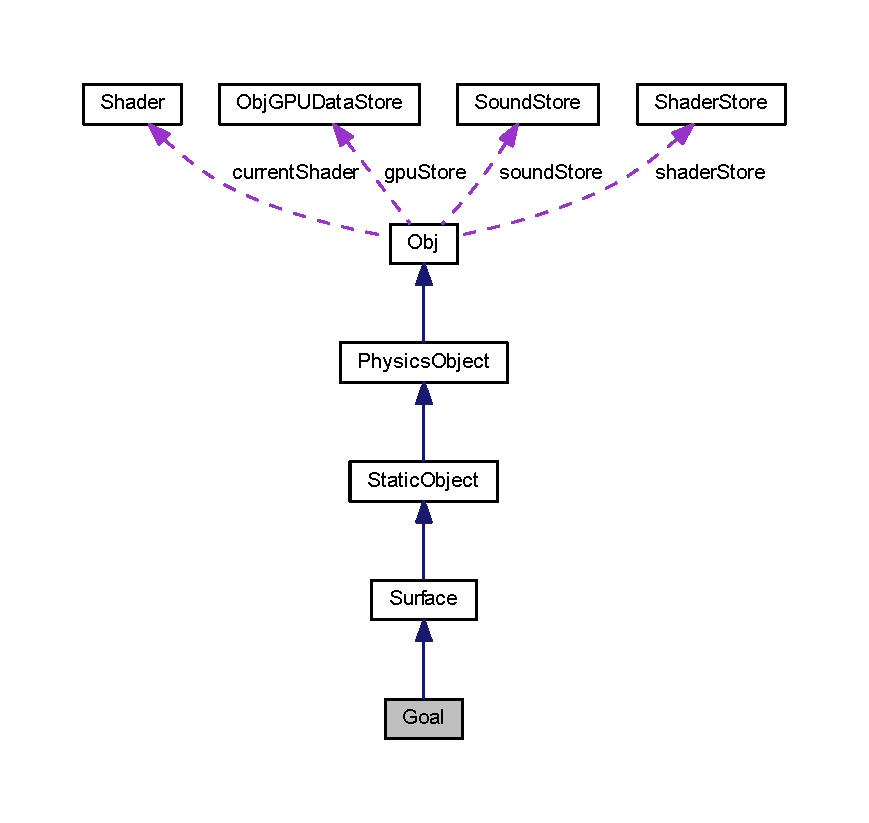
\includegraphics[width=350pt]{class_goal__coll__graph}
\end{center}
\end{figure}
\subsection*{Public Member Functions}
\begin{DoxyCompactItemize}
\item 
\hyperlink{class_goal_a5c5241cdc1ec49cb84ed86dc3749d05a}{Goal} (float x1, float x2, float ymid, float thickness=50.\+0f)
\begin{DoxyCompactList}\small\item\em \hyperlink{class_goal}{Goal} constructor. \end{DoxyCompactList}\end{DoxyCompactItemize}
\subsection*{Additional Inherited Members}


\subsection{Detailed Description}
The \hyperlink{class_goal}{Goal} class implements the checkered goal platform. 

\subsection{Constructor \& Destructor Documentation}
\index{Goal@{Goal}!Goal@{Goal}}
\index{Goal@{Goal}!Goal@{Goal}}
\subsubsection[{\texorpdfstring{Goal(float x1, float x2, float ymid, float thickness=50.\+0f)}{Goal(float x1, float x2, float ymid, float thickness=50.0f)}}]{\setlength{\rightskip}{0pt plus 5cm}Goal\+::\+Goal (
\begin{DoxyParamCaption}
\item[{float}]{x1, }
\item[{float}]{x2, }
\item[{float}]{ymid, }
\item[{float}]{thickness = {\ttfamily 50.0f}}
\end{DoxyParamCaption}
)}\hypertarget{class_goal_a5c5241cdc1ec49cb84ed86dc3749d05a}{}\label{class_goal_a5c5241cdc1ec49cb84ed86dc3749d05a}


\hyperlink{class_goal}{Goal} constructor. 


\begin{DoxyParams}{Parameters}
{\em x1} & The leftmost extent of the goal. \\
\hline
{\em x2} & The rightmost extent of the goal. \\
\hline
{\em ymid} & The y-\/coordinate of the goal. \\
\hline
{\em thickness} & The vertical thickness of the goal (default = 50.\+0). \\
\hline
\end{DoxyParams}


The documentation for this class was generated from the following file\+:\begin{DoxyCompactItemize}
\item 
Goal.\+h\end{DoxyCompactItemize}

\hypertarget{class_hero}{}\section{Hero Class Reference}
\label{class_hero}\index{Hero@{Hero}}


{\ttfamily \#include $<$Hero.\+h$>$}



Inheritance diagram for Hero\+:
\nopagebreak
\begin{figure}[H]
\begin{center}
\leavevmode
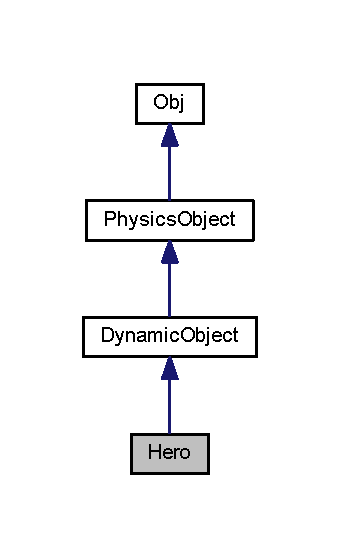
\includegraphics[width=163pt]{class_hero__inherit__graph}
\end{center}
\end{figure}


Collaboration diagram for Hero\+:
\nopagebreak
\begin{figure}[H]
\begin{center}
\leavevmode
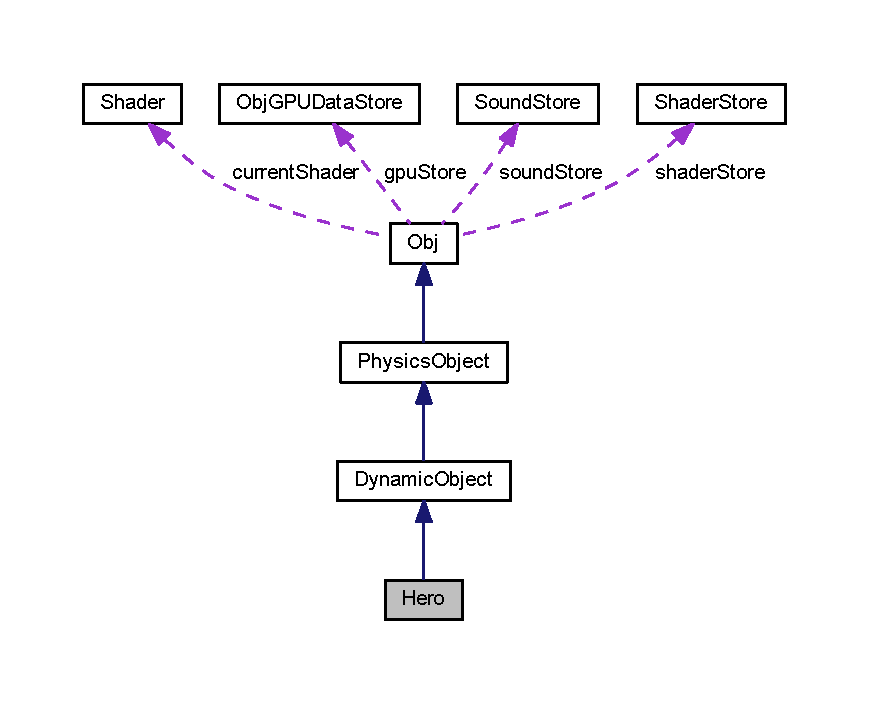
\includegraphics[width=350pt]{class_hero__coll__graph}
\end{center}
\end{figure}
\subsection*{Public Member Functions}
\begin{DoxyCompactItemize}
\item 
\hyperlink{class_hero_a8deb36af7263b83c52e62a98f31ea5cb}{Hero} (float x, float y)
\begin{DoxyCompactList}\small\item\em \hyperlink{class_hero}{Hero} constructor. \end{DoxyCompactList}\item 
void \hyperlink{class_hero_a62d93b951b0b769c75ddbdf1615660a0}{death} ()\hypertarget{class_hero_a62d93b951b0b769c75ddbdf1615660a0}{}\label{class_hero_a62d93b951b0b769c75ddbdf1615660a0}

\begin{DoxyCompactList}\small\item\em Kills the hero and resets the stage. \end{DoxyCompactList}\item 
void \hyperlink{class_hero_a1bee38d9164cf1ecda512cc24e81b171}{jump} ()\hypertarget{class_hero_a1bee38d9164cf1ecda512cc24e81b171}{}\label{class_hero_a1bee38d9164cf1ecda512cc24e81b171}

\begin{DoxyCompactList}\small\item\em Makes the hero jump. \end{DoxyCompactList}\item 
void \hyperlink{class_hero_a871ff7549c75b1099ff9b13bf6c41cf3}{win} ()\hypertarget{class_hero_a871ff7549c75b1099ff9b13bf6c41cf3}{}\label{class_hero_a871ff7549c75b1099ff9b13bf6c41cf3}

\begin{DoxyCompactList}\small\item\em Play stage win fanfare and set the level\+Win flag. \end{DoxyCompactList}\end{DoxyCompactItemize}
\subsection*{Public Attributes}
\begin{DoxyCompactItemize}
\item 
cp\+Vect \hyperlink{class_hero_a7a1e815197c299636156836ece73a4c9}{start\+Pos}\hypertarget{class_hero_a7a1e815197c299636156836ece73a4c9}{}\label{class_hero_a7a1e815197c299636156836ece73a4c9}

\begin{DoxyCompactList}\small\item\em \hyperlink{class_hero}{Hero} starting position. \end{DoxyCompactList}\item 
bool \hyperlink{class_hero_a77118f01c205e10585fa6fbd4624a056}{dead}\hypertarget{class_hero_a77118f01c205e10585fa6fbd4624a056}{}\label{class_hero_a77118f01c205e10585fa6fbd4624a056}

\begin{DoxyCompactList}\small\item\em Flag indicates if the hero is dead. \end{DoxyCompactList}\item 
bool \hyperlink{class_hero_a3ba2c1501a4a2ee6ce66ac899ee01a75}{can\+Jump}\hypertarget{class_hero_a3ba2c1501a4a2ee6ce66ac899ee01a75}{}\label{class_hero_a3ba2c1501a4a2ee6ce66ac899ee01a75}

\begin{DoxyCompactList}\small\item\em Flag indicates if the hero is currently allowed to jump. \end{DoxyCompactList}\item 
cp\+Vect \hyperlink{class_hero_aab7d3e7f06a315a9834105ea4b433f93}{rel\+Vel}\hypertarget{class_hero_aab7d3e7f06a315a9834105ea4b433f93}{}\label{class_hero_aab7d3e7f06a315a9834105ea4b433f93}

\begin{DoxyCompactList}\small\item\em Velocity relative to the surface the hero is currently on (undefined if not on surface) \end{DoxyCompactList}\item 
bool \hyperlink{class_hero_ab2a773c753e762df2bc24d582389360b}{level\+Win}\hypertarget{class_hero_ab2a773c753e762df2bc24d582389360b}{}\label{class_hero_ab2a773c753e762df2bc24d582389360b}

\begin{DoxyCompactList}\small\item\em Flag indicates if hero has reached the goal. \end{DoxyCompactList}\end{DoxyCompactItemize}
\subsection*{Additional Inherited Members}


\subsection{Detailed Description}
The \hyperlink{class_hero}{Hero} class implements the hero. 

\subsection{Constructor \& Destructor Documentation}
\index{Hero@{Hero}!Hero@{Hero}}
\index{Hero@{Hero}!Hero@{Hero}}
\subsubsection[{\texorpdfstring{Hero(float x, float y)}{Hero(float x, float y)}}]{\setlength{\rightskip}{0pt plus 5cm}Hero\+::\+Hero (
\begin{DoxyParamCaption}
\item[{float}]{x, }
\item[{float}]{y}
\end{DoxyParamCaption}
)}\hypertarget{class_hero_a8deb36af7263b83c52e62a98f31ea5cb}{}\label{class_hero_a8deb36af7263b83c52e62a98f31ea5cb}


\hyperlink{class_hero}{Hero} constructor. 


\begin{DoxyParams}{Parameters}
{\em x} & The x coordinate of the hero. \\
\hline
{\em y} & The y coordinate of the hero. \\
\hline
\end{DoxyParams}


The documentation for this class was generated from the following file\+:\begin{DoxyCompactItemize}
\item 
Hero.\+h\end{DoxyCompactItemize}

\hypertarget{class_kinematic_object}{}\section{Kinematic\+Object Class Reference}
\label{class_kinematic_object}\index{Kinematic\+Object@{Kinematic\+Object}}


{\ttfamily \#include $<$Obj.\+h$>$}

Inheritance diagram for Kinematic\+Object\+:\begin{figure}[H]
\begin{center}
\leavevmode
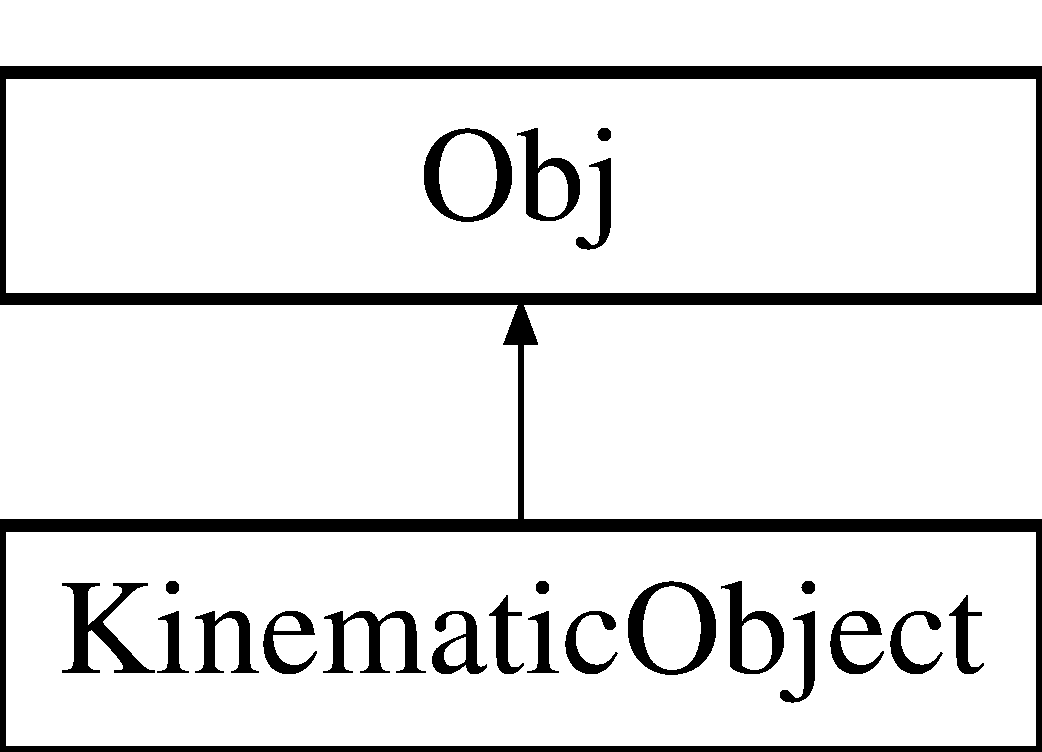
\includegraphics[height=2.000000cm]{class_kinematic_object}
\end{center}
\end{figure}
\subsection*{Public Member Functions}
\begin{DoxyCompactItemize}
\item 
\hyperlink{class_kinematic_object_a1ca8df2b3de129f3c820629b9a7ce039}{Kinematic\+Object} (cp\+Space $\ast$space, cp\+Vect p1, cp\+Vect p2, \hyperlink{class_obj_g_p_u_data}{Obj\+G\+P\+U\+Data} $\ast$\hyperlink{class_obj_a33a9a5371319a410f7d2d395a7ef2423}{gpu\+Data}, int type)
\begin{DoxyCompactList}\small\item\em \hyperlink{class_dynamic_object}{Dynamic\+Object} constructor. \end{DoxyCompactList}\end{DoxyCompactItemize}
\subsection*{Additional Inherited Members}


\subsection{Detailed Description}
The \hyperlink{class_kinematic_object}{Kinematic\+Object} class is derived from the \hyperlink{class_obj}{Obj} class. This type of object has features of both static objects and dynamic objects and is generally used for moving platforms. 

\subsection{Constructor \& Destructor Documentation}
\index{Kinematic\+Object@{Kinematic\+Object}!Kinematic\+Object@{Kinematic\+Object}}
\index{Kinematic\+Object@{Kinematic\+Object}!Kinematic\+Object@{Kinematic\+Object}}
\subsubsection[{\texorpdfstring{Kinematic\+Object(cp\+Space $\ast$space, cp\+Vect p1, cp\+Vect p2, Obj\+G\+P\+U\+Data $\ast$gpu\+Data, int type)}{KinematicObject(cpSpace *space, cpVect p1, cpVect p2, ObjGPUData *gpuData, int type)}}]{\setlength{\rightskip}{0pt plus 5cm}Kinematic\+Object\+::\+Kinematic\+Object (
\begin{DoxyParamCaption}
\item[{cp\+Space $\ast$}]{space, }
\item[{cp\+Vect}]{p1, }
\item[{cp\+Vect}]{p2, }
\item[{{\bf Obj\+G\+P\+U\+Data} $\ast$}]{gpu\+Data, }
\item[{int}]{type}
\end{DoxyParamCaption}
)}\hypertarget{class_kinematic_object_a1ca8df2b3de129f3c820629b9a7ce039}{}\label{class_kinematic_object_a1ca8df2b3de129f3c820629b9a7ce039}


\hyperlink{class_dynamic_object}{Dynamic\+Object} constructor. 


\begin{DoxyParams}{Parameters}
{\em space} & Chipmunk 2D space to attach object to \\
\hline
{\em p1} & Bottom left coordinate of bounding box \\
\hline
{\em p2} & Upper right coordinate of bounding box \\
\hline
{\em gpu\+Data} & Pointer to the gpu data associated with the object \\
\hline
{\em type} & Type of object (different values affect collision routines) \\
\hline
\end{DoxyParams}

\hypertarget{class_menu}{}\section{Menu Class Reference}
\label{class_menu}\index{Menu@{Menu}}


{\ttfamily \#include $<$Menu.\+h$>$}



Inheritance diagram for Menu\+:
\nopagebreak
\begin{figure}[H]
\begin{center}
\leavevmode
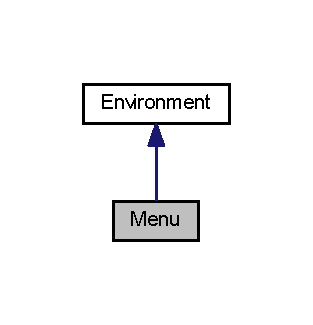
\includegraphics[width=150pt]{class_menu__inherit__graph}
\end{center}
\end{figure}


Collaboration diagram for Menu\+:
\nopagebreak
\begin{figure}[H]
\begin{center}
\leavevmode
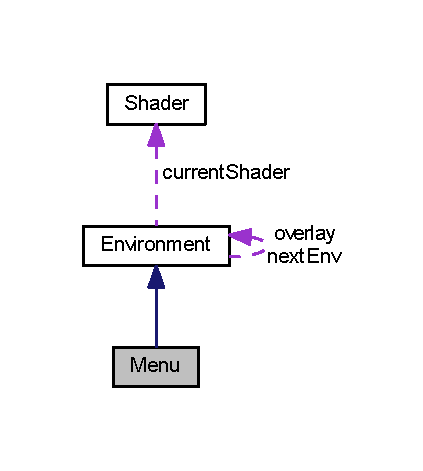
\includegraphics[width=203pt]{class_menu__coll__graph}
\end{center}
\end{figure}
\subsection*{Public Member Functions}
\begin{DoxyCompactItemize}
\item 
\hyperlink{class_menu_a7570644ca93aaf710f7ded2e20e36186}{Menu} (bool in\+Game)\hypertarget{class_menu_a7570644ca93aaf710f7ded2e20e36186}{}\label{class_menu_a7570644ca93aaf710f7ded2e20e36186}

\begin{DoxyCompactList}\small\item\em \hyperlink{class_menu}{Menu} constructor. \end{DoxyCompactList}\item 
\hyperlink{class_menu_a831387f51358cfb88cd018e1777bc980}{$\sim$\+Menu} ()\hypertarget{class_menu_a831387f51358cfb88cd018e1777bc980}{}\label{class_menu_a831387f51358cfb88cd018e1777bc980}

\begin{DoxyCompactList}\small\item\em \hyperlink{class_menu}{Menu} destructor. \end{DoxyCompactList}\item 
void \hyperlink{class_menu_a1efe72e89e793c1c6f67d16c513499e1}{update\+Environment} (double dt)
\begin{DoxyCompactList}\small\item\em Function for updating the environment. \end{DoxyCompactList}\item 
void \hyperlink{class_menu_ac1403e071d911bf4c3b43d344d46ee4f}{draw\+Environment} ()\hypertarget{class_menu_ac1403e071d911bf4c3b43d344d46ee4f}{}\label{class_menu_ac1403e071d911bf4c3b43d344d46ee4f}

\begin{DoxyCompactList}\small\item\em Function for drawing the environment. \end{DoxyCompactList}\item 
void \hyperlink{class_menu_a936bec79e70b42707578af8f7d7bc1b2}{process\+KB} (int key, int scancode, int action, int mods)
\begin{DoxyCompactList}\small\item\em Function for keyboard input processing. \end{DoxyCompactList}\item 
void \hyperlink{class_menu_a2ff354c6e9693f559f3778d78a34e405}{process\+Continuous\+Input} ()\hypertarget{class_menu_a2ff354c6e9693f559f3778d78a34e405}{}\label{class_menu_a2ff354c6e9693f559f3778d78a34e405}

\begin{DoxyCompactList}\small\item\em Function for continuous input processing. \end{DoxyCompactList}\item 
bool \hyperlink{class_menu_a98aa69e5ed8eb5a80cd19b4dd6c9482c}{process\+Mouse\+Position} (float xpos, float ypos)
\begin{DoxyCompactList}\small\item\em Function for mouse position change processing. \end{DoxyCompactList}\item 
void \hyperlink{class_menu_acf97e448b5fbe3fefca5e6459e841438}{process\+Mouse\+Click} (int button, int action, int mods)
\begin{DoxyCompactList}\small\item\em Function for mouse input processing. \end{DoxyCompactList}\item 
void \hyperlink{class_menu_adc7835954b600003eea158e03a0108d4}{Show\+Sub\+Menu} (int level, bool b\+Show=true)
\begin{DoxyCompactList}\small\item\em Displays main menu. \end{DoxyCompactList}\item 
void \hyperlink{class_menu_a0f4426bd7323a84c24fc764a76f0b557}{show\+Level\+Sub\+Menu} (bool b\+Show)
\begin{DoxyCompactList}\small\item\em Displays level select menu. \end{DoxyCompactList}\item 
void \hyperlink{class_menu_a6599ad763c91acb0a1683be542f8e095}{update\+Screen\+Size} ()\hypertarget{class_menu_a6599ad763c91acb0a1683be542f8e095}{}\label{class_menu_a6599ad763c91acb0a1683be542f8e095}

\begin{DoxyCompactList}\small\item\em Changes layout due to screen size update. \end{DoxyCompactList}\item 
void \hyperlink{class_menu_a085252eb220290c5492a3afca26fa2a1}{add\+New\+Item} (char $\ast$sz\+Normal, char $\ast$sz\+Hover, char $\ast$sz\+Selected, int posX, int posY, Menu\+Item\+Handler handler, void $\ast$param, short level, bool active=false, bool fixed=false)\hypertarget{class_menu_a085252eb220290c5492a3afca26fa2a1}{}\label{class_menu_a085252eb220290c5492a3afca26fa2a1}

\begin{DoxyCompactList}\small\item\em Adds button to the menu. \end{DoxyCompactList}\end{DoxyCompactItemize}
\subsection*{Private Member Functions}
\begin{DoxyCompactItemize}
\item 
void \hyperlink{class_menu_a7e39cf7f3f6404eb670e34f4e4303f92}{hover\+\_\+menuitem} (Menu\+Item $\ast$)\hypertarget{class_menu_a7e39cf7f3f6404eb670e34f4e4303f92}{}\label{class_menu_a7e39cf7f3f6404eb670e34f4e4303f92}

\begin{DoxyCompactList}\small\item\em Called when mouse position is changes to detect hover over buttons. \end{DoxyCompactList}\item 
void \hyperlink{class_menu_a1bc5693b23c0545f153b8d472256b672}{click\+\_\+menuitem} (Menu\+Item $\ast$)\hypertarget{class_menu_a1bc5693b23c0545f153b8d472256b672}{}\label{class_menu_a1bc5693b23c0545f153b8d472256b672}

\begin{DoxyCompactList}\small\item\em Called when mouse is clicked to detect click on buttons. \end{DoxyCompactList}\end{DoxyCompactItemize}
\subsection*{Private Attributes}
\begin{DoxyCompactItemize}
\item 
std\+::vector$<$ Menu\+Item $\ast$ $>$ \hyperlink{class_menu_a5392cc6eccd7473ee634e976106466d9}{vec\+Menu\+Item}\hypertarget{class_menu_a5392cc6eccd7473ee634e976106466d9}{}\label{class_menu_a5392cc6eccd7473ee634e976106466d9}

\begin{DoxyCompactList}\small\item\em Stores menu buttons. \end{DoxyCompactList}\end{DoxyCompactItemize}
\subsection*{Additional Inherited Members}


\subsection{Detailed Description}
The \hyperlink{class_menu}{Menu} class is derived from the \hyperlink{class_environment}{Environment} class and holds and handles changes to the game state when the user is not playing a stage (i.\+e. is in a menu of some kind). 

\subsection{Member Function Documentation}
\index{Menu@{Menu}!process\+KB@{process\+KB}}
\index{process\+KB@{process\+KB}!Menu@{Menu}}
\subsubsection[{\texorpdfstring{process\+K\+B(int key, int scancode, int action, int mods)}{processKB(int key, int scancode, int action, int mods)}}]{\setlength{\rightskip}{0pt plus 5cm}void Menu\+::process\+KB (
\begin{DoxyParamCaption}
\item[{int}]{key, }
\item[{int}]{scancode, }
\item[{int}]{action, }
\item[{int}]{mods}
\end{DoxyParamCaption}
)\hspace{0.3cm}{\ttfamily [virtual]}}\hypertarget{class_menu_a936bec79e70b42707578af8f7d7bc1b2}{}\label{class_menu_a936bec79e70b42707578af8f7d7bc1b2}


Function for keyboard input processing. 


\begin{DoxyParams}{Parameters}
{\em key} & Key to which the action corresponds. \\
\hline
{\em scancode} & System specific key code. \\
\hline
{\em action} & The action (i.\+e. button up, down, held, etc.) \\
\hline
{\em mods} & Active modifiers (i.\+e. shift, control, etc.) \\
\hline
\end{DoxyParams}


Implements \hyperlink{class_environment_a3a105533fb7592615f6b4321aafc5545}{Environment}.

\index{Menu@{Menu}!process\+Mouse\+Click@{process\+Mouse\+Click}}
\index{process\+Mouse\+Click@{process\+Mouse\+Click}!Menu@{Menu}}
\subsubsection[{\texorpdfstring{process\+Mouse\+Click(int button, int action, int mods)}{processMouseClick(int button, int action, int mods)}}]{\setlength{\rightskip}{0pt plus 5cm}void Menu\+::process\+Mouse\+Click (
\begin{DoxyParamCaption}
\item[{int}]{button, }
\item[{int}]{action, }
\item[{int}]{mods}
\end{DoxyParamCaption}
)\hspace{0.3cm}{\ttfamily [virtual]}}\hypertarget{class_menu_acf97e448b5fbe3fefca5e6459e841438}{}\label{class_menu_acf97e448b5fbe3fefca5e6459e841438}


Function for mouse input processing. 


\begin{DoxyParams}{Parameters}
{\em button} & Mouse button to which the action corresponds. \\
\hline
{\em action} & The action (i.\+e. button up, down, held, etc.) \\
\hline
{\em mods} & Active modifiers (i.\+e. shift, control, etc.) \\
\hline
\end{DoxyParams}


Implements \hyperlink{class_environment_a19cf4bbbe86528759e0ad79e19025732}{Environment}.

\index{Menu@{Menu}!process\+Mouse\+Position@{process\+Mouse\+Position}}
\index{process\+Mouse\+Position@{process\+Mouse\+Position}!Menu@{Menu}}
\subsubsection[{\texorpdfstring{process\+Mouse\+Position(float xpos, float ypos)}{processMousePosition(float xpos, float ypos)}}]{\setlength{\rightskip}{0pt plus 5cm}bool Menu\+::process\+Mouse\+Position (
\begin{DoxyParamCaption}
\item[{float}]{xpos, }
\item[{float}]{ypos}
\end{DoxyParamCaption}
)\hspace{0.3cm}{\ttfamily [virtual]}}\hypertarget{class_menu_a98aa69e5ed8eb5a80cd19b4dd6c9482c}{}\label{class_menu_a98aa69e5ed8eb5a80cd19b4dd6c9482c}


Function for mouse position change processing. 


\begin{DoxyParams}{Parameters}
{\em xpos} & Mouse cursor x-\/position \\
\hline
{\em ypos} & Mouse cursor y-\/position \\
\hline
\end{DoxyParams}


Implements \hyperlink{class_environment_a92819bf5a6aa5877c0f89fd65a4d7554}{Environment}.

\index{Menu@{Menu}!show\+Level\+Sub\+Menu@{show\+Level\+Sub\+Menu}}
\index{show\+Level\+Sub\+Menu@{show\+Level\+Sub\+Menu}!Menu@{Menu}}
\subsubsection[{\texorpdfstring{show\+Level\+Sub\+Menu(bool b\+Show)}{showLevelSubMenu(bool bShow)}}]{\setlength{\rightskip}{0pt plus 5cm}void Menu\+::show\+Level\+Sub\+Menu (
\begin{DoxyParamCaption}
\item[{bool}]{b\+Show}
\end{DoxyParamCaption}
)}\hypertarget{class_menu_a0f4426bd7323a84c24fc764a76f0b557}{}\label{class_menu_a0f4426bd7323a84c24fc764a76f0b557}


Displays level select menu. 


\begin{DoxyParams}{Parameters}
{\em b\+Show} & Flag specifies whether buttons should be drawn. \\
\hline
\end{DoxyParams}
\index{Menu@{Menu}!Show\+Sub\+Menu@{Show\+Sub\+Menu}}
\index{Show\+Sub\+Menu@{Show\+Sub\+Menu}!Menu@{Menu}}
\subsubsection[{\texorpdfstring{Show\+Sub\+Menu(int level, bool b\+Show=true)}{ShowSubMenu(int level, bool bShow=true)}}]{\setlength{\rightskip}{0pt plus 5cm}void Menu\+::\+Show\+Sub\+Menu (
\begin{DoxyParamCaption}
\item[{int}]{level, }
\item[{bool}]{b\+Show = {\ttfamily true}}
\end{DoxyParamCaption}
)}\hypertarget{class_menu_adc7835954b600003eea158e03a0108d4}{}\label{class_menu_adc7835954b600003eea158e03a0108d4}


Displays main menu. 


\begin{DoxyParams}{Parameters}
{\em level} & \hyperlink{class_menu}{Menu} depth. \\
\hline
{\em b\+Show} & Flag specifies whether buttons should be drawn. \\
\hline
\end{DoxyParams}
\index{Menu@{Menu}!update\+Environment@{update\+Environment}}
\index{update\+Environment@{update\+Environment}!Menu@{Menu}}
\subsubsection[{\texorpdfstring{update\+Environment(double dt)}{updateEnvironment(double dt)}}]{\setlength{\rightskip}{0pt plus 5cm}void Menu\+::update\+Environment (
\begin{DoxyParamCaption}
\item[{double}]{dt}
\end{DoxyParamCaption}
)\hspace{0.3cm}{\ttfamily [virtual]}}\hypertarget{class_menu_a1efe72e89e793c1c6f67d16c513499e1}{}\label{class_menu_a1efe72e89e793c1c6f67d16c513499e1}


Function for updating the environment. 


\begin{DoxyParams}{Parameters}
{\em dt} & Time step to be used for the update (time since last update) in milliseconds. \\
\hline
\end{DoxyParams}


Implements \hyperlink{class_environment_afbc95329581e994ed49a678c814657ea}{Environment}.



The documentation for this class was generated from the following file\+:\begin{DoxyCompactItemize}
\item 
Menu.\+h\end{DoxyCompactItemize}

\hypertarget{class_moving_platform}{}\section{Moving\+Platform Class Reference}
\label{class_moving_platform}\index{Moving\+Platform@{Moving\+Platform}}


{\ttfamily \#include $<$Moving\+Platform.\+h$>$}



Inheritance diagram for Moving\+Platform\+:
\nopagebreak
\begin{figure}[H]
\begin{center}
\leavevmode
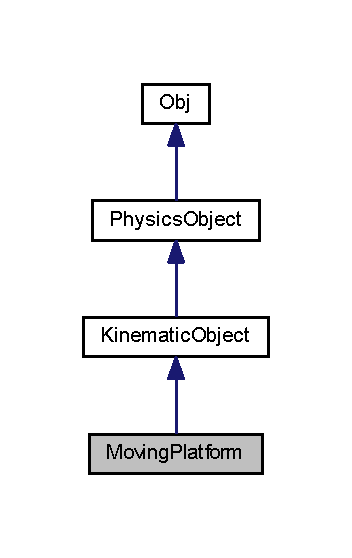
\includegraphics[width=169pt]{class_moving_platform__inherit__graph}
\end{center}
\end{figure}


Collaboration diagram for Moving\+Platform\+:
\nopagebreak
\begin{figure}[H]
\begin{center}
\leavevmode
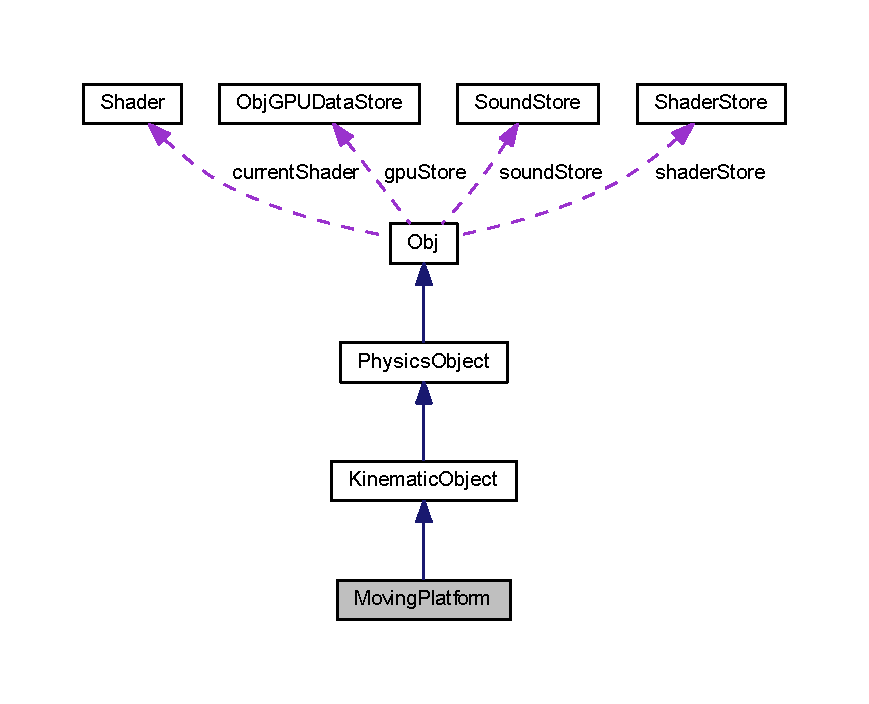
\includegraphics[width=350pt]{class_moving_platform__coll__graph}
\end{center}
\end{figure}
\subsection*{Public Member Functions}
\begin{DoxyCompactItemize}
\item 
\hyperlink{class_moving_platform_ac33dba37c6bbd2e496f157ac5f2fcf6b}{Moving\+Platform} (float w, float \hyperlink{class_moving_platform_a71db6ff1f8e4b94445e096ca62d79df4}{speed}, std\+::vector$<$ cp\+Vect $>$ \&\hyperlink{class_moving_platform_a35dc1c58256404b865365f634588ce38}{path}, float thickness=50.\+0f)
\begin{DoxyCompactList}\small\item\em Creates a new moving platform. \end{DoxyCompactList}\item 
void \hyperlink{class_moving_platform_a9eb48b9e90a70b28f6c71ec2673a66cc}{update} (float dt)
\begin{DoxyCompactList}\small\item\em Updates platform position. \end{DoxyCompactList}\end{DoxyCompactItemize}
\subsection*{Private Attributes}
\begin{DoxyCompactItemize}
\item 
int \hyperlink{class_moving_platform_a58664732e195a862557bf26f68b7a8ef}{dir}\hypertarget{class_moving_platform_a58664732e195a862557bf26f68b7a8ef}{}\label{class_moving_platform_a58664732e195a862557bf26f68b7a8ef}

\begin{DoxyCompactList}\small\item\em Direction of movement. \end{DoxyCompactList}\item 
float \hyperlink{class_moving_platform_a71db6ff1f8e4b94445e096ca62d79df4}{speed}\hypertarget{class_moving_platform_a71db6ff1f8e4b94445e096ca62d79df4}{}\label{class_moving_platform_a71db6ff1f8e4b94445e096ca62d79df4}

\begin{DoxyCompactList}\small\item\em Speed of movement. \end{DoxyCompactList}\item 
int \hyperlink{class_moving_platform_af5cbf79f35bbaf062069d66ac0d566ea}{destination\+Node}\hypertarget{class_moving_platform_af5cbf79f35bbaf062069d66ac0d566ea}{}\label{class_moving_platform_af5cbf79f35bbaf062069d66ac0d566ea}

\begin{DoxyCompactList}\small\item\em Node that the platform is headed to. \end{DoxyCompactList}\item 
std\+::vector$<$ cp\+Vect $>$ \hyperlink{class_moving_platform_a35dc1c58256404b865365f634588ce38}{path}\hypertarget{class_moving_platform_a35dc1c58256404b865365f634588ce38}{}\label{class_moving_platform_a35dc1c58256404b865365f634588ce38}

\begin{DoxyCompactList}\small\item\em The path the platform takes. \end{DoxyCompactList}\end{DoxyCompactItemize}
\subsection*{Additional Inherited Members}


\subsection{Detailed Description}
The \hyperlink{class_moving_platform}{Moving\+Platform} class implements moving platforms. 

\subsection{Constructor \& Destructor Documentation}
\index{Moving\+Platform@{Moving\+Platform}!Moving\+Platform@{Moving\+Platform}}
\index{Moving\+Platform@{Moving\+Platform}!Moving\+Platform@{Moving\+Platform}}
\subsubsection[{\texorpdfstring{Moving\+Platform(float w, float speed, std\+::vector$<$ cp\+Vect $>$ \&path, float thickness=50.\+0f)}{MovingPlatform(float w, float speed, std::vector< cpVect > &path, float thickness=50.0f)}}]{\setlength{\rightskip}{0pt plus 5cm}Moving\+Platform\+::\+Moving\+Platform (
\begin{DoxyParamCaption}
\item[{float}]{w, }
\item[{float}]{speed, }
\item[{std\+::vector$<$ cp\+Vect $>$ \&}]{path, }
\item[{float}]{thickness = {\ttfamily 50.0f}}
\end{DoxyParamCaption}
)}\hypertarget{class_moving_platform_ac33dba37c6bbd2e496f157ac5f2fcf6b}{}\label{class_moving_platform_ac33dba37c6bbd2e496f157ac5f2fcf6b}


Creates a new moving platform. 


\begin{DoxyParams}{Parameters}
{\em w} & Width of platform \\
\hline
{\em speed} & Speed of platform \\
\hline
{\em path} & The path the platform takes \\
\hline
{\em thickness} & The vertical thickness of the platform \\
\hline
\end{DoxyParams}


\subsection{Member Function Documentation}
\index{Moving\+Platform@{Moving\+Platform}!update@{update}}
\index{update@{update}!Moving\+Platform@{Moving\+Platform}}
\subsubsection[{\texorpdfstring{update(float dt)}{update(float dt)}}]{\setlength{\rightskip}{0pt plus 5cm}void Moving\+Platform\+::update (
\begin{DoxyParamCaption}
\item[{float}]{dt}
\end{DoxyParamCaption}
)\hspace{0.3cm}{\ttfamily [virtual]}}\hypertarget{class_moving_platform_a9eb48b9e90a70b28f6c71ec2673a66cc}{}\label{class_moving_platform_a9eb48b9e90a70b28f6c71ec2673a66cc}


Updates platform position. 


\begin{DoxyParams}{Parameters}
{\em dt} & The timestep to move the platform through. \\
\hline
\end{DoxyParams}


Reimplemented from \hyperlink{class_kinematic_object_a41b3cb111b8862cdeaace5857b62bfdd}{Kinematic\+Object}.



The documentation for this class was generated from the following file\+:\begin{DoxyCompactItemize}
\item 
Moving\+Platform.\+h\end{DoxyCompactItemize}

\hypertarget{class_obj}{}\section{Obj Class Reference}
\label{class_obj}\index{Obj@{Obj}}


{\ttfamily \#include $<$Obj.\+h$>$}

Inheritance diagram for Obj\+:\begin{figure}[H]
\begin{center}
\leavevmode
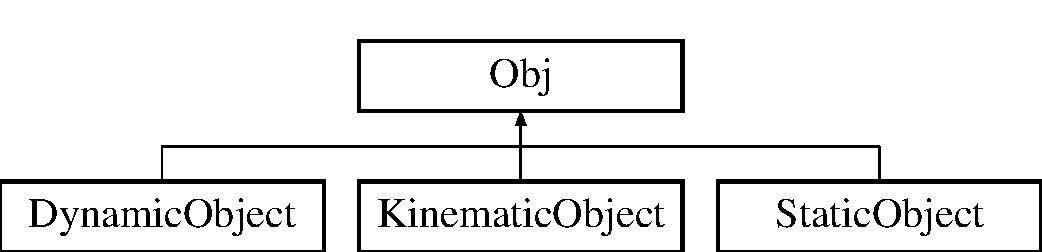
\includegraphics[height=2.000000cm]{class_obj}
\end{center}
\end{figure}
\subsection*{Public Attributes}
\begin{DoxyCompactItemize}
\item 
cp\+Body $\ast$ \hyperlink{class_obj_af55b595b6ea84887b090eabfd6f1eb4f}{body}\hypertarget{class_obj_af55b595b6ea84887b090eabfd6f1eb4f}{}\label{class_obj_af55b595b6ea84887b090eabfd6f1eb4f}

\begin{DoxyCompactList}\small\item\em Pointer to Chipmunk 2D body associated with the object. \end{DoxyCompactList}\item 
cp\+Shape $\ast$ \hyperlink{class_obj_ae16105e4cfa145f0dcd9fef57cebf01d}{shape}\hypertarget{class_obj_ae16105e4cfa145f0dcd9fef57cebf01d}{}\label{class_obj_ae16105e4cfa145f0dcd9fef57cebf01d}

\begin{DoxyCompactList}\small\item\em Pointer to Chipmunk 2D shape associated with the object. \end{DoxyCompactList}\item 
\hyperlink{class_obj_g_p_u_data}{Obj\+G\+P\+U\+Data} $\ast$ \hyperlink{class_obj_a33a9a5371319a410f7d2d395a7ef2423}{gpu\+Data}\hypertarget{class_obj_a33a9a5371319a410f7d2d395a7ef2423}{}\label{class_obj_a33a9a5371319a410f7d2d395a7ef2423}

\begin{DoxyCompactList}\small\item\em Pointer to the gpu data associated with the object. \end{DoxyCompactList}\item 
float \hyperlink{class_obj_ae3f4e1cecebf1ac2c5706fe4ddc3cd5b}{height}\hypertarget{class_obj_ae3f4e1cecebf1ac2c5706fe4ddc3cd5b}{}\label{class_obj_ae3f4e1cecebf1ac2c5706fe4ddc3cd5b}

\begin{DoxyCompactList}\small\item\em Height of the object. \end{DoxyCompactList}\item 
float \hyperlink{class_obj_ae91c4644ff64eb08a2d18dc1a9bbd315}{width}\hypertarget{class_obj_ae91c4644ff64eb08a2d18dc1a9bbd315}{}\label{class_obj_ae91c4644ff64eb08a2d18dc1a9bbd315}

\begin{DoxyCompactList}\small\item\em Width of the object. \end{DoxyCompactList}\item 
bool \hyperlink{class_obj_adf0f7b5c8ca61c7cfee46c832288fa19}{draw}\hypertarget{class_obj_adf0f7b5c8ca61c7cfee46c832288fa19}{}\label{class_obj_adf0f7b5c8ca61c7cfee46c832288fa19}

\begin{DoxyCompactList}\small\item\em Flag for whether the object should be drawn or not. \end{DoxyCompactList}\end{DoxyCompactItemize}


\subsection{Detailed Description}
The \hyperlink{class_obj}{Obj} class acts as a base class for static, dynamic, and kinematic objects. It holds the physics data (Chipmunk 2D) and gpu data of an object. 
\hypertarget{class_obj_g_p_u_data}{}\section{Obj\+G\+P\+U\+Data Class Reference}
\label{class_obj_g_p_u_data}\index{Obj\+G\+P\+U\+Data@{Obj\+G\+P\+U\+Data}}


{\ttfamily \#include $<$Obj\+G\+P\+U\+Data.\+h$>$}

\subsection*{Classes}
\begin{DoxyCompactItemize}
\item 
class {\bfseries Material}
\begin{DoxyCompactList}\small\item\em Class for storing material information loaded from .mtl file. \end{DoxyCompactList}\end{DoxyCompactItemize}
\subsection*{Public Types}
\begin{DoxyCompactItemize}
\item 
enum {\bfseries data\+Type} \+: short \hypertarget{class_obj_g_p_u_data_a3f9703333cd44735587ec9538ee700c1}{}\label{class_obj_g_p_u_data_a3f9703333cd44735587ec9538ee700c1}

\item 
enum {\bfseries mtl\+Data\+Type} \+: short \hypertarget{class_obj_g_p_u_data_a1707d7430f8c5e15d6d059378414017c}{}\label{class_obj_g_p_u_data_a1707d7430f8c5e15d6d059378414017c}

\end{DoxyCompactItemize}
\subsection*{Public Member Functions}
\begin{DoxyCompactItemize}
\item 
\hyperlink{class_obj_g_p_u_data_aec4780be6075400b351e25e75716bad2}{Obj\+G\+P\+U\+Data} (char $\ast$obj\+File, float angle=0.\+0f)
\begin{DoxyCompactList}\small\item\em \hyperlink{class_obj_g_p_u_data}{Obj\+G\+P\+U\+Data} constructor. \end{DoxyCompactList}\end{DoxyCompactItemize}
\subsection*{Public Attributes}
\begin{DoxyCompactItemize}
\item 
std\+::vector$<$ glm\+::vec3 $>$ \hyperlink{class_obj_g_p_u_data_a4479fbcb9ab78bd29f74d768d893123f}{v\+List}\hypertarget{class_obj_g_p_u_data_a4479fbcb9ab78bd29f74d768d893123f}{}\label{class_obj_g_p_u_data_a4479fbcb9ab78bd29f74d768d893123f}

\begin{DoxyCompactList}\small\item\em Stores vertex coordinates loaded from .obj file. \end{DoxyCompactList}\item 
std\+::vector$<$ glm\+::vec2 $>$ \hyperlink{class_obj_g_p_u_data_ab39012ed3e485641f2eda7c7f3de2aec}{v\+Texture\+List}\hypertarget{class_obj_g_p_u_data_ab39012ed3e485641f2eda7c7f3de2aec}{}\label{class_obj_g_p_u_data_ab39012ed3e485641f2eda7c7f3de2aec}

\begin{DoxyCompactList}\small\item\em Stores texture coordinates loaded from .obj file. \end{DoxyCompactList}\item 
std\+::vector$<$ glm\+::vec3 $>$ \hyperlink{class_obj_g_p_u_data_adc7cd78dfb5f2d69998fbdde2e77464f}{v\+Normal\+List}\hypertarget{class_obj_g_p_u_data_adc7cd78dfb5f2d69998fbdde2e77464f}{}\label{class_obj_g_p_u_data_adc7cd78dfb5f2d69998fbdde2e77464f}

\begin{DoxyCompactList}\small\item\em Stores vertex normals loaded from .obj file. \end{DoxyCompactList}\item 
std\+::vector$<$ G\+Luint $>$ \hyperlink{class_obj_g_p_u_data_a2672a6ddbbc6ed386477662f7970ce5f}{f\+List}\hypertarget{class_obj_g_p_u_data_a2672a6ddbbc6ed386477662f7970ce5f}{}\label{class_obj_g_p_u_data_a2672a6ddbbc6ed386477662f7970ce5f}

\begin{DoxyCompactList}\small\item\em Stores faces loaded from .obj file. \end{DoxyCompactList}\item 
std\+::vector$<$ int $>$ \hyperlink{class_obj_g_p_u_data_ab372a052982848b3f1b4d9b316d8d2b5}{material\+Indices}\hypertarget{class_obj_g_p_u_data_ab372a052982848b3f1b4d9b316d8d2b5}{}\label{class_obj_g_p_u_data_ab372a052982848b3f1b4d9b316d8d2b5}

\begin{DoxyCompactList}\small\item\em Marks divisions of different materials given in the .obj file (and defined in .mtl file) \end{DoxyCompactList}\item 
std\+::vector$<$ Material $>$ \hyperlink{class_obj_g_p_u_data_acfdaa154dbbb2b23512b4f65ec1ac708}{materials}\hypertarget{class_obj_g_p_u_data_acfdaa154dbbb2b23512b4f65ec1ac708}{}\label{class_obj_g_p_u_data_acfdaa154dbbb2b23512b4f65ec1ac708}

\begin{DoxyCompactList}\small\item\em Stores material information loaded from .mtl file. \end{DoxyCompactList}\item 
G\+Luint \hyperlink{class_obj_g_p_u_data_a723846f0ce483bd69094834e18e17e13}{vertex\+Array\+Obj}\hypertarget{class_obj_g_p_u_data_a723846f0ce483bd69094834e18e17e13}{}\label{class_obj_g_p_u_data_a723846f0ce483bd69094834e18e17e13}

\begin{DoxyCompactList}\small\item\em Name to bind the vertex array object. \end{DoxyCompactList}\item 
G\+Luint \hyperlink{class_obj_g_p_u_data_a64363bc12d8082f77948946d2542a89b}{element\+Buffer}\hypertarget{class_obj_g_p_u_data_a64363bc12d8082f77948946d2542a89b}{}\label{class_obj_g_p_u_data_a64363bc12d8082f77948946d2542a89b}

\begin{DoxyCompactList}\small\item\em Name to bind the element buffer object. \end{DoxyCompactList}\item 
G\+Luint \hyperlink{class_obj_g_p_u_data_ac89933479b0d8929860ee7317a4bdfdf}{vertex\+Buffer}\hypertarget{class_obj_g_p_u_data_ac89933479b0d8929860ee7317a4bdfdf}{}\label{class_obj_g_p_u_data_ac89933479b0d8929860ee7317a4bdfdf}

\begin{DoxyCompactList}\small\item\em Name to bind the vertex buffer object. \end{DoxyCompactList}\item 
G\+Luint \hyperlink{class_obj_g_p_u_data_aa35cf8a237a4b9a84156c880b534214a}{texture\+Buffer}\hypertarget{class_obj_g_p_u_data_aa35cf8a237a4b9a84156c880b534214a}{}\label{class_obj_g_p_u_data_aa35cf8a237a4b9a84156c880b534214a}

\begin{DoxyCompactList}\small\item\em Name to bind the texture coordinate buffer object. \end{DoxyCompactList}\item 
G\+Luint \hyperlink{class_obj_g_p_u_data_a3d56bdaa9f44c1c780761b0cd10f7dc3}{normal\+Buffer}\hypertarget{class_obj_g_p_u_data_a3d56bdaa9f44c1c780761b0cd10f7dc3}{}\label{class_obj_g_p_u_data_a3d56bdaa9f44c1c780761b0cd10f7dc3}

\begin{DoxyCompactList}\small\item\em Name to bind the vertex normal buffer object. \end{DoxyCompactList}\item 
glm\+::mat4 \hyperlink{class_obj_g_p_u_data_ac28a5f3da3cea8eaf4b4cc52596297fd}{unit\+Scale}\hypertarget{class_obj_g_p_u_data_ac28a5f3da3cea8eaf4b4cc52596297fd}{}\label{class_obj_g_p_u_data_ac28a5f3da3cea8eaf4b4cc52596297fd}

\begin{DoxyCompactList}\small\item\em Scaling factor to adjust object to size 1.\+0 in y-\/axis (height) \end{DoxyCompactList}\item 
glm\+::mat4 \hyperlink{class_obj_g_p_u_data_a208435c6c7c618dcf608e165297de85a}{rotation}\hypertarget{class_obj_g_p_u_data_a208435c6c7c618dcf608e165297de85a}{}\label{class_obj_g_p_u_data_a208435c6c7c618dcf608e165297de85a}

\begin{DoxyCompactList}\small\item\em Rotation about y-\/axis to adjust objects initial rotational centering (if required\+: this is what the optional constructor argument sets) \end{DoxyCompactList}\item 
float \hyperlink{class_obj_g_p_u_data_aa95922f6ad01e53e638ae6dd1fa698a5}{wh\+Ratio}\hypertarget{class_obj_g_p_u_data_aa95922f6ad01e53e638ae6dd1fa698a5}{}\label{class_obj_g_p_u_data_aa95922f6ad01e53e638ae6dd1fa698a5}

\begin{DoxyCompactList}\small\item\em Ratio of maximum x-\/axis vertex separation (width) to maximum y-\/axis vertex separation (height) \end{DoxyCompactList}\end{DoxyCompactItemize}
\subsection*{Private Member Functions}
\begin{DoxyCompactItemize}
\item 
void \hyperlink{class_obj_g_p_u_data_a5926e9755a614029b893f3ffa6147b43}{load\+Object} (char $\ast$file\+Name)
\begin{DoxyCompactList}\small\item\em Parses .obj and .mtl files and stores the data. \end{DoxyCompactList}\item 
data\+Type \hyperlink{class_obj_g_p_u_data_a9a006c8f431ffc2ee676e10a3cd0fe44}{get\+Data\+Type} (std\+::string data\+Type\+String)
\begin{DoxyCompactList}\small\item\em Converts string to .obj file datatype (data\+Type). \end{DoxyCompactList}\item 
mtl\+Data\+Type \hyperlink{class_obj_g_p_u_data_a3be542ac0e0ed9f7f34db0eae7346e49}{get\+Mtl\+Data\+Type} (std\+::string data\+Type\+String)
\begin{DoxyCompactList}\small\item\em Converts string to .mtl file datatype (mtl\+Data\+Type). \end{DoxyCompactList}\end{DoxyCompactItemize}


\subsection{Detailed Description}
The \hyperlink{class_obj_g_p_u_data}{Obj\+G\+P\+U\+Data} class loads and stores data used by the G\+PU to render objects. Each object is defined by three files which are loaded by this class\+: an object file (.obj) which contains information about vertices, faces, normals, and texture coordinates; a material file (.mtl) which contains texture and lighting information; and an image file(s) (.dds) which contain the texture images. 

\subsection{Constructor \& Destructor Documentation}
\index{Obj\+G\+P\+U\+Data@{Obj\+G\+P\+U\+Data}!Obj\+G\+P\+U\+Data@{Obj\+G\+P\+U\+Data}}
\index{Obj\+G\+P\+U\+Data@{Obj\+G\+P\+U\+Data}!Obj\+G\+P\+U\+Data@{Obj\+G\+P\+U\+Data}}
\subsubsection[{\texorpdfstring{Obj\+G\+P\+U\+Data(char $\ast$obj\+File, float angle=0.\+0f)}{ObjGPUData(char *objFile, float angle=0.0f)}}]{\setlength{\rightskip}{0pt plus 5cm}Obj\+G\+P\+U\+Data\+::\+Obj\+G\+P\+U\+Data (
\begin{DoxyParamCaption}
\item[{char $\ast$}]{obj\+File, }
\item[{float}]{angle = {\ttfamily 0.0f}}
\end{DoxyParamCaption}
)}\hypertarget{class_obj_g_p_u_data_aec4780be6075400b351e25e75716bad2}{}\label{class_obj_g_p_u_data_aec4780be6075400b351e25e75716bad2}


\hyperlink{class_obj_g_p_u_data}{Obj\+G\+P\+U\+Data} constructor. 


\begin{DoxyParams}{Parameters}
{\em obj\+File} & Object and material file path (these should have the same name) without extension \\
\hline
{\em angle} & Initial y-\/axis rotation in radians (optional\+: default 0.\+0) \\
\hline
\end{DoxyParams}


\subsection{Member Function Documentation}
\index{Obj\+G\+P\+U\+Data@{Obj\+G\+P\+U\+Data}!get\+Data\+Type@{get\+Data\+Type}}
\index{get\+Data\+Type@{get\+Data\+Type}!Obj\+G\+P\+U\+Data@{Obj\+G\+P\+U\+Data}}
\subsubsection[{\texorpdfstring{get\+Data\+Type(std\+::string data\+Type\+String)}{getDataType(std::string dataTypeString)}}]{\setlength{\rightskip}{0pt plus 5cm}Obj\+G\+P\+U\+Data\+::data\+Type Obj\+G\+P\+U\+Data\+::get\+Data\+Type (
\begin{DoxyParamCaption}
\item[{std\+::string}]{data\+Type\+String}
\end{DoxyParamCaption}
)\hspace{0.3cm}{\ttfamily [private]}}\hypertarget{class_obj_g_p_u_data_a9a006c8f431ffc2ee676e10a3cd0fe44}{}\label{class_obj_g_p_u_data_a9a006c8f431ffc2ee676e10a3cd0fe44}


Converts string to .obj file datatype (data\+Type). 


\begin{DoxyParams}{Parameters}
{\em data\+Type\+String} & The string to be converted. \\
\hline
\end{DoxyParams}
\begin{DoxyReturn}{Returns}
Equivalent data\+Type value. 
\end{DoxyReturn}
\index{Obj\+G\+P\+U\+Data@{Obj\+G\+P\+U\+Data}!get\+Mtl\+Data\+Type@{get\+Mtl\+Data\+Type}}
\index{get\+Mtl\+Data\+Type@{get\+Mtl\+Data\+Type}!Obj\+G\+P\+U\+Data@{Obj\+G\+P\+U\+Data}}
\subsubsection[{\texorpdfstring{get\+Mtl\+Data\+Type(std\+::string data\+Type\+String)}{getMtlDataType(std::string dataTypeString)}}]{\setlength{\rightskip}{0pt plus 5cm}Obj\+G\+P\+U\+Data\+::mtl\+Data\+Type Obj\+G\+P\+U\+Data\+::get\+Mtl\+Data\+Type (
\begin{DoxyParamCaption}
\item[{std\+::string}]{data\+Type\+String}
\end{DoxyParamCaption}
)\hspace{0.3cm}{\ttfamily [private]}}\hypertarget{class_obj_g_p_u_data_a3be542ac0e0ed9f7f34db0eae7346e49}{}\label{class_obj_g_p_u_data_a3be542ac0e0ed9f7f34db0eae7346e49}


Converts string to .mtl file datatype (mtl\+Data\+Type). 


\begin{DoxyParams}{Parameters}
{\em data\+Type\+String} & The string to be converted. \\
\hline
\end{DoxyParams}
\begin{DoxyReturn}{Returns}
Equivalent mtl\+Data\+Type value. 
\end{DoxyReturn}
\index{Obj\+G\+P\+U\+Data@{Obj\+G\+P\+U\+Data}!load\+Object@{load\+Object}}
\index{load\+Object@{load\+Object}!Obj\+G\+P\+U\+Data@{Obj\+G\+P\+U\+Data}}
\subsubsection[{\texorpdfstring{load\+Object(char $\ast$file\+Name)}{loadObject(char *fileName)}}]{\setlength{\rightskip}{0pt plus 5cm}void Obj\+G\+P\+U\+Data\+::load\+Object (
\begin{DoxyParamCaption}
\item[{char $\ast$}]{file\+Name}
\end{DoxyParamCaption}
)\hspace{0.3cm}{\ttfamily [private]}}\hypertarget{class_obj_g_p_u_data_a5926e9755a614029b893f3ffa6147b43}{}\label{class_obj_g_p_u_data_a5926e9755a614029b893f3ffa6147b43}


Parses .obj and .mtl files and stores the data. 


\begin{DoxyParams}{Parameters}
{\em file\+Name} & Name (without extension) of the .obj and .mtl files \\
\hline
\end{DoxyParams}

\hypertarget{class_obj_g_p_u_data_store}{}\section{Obj\+G\+P\+U\+Data\+Store Class Reference}
\label{class_obj_g_p_u_data_store}\index{Obj\+G\+P\+U\+Data\+Store@{Obj\+G\+P\+U\+Data\+Store}}


{\ttfamily \#include $<$Obj\+G\+P\+U\+Data\+Store.\+h$>$}

\subsection*{Public Member Functions}
\begin{DoxyCompactItemize}
\item 
\hyperlink{class_obj_g_p_u_data_store_a548c764aab1fe4fd622c924dd1c7eb89}{Obj\+G\+P\+U\+Data\+Store} ()\hypertarget{class_obj_g_p_u_data_store_a548c764aab1fe4fd622c924dd1c7eb89}{}\label{class_obj_g_p_u_data_store_a548c764aab1fe4fd622c924dd1c7eb89}

\begin{DoxyCompactList}\small\item\em Constructor. \end{DoxyCompactList}\item 
\hyperlink{class_obj_g_p_u_data}{Obj\+G\+P\+U\+Data} $\ast$ \hyperlink{class_obj_g_p_u_data_store_aa92191fb7db9147b05e89c983bf294db}{add} (std\+::string path, float angle=0.\+0, bool scaling\+Mode=true)
\begin{DoxyCompactList}\small\item\em Adds a new mesh/texture to the store\+: if not in the store, it loads and stores; if already present, it does nothing. \end{DoxyCompactList}\item 
\hyperlink{class_obj_g_p_u_data}{Obj\+G\+P\+U\+Data} $\ast$ \hyperlink{class_obj_g_p_u_data_store_a3b54d794f6aaa9cd1478934b018d47e9}{get} (std\+::string path)
\begin{DoxyCompactList}\small\item\em Retrieves gpu data from the store. \end{DoxyCompactList}\end{DoxyCompactItemize}
\subsection*{Private Attributes}
\begin{DoxyCompactItemize}
\item 
std\+::map$<$ std\+::string, \hyperlink{class_obj_g_p_u_data}{Obj\+G\+P\+U\+Data} $\ast$ $>$ \hyperlink{class_obj_g_p_u_data_store_a3872d9f1ae3877eafd8b068c3aba4694}{gpu\+Map}\hypertarget{class_obj_g_p_u_data_store_a3872d9f1ae3877eafd8b068c3aba4694}{}\label{class_obj_g_p_u_data_store_a3872d9f1ae3877eafd8b068c3aba4694}

\begin{DoxyCompactList}\small\item\em Map translates object file name to stored data. \end{DoxyCompactList}\end{DoxyCompactItemize}


\subsection{Detailed Description}
The \hyperlink{class_obj_g_p_u_data_store}{Obj\+G\+P\+U\+Data\+Store} class acts as a storage class for loaded object mesh/texture data. 

\subsection{Member Function Documentation}
\index{Obj\+G\+P\+U\+Data\+Store@{Obj\+G\+P\+U\+Data\+Store}!add@{add}}
\index{add@{add}!Obj\+G\+P\+U\+Data\+Store@{Obj\+G\+P\+U\+Data\+Store}}
\subsubsection[{\texorpdfstring{add(std\+::string path, float angle=0.\+0, bool scaling\+Mode=true)}{add(std::string path, float angle=0.0, bool scalingMode=true)}}]{\setlength{\rightskip}{0pt plus 5cm}{\bf Obj\+G\+P\+U\+Data}$\ast$ Obj\+G\+P\+U\+Data\+Store\+::add (
\begin{DoxyParamCaption}
\item[{std\+::string}]{path, }
\item[{float}]{angle = {\ttfamily 0.0}, }
\item[{bool}]{scaling\+Mode = {\ttfamily true}}
\end{DoxyParamCaption}
)}\hypertarget{class_obj_g_p_u_data_store_aa92191fb7db9147b05e89c983bf294db}{}\label{class_obj_g_p_u_data_store_aa92191fb7db9147b05e89c983bf294db}


Adds a new mesh/texture to the store\+: if not in the store, it loads and stores; if already present, it does nothing. 


\begin{DoxyParams}{Parameters}
{\em path} & Path to object file \\
\hline
{\em angle} & Initial y-\/axis rotation in radians (optional\+: default 0.\+0) \\
\hline
{\em scaling\+Mode} & Flag specifies if object should be scaled to unit height when loaded (default true) \\
\hline
\end{DoxyParams}
\index{Obj\+G\+P\+U\+Data\+Store@{Obj\+G\+P\+U\+Data\+Store}!get@{get}}
\index{get@{get}!Obj\+G\+P\+U\+Data\+Store@{Obj\+G\+P\+U\+Data\+Store}}
\subsubsection[{\texorpdfstring{get(std\+::string path)}{get(std::string path)}}]{\setlength{\rightskip}{0pt plus 5cm}{\bf Obj\+G\+P\+U\+Data}$\ast$ Obj\+G\+P\+U\+Data\+Store\+::get (
\begin{DoxyParamCaption}
\item[{std\+::string}]{path}
\end{DoxyParamCaption}
)}\hypertarget{class_obj_g_p_u_data_store_a3b54d794f6aaa9cd1478934b018d47e9}{}\label{class_obj_g_p_u_data_store_a3b54d794f6aaa9cd1478934b018d47e9}


Retrieves gpu data from the store. 


\begin{DoxyParams}{Parameters}
{\em path} & Path to object file to search for \\
\hline
\end{DoxyParams}


The documentation for this class was generated from the following file\+:\begin{DoxyCompactItemize}
\item 
Obj\+G\+P\+U\+Data\+Store.\+h\end{DoxyCompactItemize}

\hypertarget{class_physics_object}{}\section{Physics\+Object Class Reference}
\label{class_physics_object}\index{Physics\+Object@{Physics\+Object}}


{\ttfamily \#include $<$Physics\+Object.\+h$>$}



Inheritance diagram for Physics\+Object\+:
\nopagebreak
\begin{figure}[H]
\begin{center}
\leavevmode
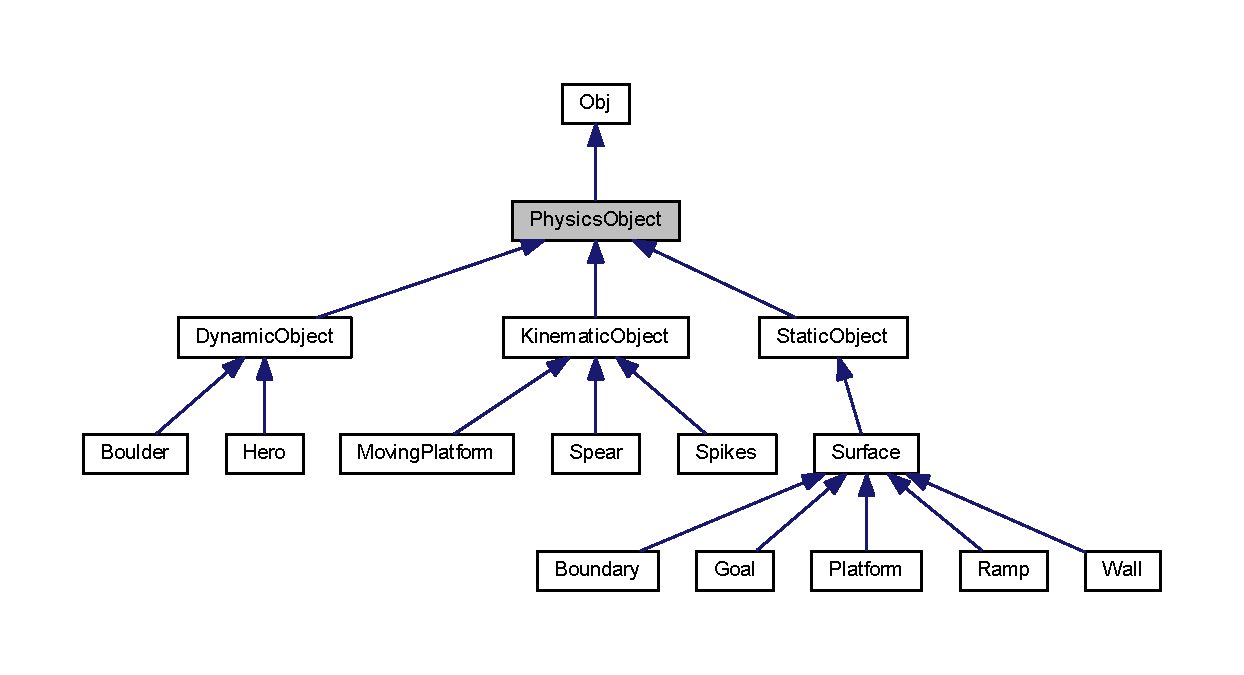
\includegraphics[width=350pt]{class_physics_object__inherit__graph}
\end{center}
\end{figure}


Collaboration diagram for Physics\+Object\+:
\nopagebreak
\begin{figure}[H]
\begin{center}
\leavevmode
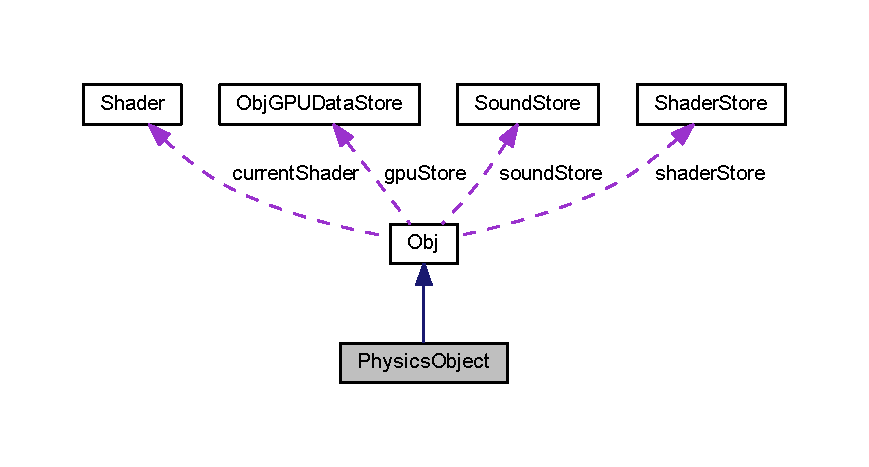
\includegraphics[width=350pt]{class_physics_object__coll__graph}
\end{center}
\end{figure}
\subsection*{Public Member Functions}
\begin{DoxyCompactItemize}
\item 
virtual \hyperlink{class_physics_object_ade6588d8622cff10e979118e0f8a076e}{$\sim$\+Physics\+Object} ()\hypertarget{class_physics_object_ade6588d8622cff10e979118e0f8a076e}{}\label{class_physics_object_ade6588d8622cff10e979118e0f8a076e}

\begin{DoxyCompactList}\small\item\em \hyperlink{class_physics_object}{Physics\+Object} constructor. \end{DoxyCompactList}\item 
void \hyperlink{class_physics_object_a37fcb312275149e32e30ade97c30ff8d}{render} ()\hypertarget{class_physics_object_a37fcb312275149e32e30ade97c30ff8d}{}\label{class_physics_object_a37fcb312275149e32e30ade97c30ff8d}

\begin{DoxyCompactList}\small\item\em Renders the object. \end{DoxyCompactList}\end{DoxyCompactItemize}
\subsection*{Public Attributes}
\begin{DoxyCompactItemize}
\item 
cp\+Body $\ast$ \hyperlink{class_physics_object_ae836920d09d47b9b046c69c3fdd8dba1}{body}\hypertarget{class_physics_object_ae836920d09d47b9b046c69c3fdd8dba1}{}\label{class_physics_object_ae836920d09d47b9b046c69c3fdd8dba1}

\begin{DoxyCompactList}\small\item\em Pointer to Chipmunk 2D body associated with the object. \end{DoxyCompactList}\item 
cp\+Shape $\ast$ \hyperlink{class_physics_object_a1c41c18cdfe7fababf08210dd36c4d52}{shape}\hypertarget{class_physics_object_a1c41c18cdfe7fababf08210dd36c4d52}{}\label{class_physics_object_a1c41c18cdfe7fababf08210dd36c4d52}

\begin{DoxyCompactList}\small\item\em Pointer to Chipmunk 2D shape associated with the object. \end{DoxyCompactList}\item 
cp\+Vect \hyperlink{class_physics_object_a732744541b96297fe68bcdd4eb15eadc}{standing\+Normal}\hypertarget{class_physics_object_a732744541b96297fe68bcdd4eb15eadc}{}\label{class_physics_object_a732744541b96297fe68bcdd4eb15eadc}

\begin{DoxyCompactList}\small\item\em Normal used in collision handler to determine if hero can jump. \end{DoxyCompactList}\item 
cp\+Vect \hyperlink{class_physics_object_ad4320fa83060bd24c85e5f7a06d07650}{death\+Normal}\hypertarget{class_physics_object_ad4320fa83060bd24c85e5f7a06d07650}{}\label{class_physics_object_ad4320fa83060bd24c85e5f7a06d07650}

\begin{DoxyCompactList}\small\item\em Normal used in collision handler to determine if hero should be killed. \end{DoxyCompactList}\end{DoxyCompactItemize}
\subsection*{Static Public Attributes}
\begin{DoxyCompactItemize}
\item 
static cp\+Space $\ast$ \hyperlink{class_physics_object_af51d68e507cb0a7796241695b1c78046}{space}\hypertarget{class_physics_object_af51d68e507cb0a7796241695b1c78046}{}\label{class_physics_object_af51d68e507cb0a7796241695b1c78046}

\begin{DoxyCompactList}\small\item\em Pointer to current Chipmunk 2D space. \end{DoxyCompactList}\end{DoxyCompactItemize}


\subsection{Detailed Description}
The \hyperlink{class_physics_object}{Physics\+Object} class is derived from the \hyperlink{class_obj}{Obj} class and is the parent to all objects associated with Chipmunk2D. 

The documentation for this class was generated from the following file\+:\begin{DoxyCompactItemize}
\item 
Physics\+Object.\+h\end{DoxyCompactItemize}

\hypertarget{class_platform}{}\section{Platform Class Reference}
\label{class_platform}\index{Platform@{Platform}}


{\ttfamily \#include $<$Platform.\+h$>$}



Inheritance diagram for Platform\+:
\nopagebreak
\begin{figure}[H]
\begin{center}
\leavevmode
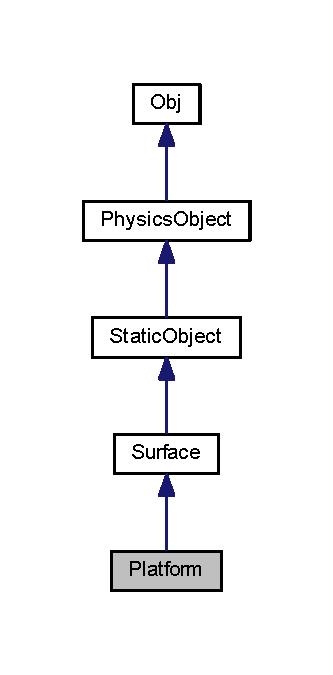
\includegraphics[width=160pt]{class_platform__inherit__graph}
\end{center}
\end{figure}


Collaboration diagram for Platform\+:
\nopagebreak
\begin{figure}[H]
\begin{center}
\leavevmode
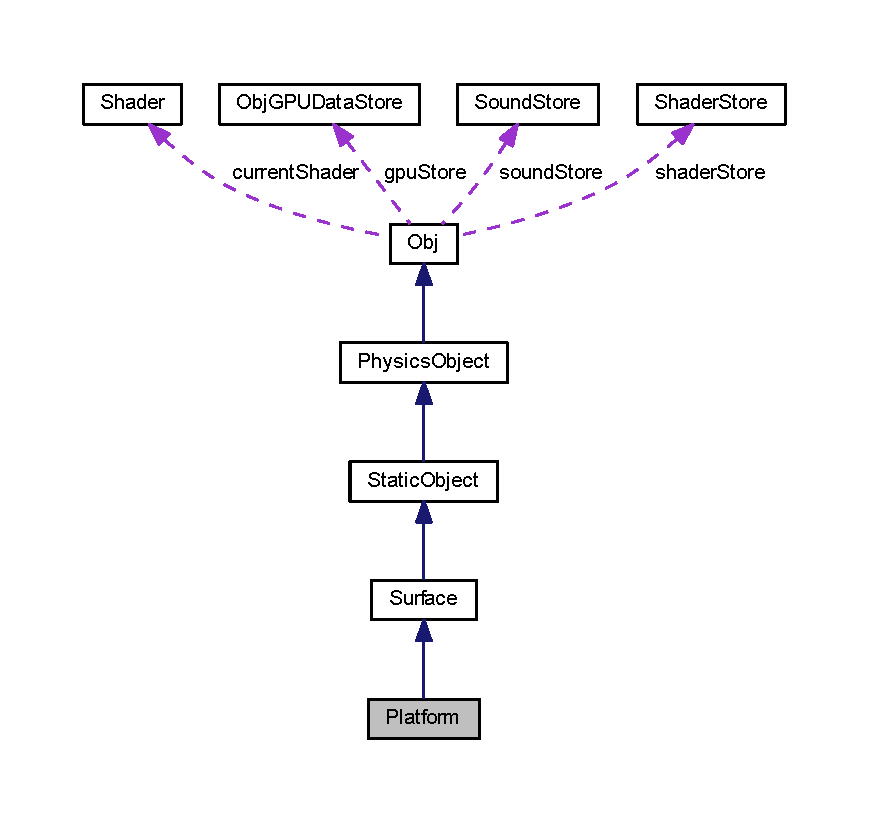
\includegraphics[width=350pt]{class_platform__coll__graph}
\end{center}
\end{figure}
\subsection*{Public Member Functions}
\begin{DoxyCompactItemize}
\item 
\hyperlink{class_platform_a269dd00d537d8c3622738e3dac1e9afa}{Platform} (float x1, float x2, float ymid, float thickness=50.\+0f)
\begin{DoxyCompactList}\small\item\em \hyperlink{class_platform}{Platform} constructor. \end{DoxyCompactList}\end{DoxyCompactItemize}
\subsection*{Additional Inherited Members}


\subsection{Detailed Description}
The \hyperlink{class_platform}{Platform} class implements platform objects. 

\subsection{Constructor \& Destructor Documentation}
\index{Platform@{Platform}!Platform@{Platform}}
\index{Platform@{Platform}!Platform@{Platform}}
\subsubsection[{\texorpdfstring{Platform(float x1, float x2, float ymid, float thickness=50.\+0f)}{Platform(float x1, float x2, float ymid, float thickness=50.0f)}}]{\setlength{\rightskip}{0pt plus 5cm}Platform\+::\+Platform (
\begin{DoxyParamCaption}
\item[{float}]{x1, }
\item[{float}]{x2, }
\item[{float}]{ymid, }
\item[{float}]{thickness = {\ttfamily 50.0f}}
\end{DoxyParamCaption}
)}\hypertarget{class_platform_a269dd00d537d8c3622738e3dac1e9afa}{}\label{class_platform_a269dd00d537d8c3622738e3dac1e9afa}


\hyperlink{class_platform}{Platform} constructor. 


\begin{DoxyParams}{Parameters}
{\em x1} & The leftmost extent of the platform. \\
\hline
{\em x2} & The rightmost extent of the platform. \\
\hline
{\em ymid} & The y-\/coordinate of the platform. \\
\hline
{\em thickness} & The vertical thickness of the platform (default = 50.\+0). \\
\hline
\end{DoxyParams}


The documentation for this class was generated from the following file\+:\begin{DoxyCompactItemize}
\item 
Platform.\+h\end{DoxyCompactItemize}

\hypertarget{class_ramp}{}\section{Ramp Class Reference}
\label{class_ramp}\index{Ramp@{Ramp}}


{\ttfamily \#include $<$Ramp.\+h$>$}



Inheritance diagram for Ramp\+:
\nopagebreak
\begin{figure}[H]
\begin{center}
\leavevmode
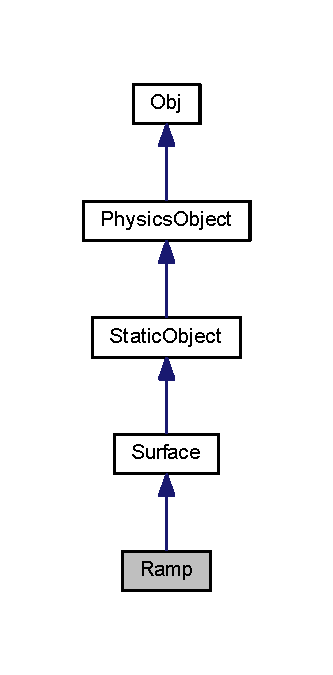
\includegraphics[width=160pt]{class_ramp__inherit__graph}
\end{center}
\end{figure}


Collaboration diagram for Ramp\+:
\nopagebreak
\begin{figure}[H]
\begin{center}
\leavevmode
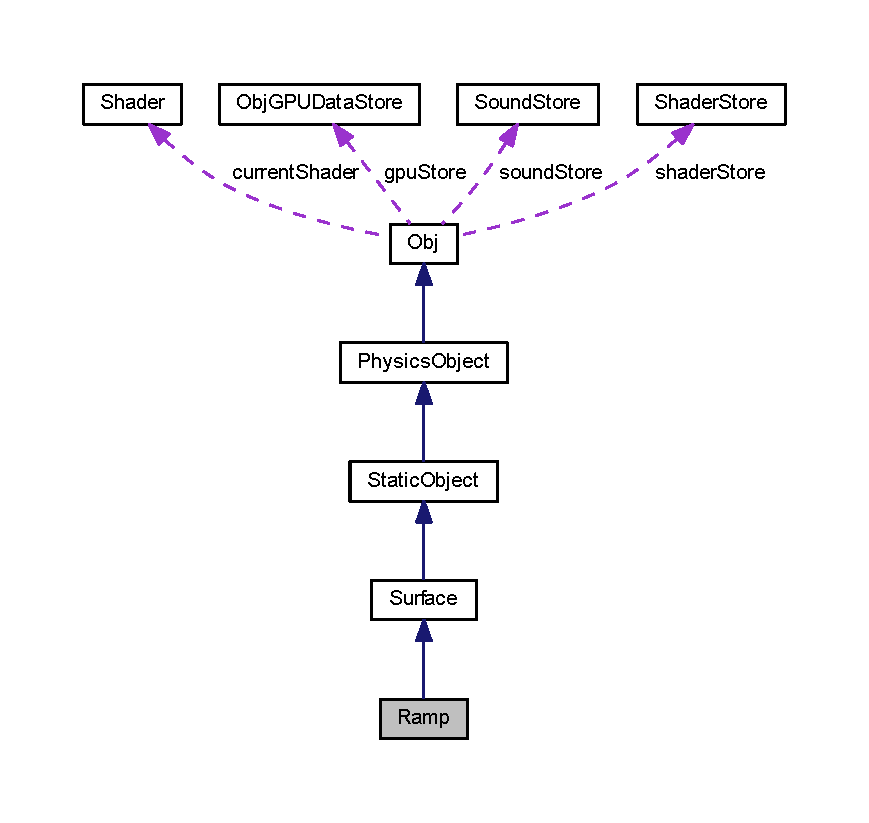
\includegraphics[width=350pt]{class_ramp__coll__graph}
\end{center}
\end{figure}
\subsection*{Public Member Functions}
\begin{DoxyCompactItemize}
\item 
\hyperlink{class_ramp_a5d012743839773fbb8cf51c848816fe4}{Ramp} (float x1, float x2, float y1, float y2, float thickness=50.\+0f)
\begin{DoxyCompactList}\small\item\em \hyperlink{class_ramp}{Ramp} constructor. \end{DoxyCompactList}\end{DoxyCompactItemize}
\subsection*{Additional Inherited Members}


\subsection{Detailed Description}
The \hyperlink{class_ramp}{Ramp} class implements ramp objects. 

\subsection{Constructor \& Destructor Documentation}
\index{Ramp@{Ramp}!Ramp@{Ramp}}
\index{Ramp@{Ramp}!Ramp@{Ramp}}
\subsubsection[{\texorpdfstring{Ramp(float x1, float x2, float y1, float y2, float thickness=50.\+0f)}{Ramp(float x1, float x2, float y1, float y2, float thickness=50.0f)}}]{\setlength{\rightskip}{0pt plus 5cm}Ramp\+::\+Ramp (
\begin{DoxyParamCaption}
\item[{float}]{x1, }
\item[{float}]{x2, }
\item[{float}]{y1, }
\item[{float}]{y2, }
\item[{float}]{thickness = {\ttfamily 50.0f}}
\end{DoxyParamCaption}
)}\hypertarget{class_ramp_a5d012743839773fbb8cf51c848816fe4}{}\label{class_ramp_a5d012743839773fbb8cf51c848816fe4}


\hyperlink{class_ramp}{Ramp} constructor. 


\begin{DoxyParams}{Parameters}
{\em x1} & The leftmost extent of the ramp. \\
\hline
{\em x2} & The rightmost extent of the ramp. \\
\hline
{\em y1} & The bottom y-\/coordinate of the ramp. \\
\hline
{\em y2} & The top y-\/coordinate of the ramp. \\
\hline
{\em thickness} & The thickness of the ramp (default = 50.\+0). \\
\hline
\end{DoxyParams}


The documentation for this class was generated from the following file\+:\begin{DoxyCompactItemize}
\item 
Ramp.\+h\end{DoxyCompactItemize}

\hypertarget{class_shader}{}\section{Shader Class Reference}
\label{class_shader}\index{Shader@{Shader}}


{\ttfamily \#include $<$Shader.\+h$>$}

\subsection*{Public Member Functions}
\begin{DoxyCompactItemize}
\item 
\hyperlink{class_shader_a6f5fe628c8b29e8d6c81595774951b6c}{Shader} (const char $\ast$v\+Shader, const char $\ast$f\+Shader)
\begin{DoxyCompactList}\small\item\em \hyperlink{class_shader}{Shader} constructor. \end{DoxyCompactList}\end{DoxyCompactItemize}
\subsection*{Public Attributes}
\begin{DoxyCompactItemize}
\item 
G\+Luint \hyperlink{class_shader_acd931b86aee746b644913712e0882940}{shader\+Program}\hypertarget{class_shader_acd931b86aee746b644913712e0882940}{}\label{class_shader_acd931b86aee746b644913712e0882940}

\begin{DoxyCompactList}\small\item\em Name to bind the shader program. \end{DoxyCompactList}\item 
std\+::map$<$ std\+::string, G\+Luint $>$ \hyperlink{class_shader_ad9404aed9f1d09a68b9bff126221cb90}{uniform\+I\+D\+Map}\hypertarget{class_shader_ad9404aed9f1d09a68b9bff126221cb90}{}\label{class_shader_ad9404aed9f1d09a68b9bff126221cb90}

\begin{DoxyCompactList}\small\item\em Stores names which bind the shader uniform I\+Ds. \end{DoxyCompactList}\end{DoxyCompactItemize}


\subsection{Detailed Description}
The \hyperlink{class_shader}{Shader} class is used to build shaders. All of the names/identifiers required to bind/use the shader afterwards are stored. 

\subsection{Constructor \& Destructor Documentation}
\index{Shader@{Shader}!Shader@{Shader}}
\index{Shader@{Shader}!Shader@{Shader}}
\subsubsection[{\texorpdfstring{Shader(const char $\ast$v\+Shader, const char $\ast$f\+Shader)}{Shader(const char *vShader, const char *fShader)}}]{\setlength{\rightskip}{0pt plus 5cm}Shader\+::\+Shader (
\begin{DoxyParamCaption}
\item[{const char $\ast$}]{v\+Shader, }
\item[{const char $\ast$}]{f\+Shader}
\end{DoxyParamCaption}
)}\hypertarget{class_shader_a6f5fe628c8b29e8d6c81595774951b6c}{}\label{class_shader_a6f5fe628c8b29e8d6c81595774951b6c}


\hyperlink{class_shader}{Shader} constructor. 


\begin{DoxyParams}{Parameters}
{\em v\+Shader} & Vertex shader path \\
\hline
{\em f\+Shader} & Fragment shader path \\
\hline
\end{DoxyParams}


The documentation for this class was generated from the following file\+:\begin{DoxyCompactItemize}
\item 
Shader.\+h\end{DoxyCompactItemize}

\hypertarget{class_shader_store}{}\section{Shader\+Store Class Reference}
\label{class_shader_store}\index{Shader\+Store@{Shader\+Store}}


{\ttfamily \#include $<$Shader\+Store.\+h$>$}

\subsection*{Public Member Functions}
\begin{DoxyCompactItemize}
\item 
\hyperlink{class_shader_store_acfd6bbef381749aa2d5d0efa6f176a14}{Shader\+Store} ()\hypertarget{class_shader_store_acfd6bbef381749aa2d5d0efa6f176a14}{}\label{class_shader_store_acfd6bbef381749aa2d5d0efa6f176a14}

\begin{DoxyCompactList}\small\item\em Constructor. \end{DoxyCompactList}\item 
\hyperlink{class_shader}{Shader} $\ast$ \hyperlink{class_shader_store_a05d990118a05385a515c06d50ee2843f}{add} (std\+::string vpath, std\+::string fpath)
\begin{DoxyCompactList}\small\item\em Adds a new shader to the store\+: if not in the store, it loads and stores; if already present, it does nothing. \end{DoxyCompactList}\item 
\hyperlink{class_shader}{Shader} $\ast$ \hyperlink{class_shader_store_ab4d641d0e399f7a4ca47a74f5ab4d66e}{get} (std\+::string vpath, std\+::string fpath)
\begin{DoxyCompactList}\small\item\em Retrieves gpu data from the store. \end{DoxyCompactList}\end{DoxyCompactItemize}
\subsection*{Private Attributes}
\begin{DoxyCompactItemize}
\item 
std\+::map$<$ std\+::string, \hyperlink{class_shader}{Shader} $\ast$ $>$ \hyperlink{class_shader_store_a23586974751c0c4fc9ce52eb3fa42985}{shader\+Map}\hypertarget{class_shader_store_a23586974751c0c4fc9ce52eb3fa42985}{}\label{class_shader_store_a23586974751c0c4fc9ce52eb3fa42985}

\begin{DoxyCompactList}\small\item\em Map translates sound file name to shader. \end{DoxyCompactList}\end{DoxyCompactItemize}


\subsection{Detailed Description}
The \hyperlink{class_shader_store}{Shader\+Store} class acts as a storage class for loaded shaders. 

\subsection{Member Function Documentation}
\index{Shader\+Store@{Shader\+Store}!add@{add}}
\index{add@{add}!Shader\+Store@{Shader\+Store}}
\subsubsection[{\texorpdfstring{add(std\+::string vpath, std\+::string fpath)}{add(std::string vpath, std::string fpath)}}]{\setlength{\rightskip}{0pt plus 5cm}{\bf Shader}$\ast$ Shader\+Store\+::add (
\begin{DoxyParamCaption}
\item[{std\+::string}]{vpath, }
\item[{std\+::string}]{fpath}
\end{DoxyParamCaption}
)}\hypertarget{class_shader_store_a05d990118a05385a515c06d50ee2843f}{}\label{class_shader_store_a05d990118a05385a515c06d50ee2843f}


Adds a new shader to the store\+: if not in the store, it loads and stores; if already present, it does nothing. 


\begin{DoxyParams}{Parameters}
{\em vpath} & Path to vertex shader \\
\hline
{\em fpath} & Path to fragment shader \\
\hline
\end{DoxyParams}
\index{Shader\+Store@{Shader\+Store}!get@{get}}
\index{get@{get}!Shader\+Store@{Shader\+Store}}
\subsubsection[{\texorpdfstring{get(std\+::string vpath, std\+::string fpath)}{get(std::string vpath, std::string fpath)}}]{\setlength{\rightskip}{0pt plus 5cm}{\bf Shader}$\ast$ Shader\+Store\+::get (
\begin{DoxyParamCaption}
\item[{std\+::string}]{vpath, }
\item[{std\+::string}]{fpath}
\end{DoxyParamCaption}
)}\hypertarget{class_shader_store_ab4d641d0e399f7a4ca47a74f5ab4d66e}{}\label{class_shader_store_ab4d641d0e399f7a4ca47a74f5ab4d66e}


Retrieves gpu data from the store. 


\begin{DoxyParams}{Parameters}
{\em vpath} & Path to vertex shader \\
\hline
{\em fpath} & Path to fragment shader \\
\hline
\end{DoxyParams}


The documentation for this class was generated from the following file\+:\begin{DoxyCompactItemize}
\item 
Shader\+Store.\+h\end{DoxyCompactItemize}

\hypertarget{class_skybox}{}\section{Skybox Class Reference}
\label{class_skybox}\index{Skybox@{Skybox}}


{\ttfamily \#include $<$Skybox.\+h$>$}



Inheritance diagram for Skybox\+:
\nopagebreak
\begin{figure}[H]
\begin{center}
\leavevmode
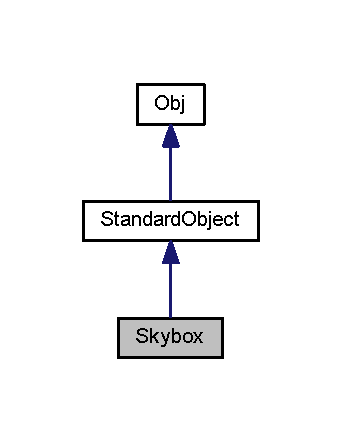
\includegraphics[width=164pt]{class_skybox__inherit__graph}
\end{center}
\end{figure}


Collaboration diagram for Skybox\+:
\nopagebreak
\begin{figure}[H]
\begin{center}
\leavevmode
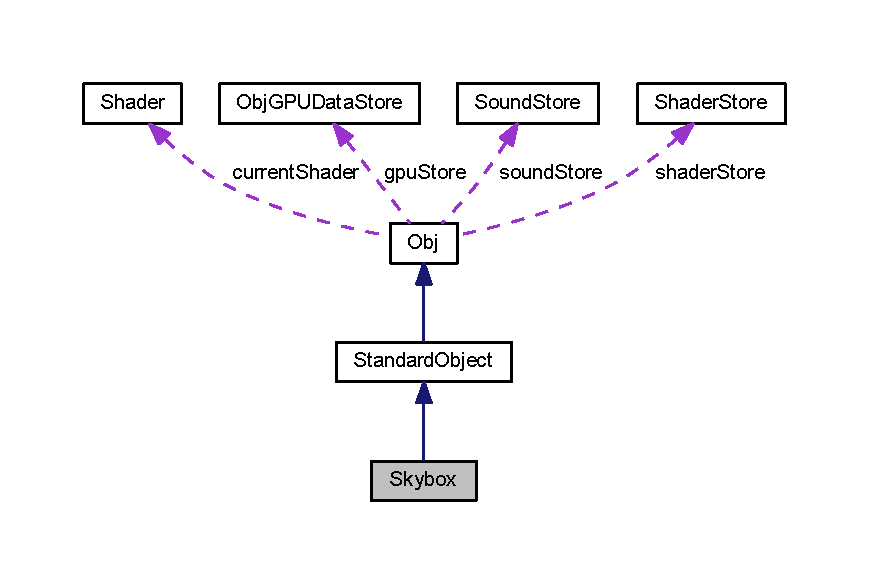
\includegraphics[width=350pt]{class_skybox__coll__graph}
\end{center}
\end{figure}
\subsection*{Public Member Functions}
\begin{DoxyCompactItemize}
\item 
\hyperlink{class_skybox_a1dd65128d43007cd91fea9917f4b00f4}{Skybox} (float x, float y, int bg\+Num)
\begin{DoxyCompactList}\small\item\em \hyperlink{class_skybox}{Skybox} constructor. \end{DoxyCompactList}\end{DoxyCompactItemize}
\subsection*{Additional Inherited Members}


\subsection{Detailed Description}
The \hyperlink{class_skybox}{Skybox} class implements the skybox used to provide the backdrop of the stage. 

\subsection{Constructor \& Destructor Documentation}
\index{Skybox@{Skybox}!Skybox@{Skybox}}
\index{Skybox@{Skybox}!Skybox@{Skybox}}
\subsubsection[{\texorpdfstring{Skybox(float x, float y, int bg\+Num)}{Skybox(float x, float y, int bgNum)}}]{\setlength{\rightskip}{0pt plus 5cm}Skybox\+::\+Skybox (
\begin{DoxyParamCaption}
\item[{float}]{x, }
\item[{float}]{y, }
\item[{int}]{bg\+Num}
\end{DoxyParamCaption}
)}\hypertarget{class_skybox_a1dd65128d43007cd91fea9917f4b00f4}{}\label{class_skybox_a1dd65128d43007cd91fea9917f4b00f4}


\hyperlink{class_skybox}{Skybox} constructor. 


\begin{DoxyParams}{Parameters}
{\em x} & The x coordinate of the skybox. \\
\hline
{\em y} & The y coordinate of the skybox. \\
\hline
{\em bg\+Num} & Int corresponding to the desired backdrop. \\
\hline
\end{DoxyParams}


The documentation for this class was generated from the following file\+:\begin{DoxyCompactItemize}
\item 
Skybox.\+h\end{DoxyCompactItemize}

\hypertarget{class_sound}{}\section{Sound Class Reference}
\label{class_sound}\index{Sound@{Sound}}


{\ttfamily \#include $<$Sound.\+h$>$}

\subsection*{Public Member Functions}
\begin{DoxyCompactItemize}
\item 
\hyperlink{class_sound_a77d59da64652f107b972f7dd5e468c5d}{Sound} (std\+::string path)
\begin{DoxyCompactList}\small\item\em \hyperlink{class_sound}{Sound} constructor. \end{DoxyCompactList}\item 
\hyperlink{class_sound_a0907389078bf740be2a5763366ad3376}{$\sim$\+Sound} ()\hypertarget{class_sound_a0907389078bf740be2a5763366ad3376}{}\label{class_sound_a0907389078bf740be2a5763366ad3376}

\begin{DoxyCompactList}\small\item\em \hyperlink{class_sound}{Sound} destructor. \end{DoxyCompactList}\item 
void \hyperlink{class_sound_a8705e3cb2a6407365cd6155bab713a1c}{play} (int loop=0)\hypertarget{class_sound_a8705e3cb2a6407365cd6155bab713a1c}{}\label{class_sound_a8705e3cb2a6407365cd6155bab713a1c}

\begin{DoxyCompactList}\small\item\em Plays the sound data contained in the class. \end{DoxyCompactList}\item 
void \hyperlink{class_sound_a07c551ab56d2f83a861a2f7fd81b480a}{stop} ()\hypertarget{class_sound_a07c551ab56d2f83a861a2f7fd81b480a}{}\label{class_sound_a07c551ab56d2f83a861a2f7fd81b480a}

\begin{DoxyCompactList}\small\item\em Stops playing sound. \end{DoxyCompactList}\end{DoxyCompactItemize}
\subsection*{Private Attributes}
\begin{DoxyCompactItemize}
\item 
A\+Luint \hyperlink{class_sound_abb059a11593afdbaa0b0682daf453bd0}{audio\+Buffer}\hypertarget{class_sound_abb059a11593afdbaa0b0682daf453bd0}{}\label{class_sound_abb059a11593afdbaa0b0682daf453bd0}

\begin{DoxyCompactList}\small\item\em Binding id for sound data storage. \end{DoxyCompactList}\item 
A\+Luint \hyperlink{class_sound_a17cbdf208c4c6a0cfe34ce80aa2c297d}{audio\+Source}\hypertarget{class_sound_a17cbdf208c4c6a0cfe34ce80aa2c297d}{}\label{class_sound_a17cbdf208c4c6a0cfe34ce80aa2c297d}

\begin{DoxyCompactList}\small\item\em Binding id for position, velocity, etc. of sound source. \end{DoxyCompactList}\item 
bool \hyperlink{class_sound_a4f97159af2e1cc951d21129202bfcbca}{loaded}\hypertarget{class_sound_a4f97159af2e1cc951d21129202bfcbca}{}\label{class_sound_a4f97159af2e1cc951d21129202bfcbca}

\begin{DoxyCompactList}\small\item\em Flag specifies if sound is loaded. \end{DoxyCompactList}\end{DoxyCompactItemize}


\subsection{Detailed Description}
The \hyperlink{class_sound}{Sound} class loads and stores sound data. 

\subsection{Constructor \& Destructor Documentation}
\index{Sound@{Sound}!Sound@{Sound}}
\index{Sound@{Sound}!Sound@{Sound}}
\subsubsection[{\texorpdfstring{Sound(std\+::string path)}{Sound(std::string path)}}]{\setlength{\rightskip}{0pt plus 5cm}Sound\+::\+Sound (
\begin{DoxyParamCaption}
\item[{std\+::string}]{path}
\end{DoxyParamCaption}
)}\hypertarget{class_sound_a77d59da64652f107b972f7dd5e468c5d}{}\label{class_sound_a77d59da64652f107b972f7dd5e468c5d}


\hyperlink{class_sound}{Sound} constructor. 


\begin{DoxyParams}{Parameters}
{\em path} & Path to the sound file that should be loaded. \\
\hline
\end{DoxyParams}


The documentation for this class was generated from the following file\+:\begin{DoxyCompactItemize}
\item 
Sound.\+h\end{DoxyCompactItemize}

\hypertarget{class_sound_store}{}\section{Sound\+Store Class Reference}
\label{class_sound_store}\index{Sound\+Store@{Sound\+Store}}


{\ttfamily \#include $<$Sound\+Store.\+h$>$}

\subsection*{Public Member Functions}
\begin{DoxyCompactItemize}
\item 
\hyperlink{class_sound_store_a14e85794e6633aa83dbab0b1cb72826a}{Sound\+Store} ()\hypertarget{class_sound_store_a14e85794e6633aa83dbab0b1cb72826a}{}\label{class_sound_store_a14e85794e6633aa83dbab0b1cb72826a}

\begin{DoxyCompactList}\small\item\em Constructor. \end{DoxyCompactList}\item 
\hyperlink{class_sound}{Sound} $\ast$ \hyperlink{class_sound_store_acad2fc70afd94cb00618e3bbea29976c}{add} (std\+::string path)
\begin{DoxyCompactList}\small\item\em Adds a new sound to the store\+: if not in the store, it loads and stores; if already present, it does nothing. \end{DoxyCompactList}\item 
\hyperlink{class_sound}{Sound} $\ast$ \hyperlink{class_sound_store_a5694dfe7d0a1d4d10b6a6aa6d7828a92}{get} (std\+::string path)
\begin{DoxyCompactList}\small\item\em Retrieves gpu data from the store. \end{DoxyCompactList}\end{DoxyCompactItemize}
\subsection*{Private Attributes}
\begin{DoxyCompactItemize}
\item 
std\+::map$<$ std\+::string, \hyperlink{class_sound}{Sound} $\ast$ $>$ \hyperlink{class_sound_store_a33cb077cb9c34febb095fc3a528db0a5}{sound\+Map}\hypertarget{class_sound_store_a33cb077cb9c34febb095fc3a528db0a5}{}\label{class_sound_store_a33cb077cb9c34febb095fc3a528db0a5}

\begin{DoxyCompactList}\small\item\em Map translates sound file name to stored data. \end{DoxyCompactList}\end{DoxyCompactItemize}


\subsection{Detailed Description}
The \hyperlink{class_sound_store}{Sound\+Store} class acts as a storage class for loaded sounds. 

\subsection{Member Function Documentation}
\index{Sound\+Store@{Sound\+Store}!add@{add}}
\index{add@{add}!Sound\+Store@{Sound\+Store}}
\subsubsection[{\texorpdfstring{add(std\+::string path)}{add(std::string path)}}]{\setlength{\rightskip}{0pt plus 5cm}{\bf Sound}$\ast$ Sound\+Store\+::add (
\begin{DoxyParamCaption}
\item[{std\+::string}]{path}
\end{DoxyParamCaption}
)}\hypertarget{class_sound_store_acad2fc70afd94cb00618e3bbea29976c}{}\label{class_sound_store_acad2fc70afd94cb00618e3bbea29976c}


Adds a new sound to the store\+: if not in the store, it loads and stores; if already present, it does nothing. 


\begin{DoxyParams}{Parameters}
{\em path} & Path to sound file \\
\hline
\end{DoxyParams}
\index{Sound\+Store@{Sound\+Store}!get@{get}}
\index{get@{get}!Sound\+Store@{Sound\+Store}}
\subsubsection[{\texorpdfstring{get(std\+::string path)}{get(std::string path)}}]{\setlength{\rightskip}{0pt plus 5cm}{\bf Sound}$\ast$ Sound\+Store\+::get (
\begin{DoxyParamCaption}
\item[{std\+::string}]{path}
\end{DoxyParamCaption}
)}\hypertarget{class_sound_store_a5694dfe7d0a1d4d10b6a6aa6d7828a92}{}\label{class_sound_store_a5694dfe7d0a1d4d10b6a6aa6d7828a92}


Retrieves gpu data from the store. 


\begin{DoxyParams}{Parameters}
{\em path} & Path to sound file \\
\hline
\end{DoxyParams}


The documentation for this class was generated from the following file\+:\begin{DoxyCompactItemize}
\item 
Sound\+Store.\+h\end{DoxyCompactItemize}

\hypertarget{class_spear}{}\section{Spear Class Reference}
\label{class_spear}\index{Spear@{Spear}}


{\ttfamily \#include $<$Spear.\+h$>$}



Inheritance diagram for Spear\+:
\nopagebreak
\begin{figure}[H]
\begin{center}
\leavevmode
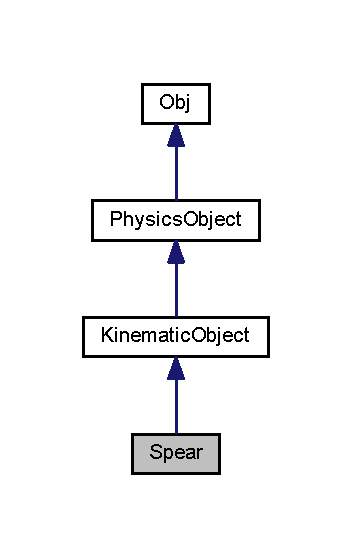
\includegraphics[width=169pt]{class_spear__inherit__graph}
\end{center}
\end{figure}


Collaboration diagram for Spear\+:
\nopagebreak
\begin{figure}[H]
\begin{center}
\leavevmode
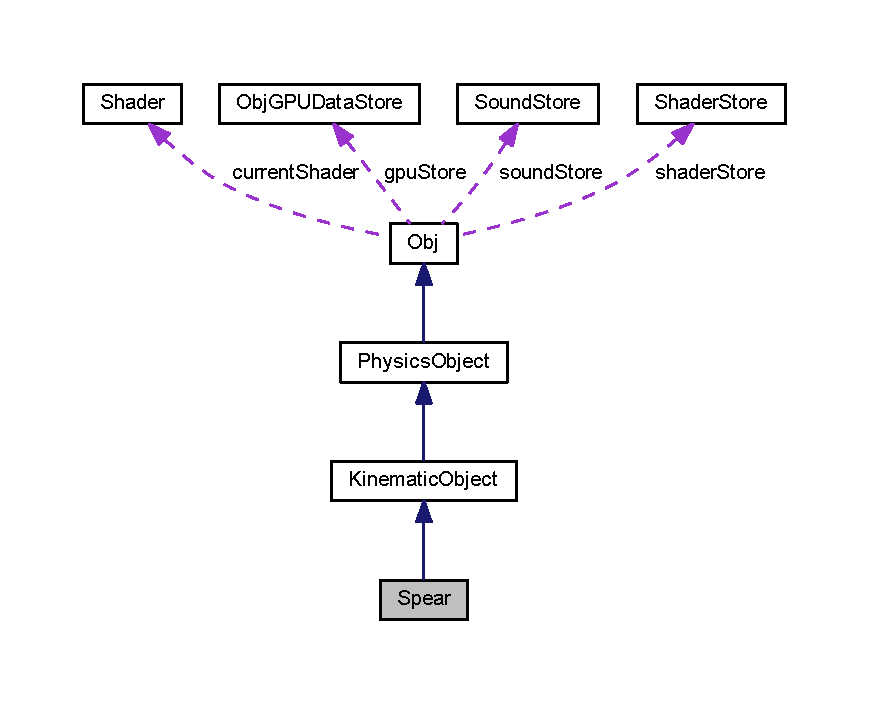
\includegraphics[width=350pt]{class_spear__coll__graph}
\end{center}
\end{figure}
\subsection*{Public Member Functions}
\begin{DoxyCompactItemize}
\item 
\hyperlink{class_spear_ab491ba668df630f8091d9da0bcbf5f56}{Spear} (float x, float y, float rotation=0.\+0f)
\begin{DoxyCompactList}\small\item\em \hyperlink{class_spear}{Spear} constructor. \end{DoxyCompactList}\end{DoxyCompactItemize}
\subsection*{Additional Inherited Members}


\subsection{Detailed Description}
The \hyperlink{class_spear}{Spear} class implements the spear hazard. 

\subsection{Constructor \& Destructor Documentation}
\index{Spear@{Spear}!Spear@{Spear}}
\index{Spear@{Spear}!Spear@{Spear}}
\subsubsection[{\texorpdfstring{Spear(float x, float y, float rotation=0.\+0f)}{Spear(float x, float y, float rotation=0.0f)}}]{\setlength{\rightskip}{0pt plus 5cm}Spear\+::\+Spear (
\begin{DoxyParamCaption}
\item[{float}]{x, }
\item[{float}]{y, }
\item[{float}]{rotation = {\ttfamily 0.0f}}
\end{DoxyParamCaption}
)}\hypertarget{class_spear_ab491ba668df630f8091d9da0bcbf5f56}{}\label{class_spear_ab491ba668df630f8091d9da0bcbf5f56}


\hyperlink{class_spear}{Spear} constructor. 


\begin{DoxyParams}{Parameters}
{\em x} & The x coordinate of the spear. \\
\hline
{\em y} & The y coordinate of the spear. \\
\hline
{\em rotation} & The rotation of the spear about the z-\/axis. \\
\hline
\end{DoxyParams}


The documentation for this class was generated from the following file\+:\begin{DoxyCompactItemize}
\item 
Spear.\+h\end{DoxyCompactItemize}

\hypertarget{class_spikes}{}\section{Spikes Class Reference}
\label{class_spikes}\index{Spikes@{Spikes}}


{\ttfamily \#include $<$Spikes.\+h$>$}



Inheritance diagram for Spikes\+:
\nopagebreak
\begin{figure}[H]
\begin{center}
\leavevmode
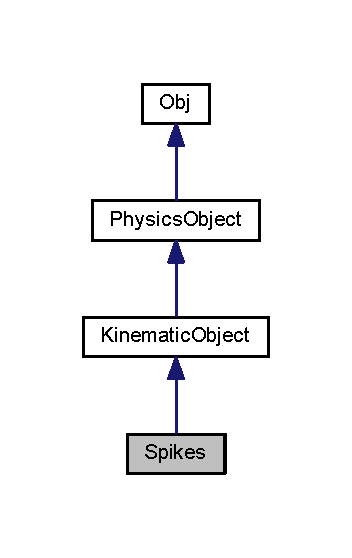
\includegraphics[width=169pt]{class_spikes__inherit__graph}
\end{center}
\end{figure}


Collaboration diagram for Spikes\+:
\nopagebreak
\begin{figure}[H]
\begin{center}
\leavevmode
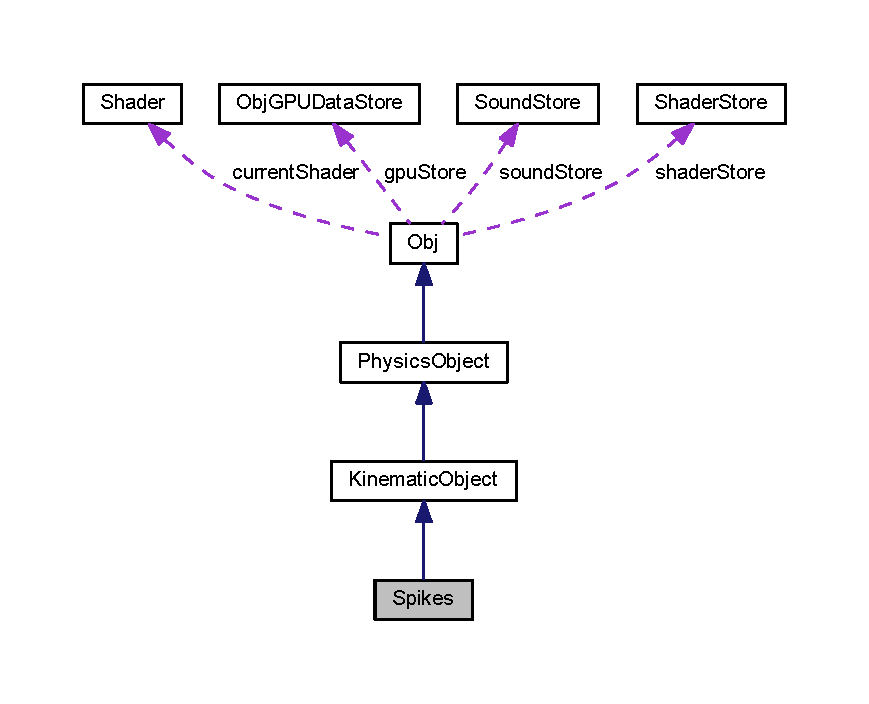
\includegraphics[width=350pt]{class_spikes__coll__graph}
\end{center}
\end{figure}
\subsection*{Public Member Functions}
\begin{DoxyCompactItemize}
\item 
\hyperlink{class_spikes_a156f940b16fe97124daca198f963cbf9}{Spikes} (float x, float y, float rotation=0.\+0f)
\begin{DoxyCompactList}\small\item\em \hyperlink{class_spikes}{Spikes} constructor. \end{DoxyCompactList}\end{DoxyCompactItemize}
\subsection*{Additional Inherited Members}


\subsection{Detailed Description}
The \hyperlink{class_spikes}{Spikes} class implements the spikes hazard. 

\subsection{Constructor \& Destructor Documentation}
\index{Spikes@{Spikes}!Spikes@{Spikes}}
\index{Spikes@{Spikes}!Spikes@{Spikes}}
\subsubsection[{\texorpdfstring{Spikes(float x, float y, float rotation=0.\+0f)}{Spikes(float x, float y, float rotation=0.0f)}}]{\setlength{\rightskip}{0pt plus 5cm}Spikes\+::\+Spikes (
\begin{DoxyParamCaption}
\item[{float}]{x, }
\item[{float}]{y, }
\item[{float}]{rotation = {\ttfamily 0.0f}}
\end{DoxyParamCaption}
)}\hypertarget{class_spikes_a156f940b16fe97124daca198f963cbf9}{}\label{class_spikes_a156f940b16fe97124daca198f963cbf9}


\hyperlink{class_spikes}{Spikes} constructor. 


\begin{DoxyParams}{Parameters}
{\em x} & The x coordinate of the spikes. \\
\hline
{\em y} & The y coordinate of the spikes. \\
\hline
{\em rotation} & The rotation of the spikes about the z-\/axis. \\
\hline
\end{DoxyParams}


The documentation for this class was generated from the following file\+:\begin{DoxyCompactItemize}
\item 
Spikes.\+h\end{DoxyCompactItemize}

\hypertarget{class_stage}{}\section{Stage Class Reference}
\label{class_stage}\index{Stage@{Stage}}


{\ttfamily \#include $<$Stage.\+h$>$}



Inheritance diagram for Stage\+:
\nopagebreak
\begin{figure}[H]
\begin{center}
\leavevmode
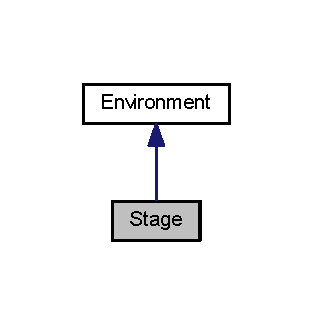
\includegraphics[width=150pt]{class_stage__inherit__graph}
\end{center}
\end{figure}


Collaboration diagram for Stage\+:
\nopagebreak
\begin{figure}[H]
\begin{center}
\leavevmode
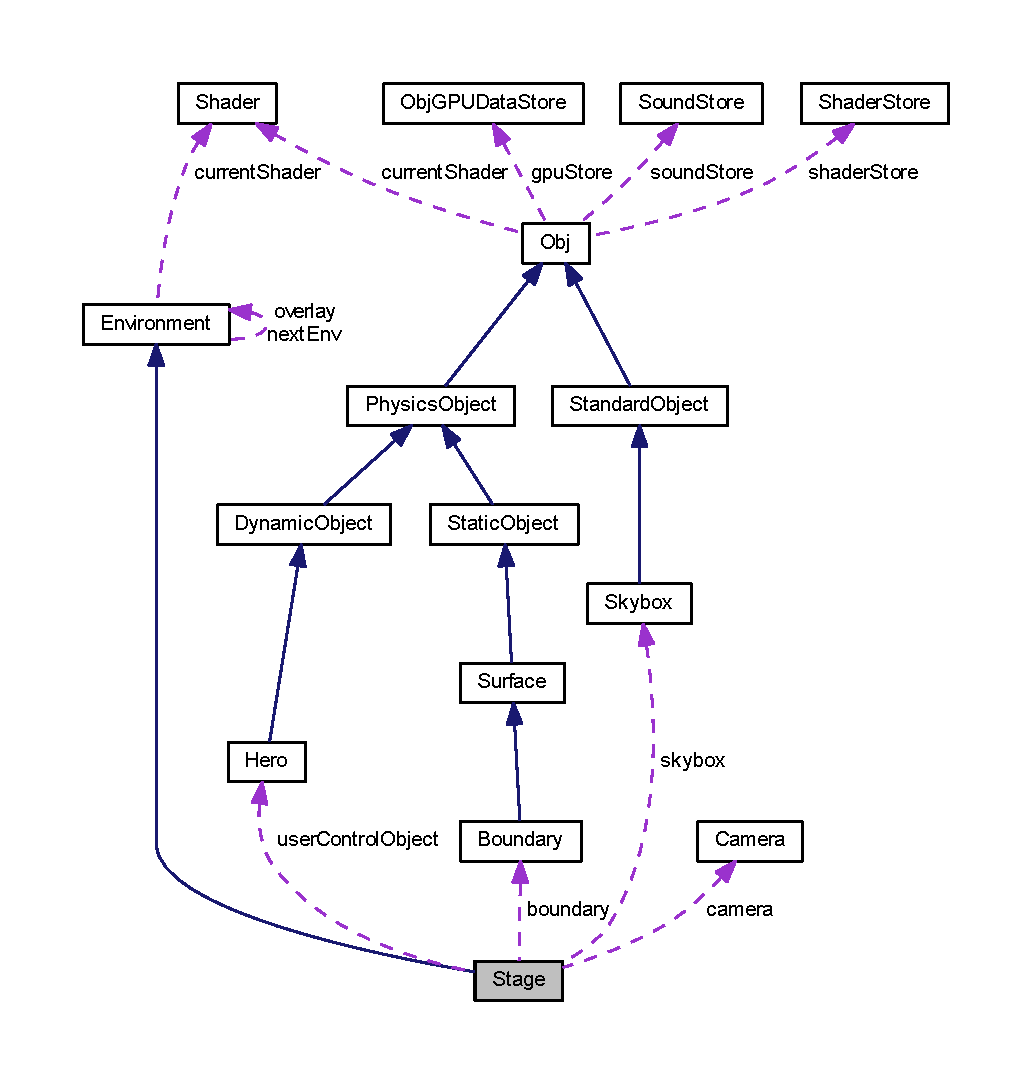
\includegraphics[width=350pt]{class_stage__coll__graph}
\end{center}
\end{figure}
\subsection*{Public Member Functions}
\begin{DoxyCompactItemize}
\item 
\hyperlink{class_stage_a2ea3892c2b58307b9b47c9ef154bf4ab}{Stage} (std\+::string \hyperlink{class_stage_a6db07a70fa2bbc7ef6e92be5d43181b9}{stage\+Name})\hypertarget{class_stage_a2ea3892c2b58307b9b47c9ef154bf4ab}{}\label{class_stage_a2ea3892c2b58307b9b47c9ef154bf4ab}

\begin{DoxyCompactList}\small\item\em \hyperlink{class_stage}{Stage} constructor. \end{DoxyCompactList}\item 
\hyperlink{class_stage_af769a51df1efaaa5fca98008fb6f0c16}{$\sim$\+Stage} ()\hypertarget{class_stage_af769a51df1efaaa5fca98008fb6f0c16}{}\label{class_stage_af769a51df1efaaa5fca98008fb6f0c16}

\begin{DoxyCompactList}\small\item\em \hyperlink{class_stage}{Stage} destructor. \end{DoxyCompactList}\item 
void \hyperlink{class_stage_a3b0abe7d74c6d38cfedeab84a7506816}{update\+Environment} (double dt)
\begin{DoxyCompactList}\small\item\em Function for updating the environment. \end{DoxyCompactList}\item 
void \hyperlink{class_stage_a550f7504d9f1eb45a1f0a24c29b58fc8}{draw\+Environment} ()\hypertarget{class_stage_a550f7504d9f1eb45a1f0a24c29b58fc8}{}\label{class_stage_a550f7504d9f1eb45a1f0a24c29b58fc8}

\begin{DoxyCompactList}\small\item\em Function for drawing the environment. \end{DoxyCompactList}\item 
void \hyperlink{class_stage_ab0ac39aba2fa162499d2599c981ca3ed}{process\+KB} (int key, int scancode, int action, int mods)
\begin{DoxyCompactList}\small\item\em Function for keyboard input processing. \end{DoxyCompactList}\item 
void \hyperlink{class_stage_a92feebde5c5fd84711ce19f0e4d07552}{process\+Continuous\+Input} ()\hypertarget{class_stage_a92feebde5c5fd84711ce19f0e4d07552}{}\label{class_stage_a92feebde5c5fd84711ce19f0e4d07552}

\begin{DoxyCompactList}\small\item\em Function for continuous input processing. \end{DoxyCompactList}\item 
bool \hyperlink{class_stage_ad3210cb8d424925079ced7a8b4bb6398}{process\+Mouse\+Position} (float xpos, float ypos)
\begin{DoxyCompactList}\small\item\em Function for mouse position change processing. \end{DoxyCompactList}\item 
void \hyperlink{class_stage_a7b45f13e5fa53354af729d022842a4de}{process\+Mouse\+Click} (int button, int action, int mods)
\begin{DoxyCompactList}\small\item\em Function for mouse input processing. \end{DoxyCompactList}\item 
bool \hyperlink{class_stage_a6f65f2412b7f72e508ac46889dcca0b6}{check\+Completion} ()
\begin{DoxyCompactList}\small\item\em Checks if stage is complete. \end{DoxyCompactList}\item 
void \hyperlink{class_stage_a51e37b7168f0af367ae6cc7dca5949b3}{update\+Screen\+Size} ()\hypertarget{class_stage_a51e37b7168f0af367ae6cc7dca5949b3}{}\label{class_stage_a51e37b7168f0af367ae6cc7dca5949b3}

\begin{DoxyCompactList}\small\item\em Updates the projection matrix when screen size is changed. \end{DoxyCompactList}\end{DoxyCompactItemize}
\subsection*{Private Member Functions}
\begin{DoxyCompactItemize}
\item 
void \hyperlink{class_stage_a737a4dd0f7e54b3a97ddd13b88a0516e}{draw\+Obj} (\hyperlink{class_physics_object}{Physics\+Object} current\+Obj, bool is\+Boundary=false)
\begin{DoxyCompactList}\small\item\em Draws an object. \end{DoxyCompactList}\end{DoxyCompactItemize}
\subsection*{Private Attributes}
\begin{DoxyCompactItemize}
\item 
cp\+Space $\ast$ \hyperlink{class_stage_a76084dcddff87933d320310c0dd3e0c9}{env\+Space}\hypertarget{class_stage_a76084dcddff87933d320310c0dd3e0c9}{}\label{class_stage_a76084dcddff87933d320310c0dd3e0c9}

\begin{DoxyCompactList}\small\item\em Pointer to the chipmunk space associated with the stage. \end{DoxyCompactList}\item 
std\+::vector$<$ \hyperlink{class_physics_object}{Physics\+Object} $\ast$ $>$ \hyperlink{class_stage_a2eff484024263e8dac366acceaf39d80}{physics\+Objects}\hypertarget{class_stage_a2eff484024263e8dac366acceaf39d80}{}\label{class_stage_a2eff484024263e8dac366acceaf39d80}

\begin{DoxyCompactList}\small\item\em List of physics objects (excluding kinematic) in stage. \end{DoxyCompactList}\item 
std\+::vector$<$ \hyperlink{class_kinematic_object}{Kinematic\+Object} $\ast$ $>$ \hyperlink{class_stage_ae19e1e3837dbfce1b5b56baea357257c}{kinematic\+Objects}\hypertarget{class_stage_ae19e1e3837dbfce1b5b56baea357257c}{}\label{class_stage_ae19e1e3837dbfce1b5b56baea357257c}

\begin{DoxyCompactList}\small\item\em List of kinematic objects in stage. \end{DoxyCompactList}\item 
std\+::vector$<$ \hyperlink{class_standard_object}{Standard\+Object} $\ast$ $>$ \hyperlink{class_stage_a24a06cb21b7049ff40def14328cd9ff7}{standard\+Objects}\hypertarget{class_stage_a24a06cb21b7049ff40def14328cd9ff7}{}\label{class_stage_a24a06cb21b7049ff40def14328cd9ff7}

\begin{DoxyCompactList}\small\item\em List of standard objects in stage. \end{DoxyCompactList}\item 
\hyperlink{class_skybox}{Skybox} $\ast$ \hyperlink{class_stage_a6f4ee2ce2aa9c87d5f97088b7e303fd6}{skybox}\hypertarget{class_stage_a6f4ee2ce2aa9c87d5f97088b7e303fd6}{}\label{class_stage_a6f4ee2ce2aa9c87d5f97088b7e303fd6}

\begin{DoxyCompactList}\small\item\em The skybox object provides the backdrop of the stage. \end{DoxyCompactList}\item 
\hyperlink{class_boundary}{Boundary} $\ast$ \hyperlink{class_stage_a7e88ab3e92a9e1b4d12fc867a22ad99f}{boundary}\hypertarget{class_stage_a7e88ab3e92a9e1b4d12fc867a22ad99f}{}\label{class_stage_a7e88ab3e92a9e1b4d12fc867a22ad99f}

\begin{DoxyCompactList}\small\item\em The boundary object provides the surface setting. \end{DoxyCompactList}\item 
float \hyperlink{class_stage_ad88ab19f6d546610c52c564d4326092d}{stage\+Time}\hypertarget{class_stage_ad88ab19f6d546610c52c564d4326092d}{}\label{class_stage_ad88ab19f6d546610c52c564d4326092d}

\begin{DoxyCompactList}\small\item\em Time elapsed since beginning the stage. \end{DoxyCompactList}\item 
\hyperlink{class_hero}{Hero} $\ast$ \hyperlink{class_stage_a756489b3e5916985247b3e411a9f8622}{user\+Control\+Object}\hypertarget{class_stage_a756489b3e5916985247b3e411a9f8622}{}\label{class_stage_a756489b3e5916985247b3e411a9f8622}

\begin{DoxyCompactList}\small\item\em Pointer to the dynamic object that is controlled by the user (normally the hero object). \end{DoxyCompactList}\item 
\hyperlink{class_camera}{Camera} \hyperlink{class_stage_a88bbb5be32cbda115a81dab24b2d4339}{camera}\hypertarget{class_stage_a88bbb5be32cbda115a81dab24b2d4339}{}\label{class_stage_a88bbb5be32cbda115a81dab24b2d4339}

\begin{DoxyCompactList}\small\item\em Used to control the view. \end{DoxyCompactList}\item 
int \hyperlink{class_stage_a3f43ef5fd16f416045a8a5f073d5edd6}{win\+Timer}\hypertarget{class_stage_a3f43ef5fd16f416045a8a5f073d5edd6}{}\label{class_stage_a3f43ef5fd16f416045a8a5f073d5edd6}

\begin{DoxyCompactList}\small\item\em Countdown timer set when stage is won; determines when exit to menu occurs. \end{DoxyCompactList}\item 
std\+::string \hyperlink{class_stage_a6db07a70fa2bbc7ef6e92be5d43181b9}{stage\+Name}\hypertarget{class_stage_a6db07a70fa2bbc7ef6e92be5d43181b9}{}\label{class_stage_a6db07a70fa2bbc7ef6e92be5d43181b9}

\begin{DoxyCompactList}\small\item\em Name of current stage file (used for reseting stage). \end{DoxyCompactList}\end{DoxyCompactItemize}
\subsection*{Additional Inherited Members}


\subsection{Detailed Description}
The \hyperlink{class_stage}{Stage} class is derived from the \hyperlink{class_environment}{Environment} class and holds and handles changes to the game state when the user is playing a stage. 

\subsection{Member Function Documentation}
\index{Stage@{Stage}!check\+Completion@{check\+Completion}}
\index{check\+Completion@{check\+Completion}!Stage@{Stage}}
\subsubsection[{\texorpdfstring{check\+Completion()}{checkCompletion()}}]{\setlength{\rightskip}{0pt plus 5cm}bool Stage\+::check\+Completion (
\begin{DoxyParamCaption}
{}
\end{DoxyParamCaption}
)}\hypertarget{class_stage_a6f65f2412b7f72e508ac46889dcca0b6}{}\label{class_stage_a6f65f2412b7f72e508ac46889dcca0b6}


Checks if stage is complete. 

\begin{DoxyReturn}{Returns}
True if stage is complete, else false. 
\end{DoxyReturn}
\index{Stage@{Stage}!draw\+Obj@{draw\+Obj}}
\index{draw\+Obj@{draw\+Obj}!Stage@{Stage}}
\subsubsection[{\texorpdfstring{draw\+Obj(\+Physics\+Object current\+Obj, bool is\+Boundary=false)}{drawObj(PhysicsObject currentObj, bool isBoundary=false)}}]{\setlength{\rightskip}{0pt plus 5cm}void Stage\+::draw\+Obj (
\begin{DoxyParamCaption}
\item[{{\bf Physics\+Object}}]{current\+Obj, }
\item[{bool}]{is\+Boundary = {\ttfamily false}}
\end{DoxyParamCaption}
)\hspace{0.3cm}{\ttfamily [private]}}\hypertarget{class_stage_a737a4dd0f7e54b3a97ddd13b88a0516e}{}\label{class_stage_a737a4dd0f7e54b3a97ddd13b88a0516e}


Draws an object. 


\begin{DoxyParams}{Parameters}
{\em current\+Obj} & Object that should be drawn. \\
\hline
{\em is\+Boundary} & Flag for boundaries (default = false); boundaries are drawn slightly differently. \\
\hline
\end{DoxyParams}
\index{Stage@{Stage}!process\+KB@{process\+KB}}
\index{process\+KB@{process\+KB}!Stage@{Stage}}
\subsubsection[{\texorpdfstring{process\+K\+B(int key, int scancode, int action, int mods)}{processKB(int key, int scancode, int action, int mods)}}]{\setlength{\rightskip}{0pt plus 5cm}void Stage\+::process\+KB (
\begin{DoxyParamCaption}
\item[{int}]{key, }
\item[{int}]{scancode, }
\item[{int}]{action, }
\item[{int}]{mods}
\end{DoxyParamCaption}
)\hspace{0.3cm}{\ttfamily [virtual]}}\hypertarget{class_stage_ab0ac39aba2fa162499d2599c981ca3ed}{}\label{class_stage_ab0ac39aba2fa162499d2599c981ca3ed}


Function for keyboard input processing. 


\begin{DoxyParams}{Parameters}
{\em key} & Key to which the action corresponds. \\
\hline
{\em scancode} & System specific key code. \\
\hline
{\em action} & The action (i.\+e. button up, down, held, etc.) \\
\hline
{\em mods} & Active modifiers (i.\+e. shift, control, etc.) \\
\hline
\end{DoxyParams}


Implements \hyperlink{class_environment_a3a105533fb7592615f6b4321aafc5545}{Environment}.

\index{Stage@{Stage}!process\+Mouse\+Click@{process\+Mouse\+Click}}
\index{process\+Mouse\+Click@{process\+Mouse\+Click}!Stage@{Stage}}
\subsubsection[{\texorpdfstring{process\+Mouse\+Click(int button, int action, int mods)}{processMouseClick(int button, int action, int mods)}}]{\setlength{\rightskip}{0pt plus 5cm}void Stage\+::process\+Mouse\+Click (
\begin{DoxyParamCaption}
\item[{int}]{button, }
\item[{int}]{action, }
\item[{int}]{mods}
\end{DoxyParamCaption}
)\hspace{0.3cm}{\ttfamily [virtual]}}\hypertarget{class_stage_a7b45f13e5fa53354af729d022842a4de}{}\label{class_stage_a7b45f13e5fa53354af729d022842a4de}


Function for mouse input processing. 


\begin{DoxyParams}{Parameters}
{\em button} & Mouse button to which the action corresponds. \\
\hline
{\em action} & The action (i.\+e. button up, down, held, etc.) \\
\hline
{\em mods} & Active modifiers (i.\+e. shift, control, etc.) \\
\hline
\end{DoxyParams}


Implements \hyperlink{class_environment_a19cf4bbbe86528759e0ad79e19025732}{Environment}.

\index{Stage@{Stage}!process\+Mouse\+Position@{process\+Mouse\+Position}}
\index{process\+Mouse\+Position@{process\+Mouse\+Position}!Stage@{Stage}}
\subsubsection[{\texorpdfstring{process\+Mouse\+Position(float xpos, float ypos)}{processMousePosition(float xpos, float ypos)}}]{\setlength{\rightskip}{0pt plus 5cm}bool Stage\+::process\+Mouse\+Position (
\begin{DoxyParamCaption}
\item[{float}]{xpos, }
\item[{float}]{ypos}
\end{DoxyParamCaption}
)\hspace{0.3cm}{\ttfamily [virtual]}}\hypertarget{class_stage_ad3210cb8d424925079ced7a8b4bb6398}{}\label{class_stage_ad3210cb8d424925079ced7a8b4bb6398}


Function for mouse position change processing. 


\begin{DoxyParams}{Parameters}
{\em xpos} & Mouse cursor x-\/position \\
\hline
{\em ypos} & Mouse cursor y-\/position \\
\hline
\end{DoxyParams}


Implements \hyperlink{class_environment_a92819bf5a6aa5877c0f89fd65a4d7554}{Environment}.

\index{Stage@{Stage}!update\+Environment@{update\+Environment}}
\index{update\+Environment@{update\+Environment}!Stage@{Stage}}
\subsubsection[{\texorpdfstring{update\+Environment(double dt)}{updateEnvironment(double dt)}}]{\setlength{\rightskip}{0pt plus 5cm}void Stage\+::update\+Environment (
\begin{DoxyParamCaption}
\item[{double}]{dt}
\end{DoxyParamCaption}
)\hspace{0.3cm}{\ttfamily [virtual]}}\hypertarget{class_stage_a3b0abe7d74c6d38cfedeab84a7506816}{}\label{class_stage_a3b0abe7d74c6d38cfedeab84a7506816}


Function for updating the environment. 


\begin{DoxyParams}{Parameters}
{\em dt} & Time step to be used for the update (time since last update) in milliseconds. \\
\hline
\end{DoxyParams}


Implements \hyperlink{class_environment_afbc95329581e994ed49a678c814657ea}{Environment}.



The documentation for this class was generated from the following file\+:\begin{DoxyCompactItemize}
\item 
Stage.\+h\end{DoxyCompactItemize}

\hypertarget{class_stage_loader}{}\section{Stage\+Loader Class Reference}
\label{class_stage_loader}\index{Stage\+Loader@{Stage\+Loader}}


{\ttfamily \#include $<$Stage\+Loader.\+h$>$}

\subsection*{Public Member Functions}
\begin{DoxyCompactItemize}
\item 
\hyperlink{class_stage_loader_ac3db92090726b0394a18345e5a781a9d}{Stage\+Loader} (std\+::string \hyperlink{class_stage_loader_a3574f9ea01596806f37b196849bbefae}{file\+Name}, std\+::vector$<$ \hyperlink{class_physics_object}{Physics\+Object} $\ast$ $>$ \&physics\+Objects, std\+::vector$<$ \hyperlink{class_kinematic_object}{Kinematic\+Object} $\ast$ $>$ \&kinematic\+Objects, std\+::vector$<$ \hyperlink{class_standard_object}{Standard\+Object} $\ast$ $>$ \&standard\+Objects, \hyperlink{class_skybox}{Skybox} $\ast$\&skybox, \hyperlink{class_boundary}{Boundary} $\ast$\&boundary, \hyperlink{class_hero}{Hero} $\ast$\&user\+Control\+Object)
\begin{DoxyCompactList}\small\item\em \hyperlink{class_stage_loader}{Stage\+Loader} constructor. \end{DoxyCompactList}\end{DoxyCompactItemize}
\subsection*{Private Member Functions}
\begin{DoxyCompactItemize}
\item 
std\+::string \hyperlink{class_stage_loader_a4a9e517ca2cc71f73819caac034fc5a6}{strip\+Whitespace} (std\+::string str)
\begin{DoxyCompactList}\small\item\em Strips all whitespace from string. \end{DoxyCompactList}\item 
std\+::string \hyperlink{class_stage_loader_ad69aac2054f04e4ea393ae0b992416c5}{check\+Field} (std\+::string field)
\begin{DoxyCompactList}\small\item\em Checks if stage\+Info contains a key; if not reports error. \end{DoxyCompactList}\item 
void \hyperlink{class_stage_loader_a686383910433f0d5a8109e01b1ede249}{report\+Error} ()\hypertarget{class_stage_loader_a686383910433f0d5a8109e01b1ede249}{}\label{class_stage_loader_a686383910433f0d5a8109e01b1ede249}

\begin{DoxyCompactList}\small\item\em Reports error at current line. \end{DoxyCompactList}\item 
void \hyperlink{class_stage_loader_a691e32f2cea41a78d6a6e99611acb0a6}{get\+Next\+Line} ()\hypertarget{class_stage_loader_a691e32f2cea41a78d6a6e99611acb0a6}{}\label{class_stage_loader_a691e32f2cea41a78d6a6e99611acb0a6}

\begin{DoxyCompactList}\small\item\em Retrieves next line. \end{DoxyCompactList}\end{DoxyCompactItemize}
\subsection*{Private Attributes}
\begin{DoxyCompactItemize}
\item 
std\+::string \hyperlink{class_stage_loader_a3574f9ea01596806f37b196849bbefae}{file\+Name}\hypertarget{class_stage_loader_a3574f9ea01596806f37b196849bbefae}{}\label{class_stage_loader_a3574f9ea01596806f37b196849bbefae}

\begin{DoxyCompactList}\small\item\em \hyperlink{class_stage}{Stage} file path. \end{DoxyCompactList}\item 
int \hyperlink{class_stage_loader_a69303db8d3e7d91e0de14b6f7c2c08ab}{line\+No}\hypertarget{class_stage_loader_a69303db8d3e7d91e0de14b6f7c2c08ab}{}\label{class_stage_loader_a69303db8d3e7d91e0de14b6f7c2c08ab}

\begin{DoxyCompactList}\small\item\em Current line number. \end{DoxyCompactList}\item 
std\+::string \hyperlink{class_stage_loader_a8413ef9f88df043d287d92afe55f9e7a}{cur\+Line}\hypertarget{class_stage_loader_a8413ef9f88df043d287d92afe55f9e7a}{}\label{class_stage_loader_a8413ef9f88df043d287d92afe55f9e7a}

\begin{DoxyCompactList}\small\item\em Current line being parsed. \end{DoxyCompactList}\item 
std\+::string \hyperlink{class_stage_loader_a9387427e7e4ca5a9210bfac081dc048b}{line}\hypertarget{class_stage_loader_a9387427e7e4ca5a9210bfac081dc048b}{}\label{class_stage_loader_a9387427e7e4ca5a9210bfac081dc048b}

\begin{DoxyCompactList}\small\item\em Current line being parsed, stripped of whitespace. \end{DoxyCompactList}\item 
std\+::ifstream \hyperlink{class_stage_loader_a9d71f768884e3dd10f9c773a41af83e0}{in\+File}\hypertarget{class_stage_loader_a9d71f768884e3dd10f9c773a41af83e0}{}\label{class_stage_loader_a9d71f768884e3dd10f9c773a41af83e0}

\begin{DoxyCompactList}\small\item\em File stream of the input file. \end{DoxyCompactList}\item 
std\+::map$<$ std\+::string, std\+::string $>$ \hyperlink{class_stage_loader_a53604a9fc34a15e90a13abbc9813297a}{stage\+Info}\hypertarget{class_stage_loader_a53604a9fc34a15e90a13abbc9813297a}{}\label{class_stage_loader_a53604a9fc34a15e90a13abbc9813297a}

\begin{DoxyCompactList}\small\item\em Map that stores stage information. \end{DoxyCompactList}\end{DoxyCompactItemize}


\subsection{Detailed Description}
The \hyperlink{class_stage_loader}{Stage\+Loader} class parses stage files to create levels at runtime. 

\subsection{Constructor \& Destructor Documentation}
\index{Stage\+Loader@{Stage\+Loader}!Stage\+Loader@{Stage\+Loader}}
\index{Stage\+Loader@{Stage\+Loader}!Stage\+Loader@{Stage\+Loader}}
\subsubsection[{\texorpdfstring{Stage\+Loader(std\+::string file\+Name, std\+::vector$<$ Physics\+Object $\ast$ $>$ \&physics\+Objects, std\+::vector$<$ Kinematic\+Object $\ast$ $>$ \&kinematic\+Objects, std\+::vector$<$ Standard\+Object $\ast$ $>$ \&standard\+Objects, Skybox $\ast$\&skybox, Boundary $\ast$\&boundary, Hero $\ast$\&user\+Control\+Object)}{StageLoader(std::string fileName, std::vector< PhysicsObject * > &physicsObjects, std::vector< KinematicObject * > &kinematicObjects, std::vector< StandardObject * > &standardObjects, Skybox *&skybox, Boundary *&boundary, Hero *&userControlObject)}}]{\setlength{\rightskip}{0pt plus 5cm}Stage\+Loader\+::\+Stage\+Loader (
\begin{DoxyParamCaption}
\item[{std\+::string}]{file\+Name, }
\item[{std\+::vector$<$ {\bf Physics\+Object} $\ast$ $>$ \&}]{physics\+Objects, }
\item[{std\+::vector$<$ {\bf Kinematic\+Object} $\ast$ $>$ \&}]{kinematic\+Objects, }
\item[{std\+::vector$<$ {\bf Standard\+Object} $\ast$ $>$ \&}]{standard\+Objects, }
\item[{{\bf Skybox} $\ast$\&}]{skybox, }
\item[{{\bf Boundary} $\ast$\&}]{boundary, }
\item[{{\bf Hero} $\ast$\&}]{user\+Control\+Object}
\end{DoxyParamCaption}
)}\hypertarget{class_stage_loader_ac3db92090726b0394a18345e5a781a9d}{}\label{class_stage_loader_ac3db92090726b0394a18345e5a781a9d}


\hyperlink{class_stage_loader}{Stage\+Loader} constructor. 


\begin{DoxyParams}{Parameters}
{\em file\+Name} & The path to the stage file. \\
\hline
{\em physics\+Objects} & Reference to vector to be filled with physics objects. \\
\hline
{\em kinematic\+Objects} & Reference to vector to be filled with kinematic objects. \\
\hline
{\em standard\+Objects} & Reference to vector to be filled with standard objects. \\
\hline
{\em skybox} & Reference to \hyperlink{class_skybox}{Skybox} to be populated by skybox object. \\
\hline
{\em boundary} & Reference to \hyperlink{class_boundary}{Boundary} to be populated by boundary object. \\
\hline
{\em user\+Control\+Object} & Reference to \hyperlink{class_hero}{Hero} to be populated with the hero object. \\
\hline
\end{DoxyParams}


\subsection{Member Function Documentation}
\index{Stage\+Loader@{Stage\+Loader}!check\+Field@{check\+Field}}
\index{check\+Field@{check\+Field}!Stage\+Loader@{Stage\+Loader}}
\subsubsection[{\texorpdfstring{check\+Field(std\+::string field)}{checkField(std::string field)}}]{\setlength{\rightskip}{0pt plus 5cm}std\+::string Stage\+Loader\+::check\+Field (
\begin{DoxyParamCaption}
\item[{std\+::string}]{field}
\end{DoxyParamCaption}
)\hspace{0.3cm}{\ttfamily [private]}}\hypertarget{class_stage_loader_ad69aac2054f04e4ea393ae0b992416c5}{}\label{class_stage_loader_ad69aac2054f04e4ea393ae0b992416c5}


Checks if stage\+Info contains a key; if not reports error. 


\begin{DoxyParams}{Parameters}
{\em field} & The field to be checked. \\
\hline
\end{DoxyParams}
\begin{DoxyReturn}{Returns}
The value paired with the key. 
\end{DoxyReturn}
\index{Stage\+Loader@{Stage\+Loader}!strip\+Whitespace@{strip\+Whitespace}}
\index{strip\+Whitespace@{strip\+Whitespace}!Stage\+Loader@{Stage\+Loader}}
\subsubsection[{\texorpdfstring{strip\+Whitespace(std\+::string str)}{stripWhitespace(std::string str)}}]{\setlength{\rightskip}{0pt plus 5cm}std\+::string Stage\+Loader\+::strip\+Whitespace (
\begin{DoxyParamCaption}
\item[{std\+::string}]{str}
\end{DoxyParamCaption}
)\hspace{0.3cm}{\ttfamily [private]}}\hypertarget{class_stage_loader_a4a9e517ca2cc71f73819caac034fc5a6}{}\label{class_stage_loader_a4a9e517ca2cc71f73819caac034fc5a6}


Strips all whitespace from string. 


\begin{DoxyParams}{Parameters}
{\em str} & The string to be stripped. \\
\hline
\end{DoxyParams}
\begin{DoxyReturn}{Returns}
Whitespace stripped string. 
\end{DoxyReturn}


The documentation for this class was generated from the following file\+:\begin{DoxyCompactItemize}
\item 
Stage\+Loader.\+h\end{DoxyCompactItemize}

\hypertarget{class_standard_object}{}\section{Standard\+Object Class Reference}
\label{class_standard_object}\index{Standard\+Object@{Standard\+Object}}


{\ttfamily \#include $<$Standard\+Object.\+h$>$}



Inheritance diagram for Standard\+Object\+:
\nopagebreak
\begin{figure}[H]
\begin{center}
\leavevmode
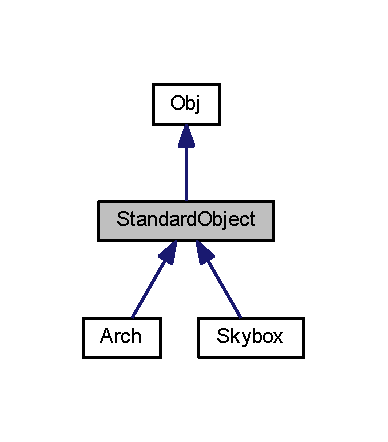
\includegraphics[width=186pt]{class_standard_object__inherit__graph}
\end{center}
\end{figure}


Collaboration diagram for Standard\+Object\+:
\nopagebreak
\begin{figure}[H]
\begin{center}
\leavevmode
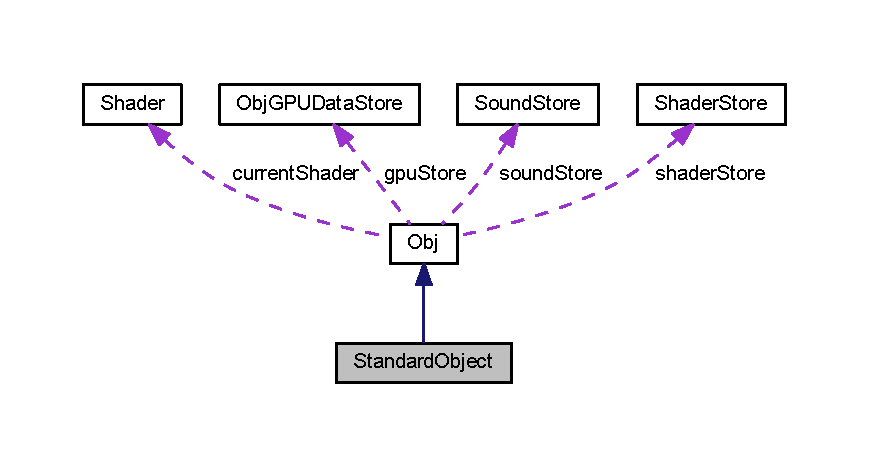
\includegraphics[width=350pt]{class_standard_object__coll__graph}
\end{center}
\end{figure}
\subsection*{Public Member Functions}
\begin{DoxyCompactItemize}
\item 
void \hyperlink{class_standard_object_a6f7910abadbf3b485b96b11c32f8a1be}{render} ()\hypertarget{class_standard_object_a6f7910abadbf3b485b96b11c32f8a1be}{}\label{class_standard_object_a6f7910abadbf3b485b96b11c32f8a1be}

\begin{DoxyCompactList}\small\item\em Renders the object. \end{DoxyCompactList}\end{DoxyCompactItemize}
\subsection*{Public Attributes}
\begin{DoxyCompactItemize}
\item 
glm\+::vec3 \hyperlink{class_standard_object_a8b6ed66159dfded1624720417d20a6c4}{position}\hypertarget{class_standard_object_a8b6ed66159dfded1624720417d20a6c4}{}\label{class_standard_object_a8b6ed66159dfded1624720417d20a6c4}

\begin{DoxyCompactList}\small\item\em Object position. \end{DoxyCompactList}\item 
float \hyperlink{class_standard_object_a7cafbb9e057f7629dbbb835612af7ae2}{angle}\hypertarget{class_standard_object_a7cafbb9e057f7629dbbb835612af7ae2}{}\label{class_standard_object_a7cafbb9e057f7629dbbb835612af7ae2}

\begin{DoxyCompactList}\small\item\em Object rotation about z-\/axis. \end{DoxyCompactList}\end{DoxyCompactItemize}
\subsection*{Additional Inherited Members}


\subsection{Detailed Description}
The \hyperlink{class_standard_object}{Standard\+Object} class is derived from the \hyperlink{class_obj}{Obj} class and is the parent to all objects that do not take part in physics/collision calculations. 

The documentation for this class was generated from the following file\+:\begin{DoxyCompactItemize}
\item 
Standard\+Object.\+h\end{DoxyCompactItemize}

\hypertarget{class_static_object}{}\section{Static\+Object Class Reference}
\label{class_static_object}\index{Static\+Object@{Static\+Object}}


{\ttfamily \#include $<$Obj.\+h$>$}

Inheritance diagram for Static\+Object\+:\begin{figure}[H]
\begin{center}
\leavevmode
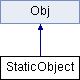
\includegraphics[height=2.000000cm]{class_static_object}
\end{center}
\end{figure}
\subsection*{Public Member Functions}
\begin{DoxyCompactItemize}
\item 
\hyperlink{class_static_object_a7d12320f994eb290f969717744bd328b}{Static\+Object} (cp\+Space $\ast$space, cp\+Vect p1, cp\+Vect p2, \hyperlink{class_obj_g_p_u_data}{Obj\+G\+P\+U\+Data} $\ast$\hyperlink{class_obj_a33a9a5371319a410f7d2d395a7ef2423}{gpu\+Data})
\begin{DoxyCompactList}\small\item\em \hyperlink{class_static_object}{Static\+Object} constructor. \end{DoxyCompactList}\end{DoxyCompactItemize}
\subsection*{Additional Inherited Members}


\subsection{Detailed Description}
The \hyperlink{class_static_object}{Static\+Object} class is derived from the \hyperlink{class_obj}{Obj} class. Physics calculations are generally ignored for static objects. Used primarily for boundaries and stationary platforms. 

\subsection{Constructor \& Destructor Documentation}
\index{Static\+Object@{Static\+Object}!Static\+Object@{Static\+Object}}
\index{Static\+Object@{Static\+Object}!Static\+Object@{Static\+Object}}
\subsubsection[{\texorpdfstring{Static\+Object(cp\+Space $\ast$space, cp\+Vect p1, cp\+Vect p2, Obj\+G\+P\+U\+Data $\ast$gpu\+Data)}{StaticObject(cpSpace *space, cpVect p1, cpVect p2, ObjGPUData *gpuData)}}]{\setlength{\rightskip}{0pt plus 5cm}Static\+Object\+::\+Static\+Object (
\begin{DoxyParamCaption}
\item[{cp\+Space $\ast$}]{space, }
\item[{cp\+Vect}]{p1, }
\item[{cp\+Vect}]{p2, }
\item[{{\bf Obj\+G\+P\+U\+Data} $\ast$}]{gpu\+Data}
\end{DoxyParamCaption}
)}\hypertarget{class_static_object_a7d12320f994eb290f969717744bd328b}{}\label{class_static_object_a7d12320f994eb290f969717744bd328b}


\hyperlink{class_static_object}{Static\+Object} constructor. 


\begin{DoxyParams}{Parameters}
{\em space} & Chipmunk 2D space to attach object to \\
\hline
{\em p1} & Bottom left coordinate of bounding box \\
\hline
{\em p2} & Upper right coordinate of bounding box \\
\hline
{\em gpu\+Data} & Pointer to the gpu data associated with the object \\
\hline
\end{DoxyParams}

\hypertarget{class_surface}{}\section{Surface Class Reference}
\label{class_surface}\index{Surface@{Surface}}


{\ttfamily \#include $<$Surface.\+h$>$}



Inheritance diagram for Surface\+:
\nopagebreak
\begin{figure}[H]
\begin{center}
\leavevmode
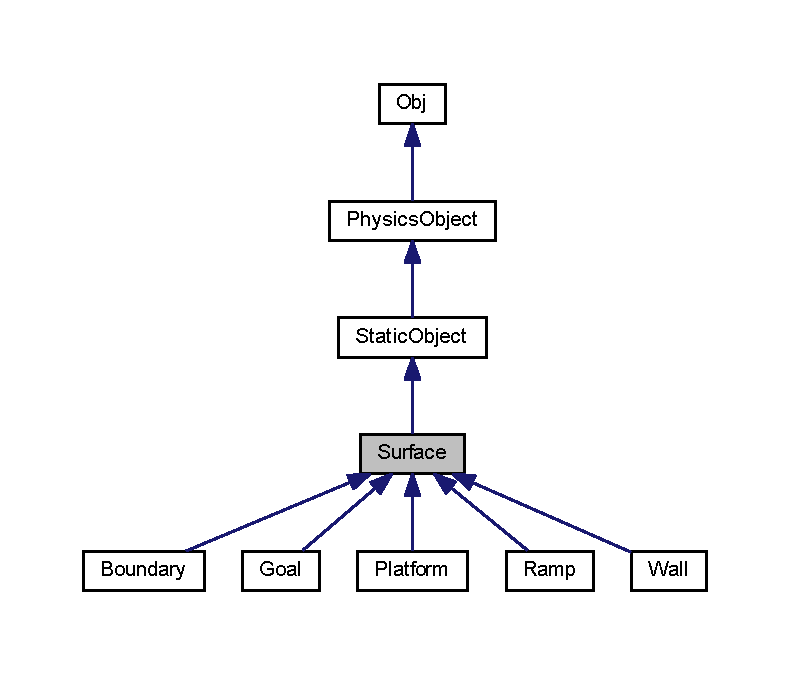
\includegraphics[width=350pt]{class_surface__inherit__graph}
\end{center}
\end{figure}


Collaboration diagram for Surface\+:
\nopagebreak
\begin{figure}[H]
\begin{center}
\leavevmode
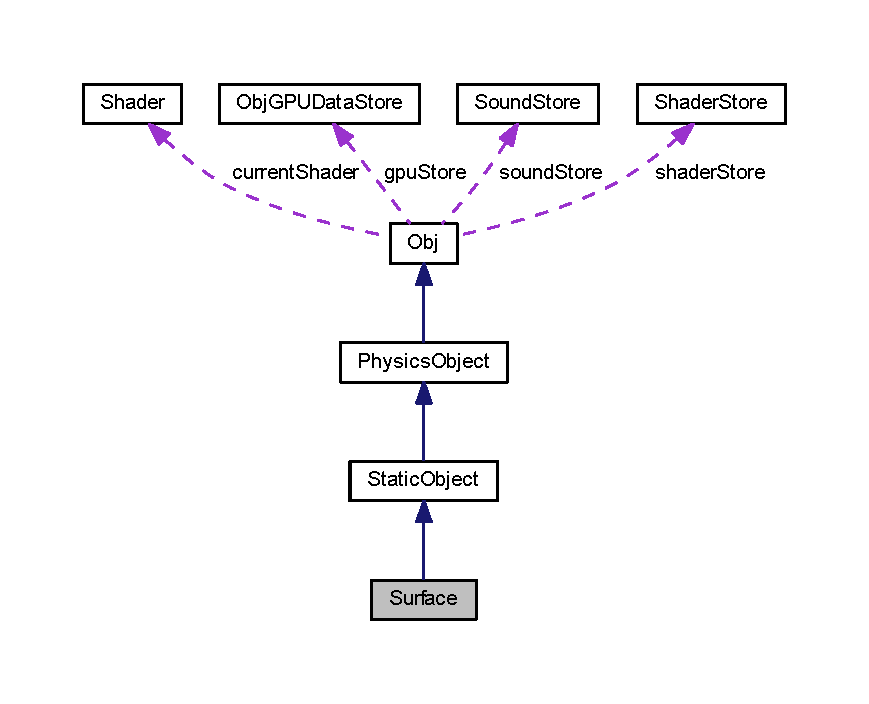
\includegraphics[width=350pt]{class_surface__coll__graph}
\end{center}
\end{figure}
\subsection*{Public Member Functions}
\begin{DoxyCompactItemize}
\item 
\hyperlink{class_surface_a4c6cf268842feb8f6fc5dffbc09a1f8f}{Surface} (cp\+Vect p1, cp\+Vect p2, bool is\+Ramp, float thickness=50.\+0f)
\begin{DoxyCompactList}\small\item\em \hyperlink{class_surface}{Surface} constructor. \end{DoxyCompactList}\end{DoxyCompactItemize}
\subsection*{Additional Inherited Members}


\subsection{Detailed Description}
The \hyperlink{class_surface}{Surface} class is derived from the \hyperlink{class_static_object}{Static\+Object} class. Used primarily for stationary platforms. 

\subsection{Constructor \& Destructor Documentation}
\index{Surface@{Surface}!Surface@{Surface}}
\index{Surface@{Surface}!Surface@{Surface}}
\subsubsection[{\texorpdfstring{Surface(cp\+Vect p1, cp\+Vect p2, bool is\+Ramp, float thickness=50.\+0f)}{Surface(cpVect p1, cpVect p2, bool isRamp, float thickness=50.0f)}}]{\setlength{\rightskip}{0pt plus 5cm}Surface\+::\+Surface (
\begin{DoxyParamCaption}
\item[{cp\+Vect}]{p1, }
\item[{cp\+Vect}]{p2, }
\item[{bool}]{is\+Ramp, }
\item[{float}]{thickness = {\ttfamily 50.0f}}
\end{DoxyParamCaption}
)}\hypertarget{class_surface_a4c6cf268842feb8f6fc5dffbc09a1f8f}{}\label{class_surface_a4c6cf268842feb8f6fc5dffbc09a1f8f}


\hyperlink{class_surface}{Surface} constructor. 


\begin{DoxyParams}{Parameters}
{\em p1} & Bottom left coordinate of bounding box \\
\hline
{\em p2} & Upper right coordinate of bounding box \\
\hline
{\em is\+Ramp} & Flag specifies if surface is a ramp \\
\hline
{\em thickness} & Thickness of the surface \\
\hline
\end{DoxyParams}


The documentation for this class was generated from the following file\+:\begin{DoxyCompactItemize}
\item 
Surface.\+h\end{DoxyCompactItemize}

\hypertarget{class_wall}{}\section{Wall Class Reference}
\label{class_wall}\index{Wall@{Wall}}


{\ttfamily \#include $<$Wall.\+h$>$}



Inheritance diagram for Wall\+:
\nopagebreak
\begin{figure}[H]
\begin{center}
\leavevmode
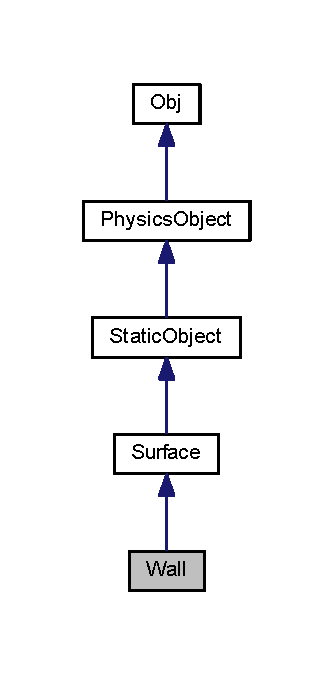
\includegraphics[width=160pt]{class_wall__inherit__graph}
\end{center}
\end{figure}


Collaboration diagram for Wall\+:
\nopagebreak
\begin{figure}[H]
\begin{center}
\leavevmode
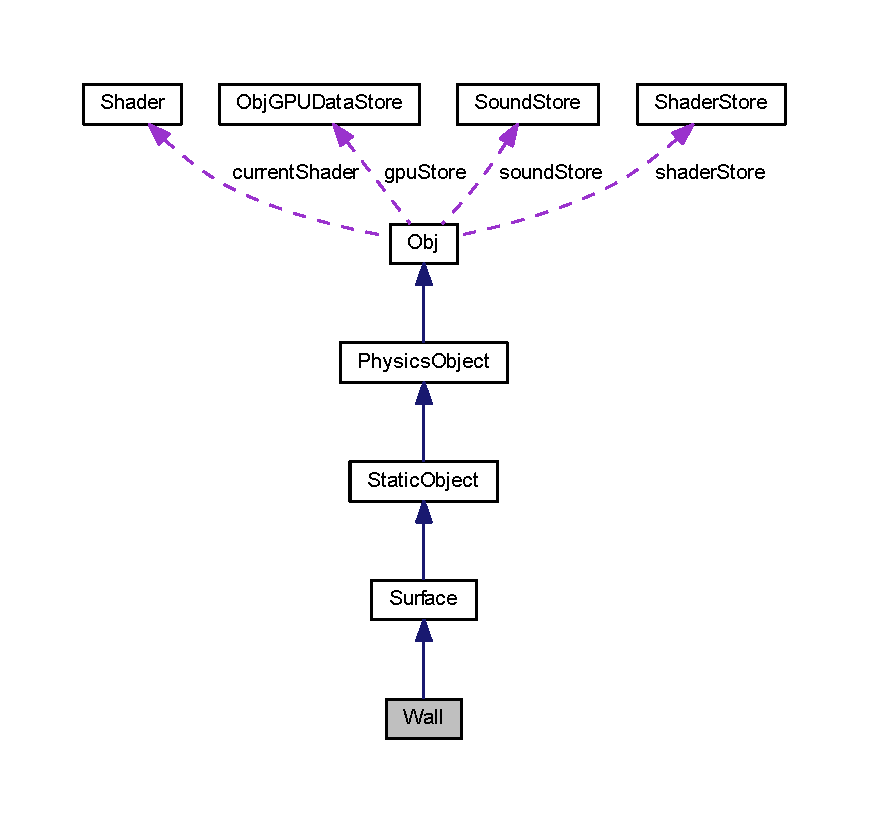
\includegraphics[width=350pt]{class_wall__coll__graph}
\end{center}
\end{figure}
\subsection*{Public Member Functions}
\begin{DoxyCompactItemize}
\item 
\hyperlink{class_wall_ae7c837d187a9728bdc27ec2edcc42476}{Wall} (float y1, float y2, float xmid, float thickness=50.\+0f)
\begin{DoxyCompactList}\small\item\em \hyperlink{class_wall}{Wall} constructor. \end{DoxyCompactList}\end{DoxyCompactItemize}
\subsection*{Additional Inherited Members}


\subsection{Detailed Description}
The \hyperlink{class_wall}{Wall} class implements wall objects. 

\subsection{Constructor \& Destructor Documentation}
\index{Wall@{Wall}!Wall@{Wall}}
\index{Wall@{Wall}!Wall@{Wall}}
\subsubsection[{\texorpdfstring{Wall(float y1, float y2, float xmid, float thickness=50.\+0f)}{Wall(float y1, float y2, float xmid, float thickness=50.0f)}}]{\setlength{\rightskip}{0pt plus 5cm}Wall\+::\+Wall (
\begin{DoxyParamCaption}
\item[{float}]{y1, }
\item[{float}]{y2, }
\item[{float}]{xmid, }
\item[{float}]{thickness = {\ttfamily 50.0f}}
\end{DoxyParamCaption}
)}\hypertarget{class_wall_ae7c837d187a9728bdc27ec2edcc42476}{}\label{class_wall_ae7c837d187a9728bdc27ec2edcc42476}


\hyperlink{class_wall}{Wall} constructor. 


\begin{DoxyParams}{Parameters}
{\em y1} & The bottom y-\/coordinate of the wall. \\
\hline
{\em y2} & The top y-\/coordinate of the wall. \\
\hline
{\em xmid} & The x-\/coordinate of the wall. \\
\hline
{\em thickness} & The horizontal thickness of the wall (default = 50.\+0). \\
\hline
\end{DoxyParams}


The documentation for this class was generated from the following file\+:\begin{DoxyCompactItemize}
\item 
Wall.\+h\end{DoxyCompactItemize}

%--- End generated contents ---

% Index
\backmatter
\newpage
\phantomsection
\clearemptydoublepage
\addcontentsline{toc}{chapter}{Index}
\printindex

\end{document}
